\documentclass{article}

\usepackage[paper=a4paper,margin=0.9in]{geometry}

\usepackage{mathtools}
\usepackage[italic=true]{derivative}
\usepackage{graphicx}
\usepackage{enumitem} % enumeration label options
\usepackage{amsfonts} % \mathbb, ...
\usepackage{amssymb} % \subsetneq, \nmid, ...
\usepackage{stmaryrd} % \mapsfrom
\usepackage{yhmath} % \widehat
\usepackage{tikz-cd}
\usepackage{amsthm}
\usepackage{dynkin-diagrams}
\usepackage{cancel}
\usepackage{parskip}
\usepackage{hyperref}

\newtheorem*{conjecture}{Conjecture}
\newtheorem*{theorem}{Theorem}
\newtheorem*{lemma}{Lemma}
\newtheorem*{proposition}{Proposition}
\newtheorem*{corollary}{Corollary}
\newtheorem*{claim}{Claim}

\theoremstyle{definition}
\newtheorem*{definition}{Definition}
\newtheorem*{fact}{Fact}
\newtheorem*{example}{Example}
\newtheorem*{nonexample}{Non-Example}
\newtheorem*{remark}{Remark}
\newtheorem*{exercise}{Exercise}

\DeclareMathOperator{\Spec}{Spec}
\DeclareMathOperator{\Proj}{Proj}
\DeclareMathOperator{\Hom}{Hom}
\DeclareMathOperator{\Hol}{Hol}
\DeclareMathOperator{\End}{End}
\DeclareMathOperator{\Aut}{Aut}
\DeclareMathOperator{\Gr}{Gr}
\DeclareMathOperator{\Sp}{Sp}
\DeclareMathOperator{\SO}{SO}
\DeclareMathOperator{\SU}{SU}
\DeclareMathOperator{\SL}{SL}
\DeclareMathOperator{\PSL}{PSL}
\DeclareMathOperator{\GL}{GL}
\DeclareMathOperator{\so}{\mathfrak{so}}
\DeclareMathOperator{\im}{im}
\DeclareMathOperator{\tr}{tr}
\DeclareMathOperator{\lk}{lk}
\DeclareMathOperator{\gr}{gr}
\DeclareMathOperator{\rad}{rad}
\DeclareMathOperator{\sgn}{sgn}
\DeclareMathOperator{\rank}{rank}
\DeclareMathOperator{\Sym}{Sym}
\DeclareMathOperator{\Vect}{Vect}
\DeclareMathOperator{\Bl}{Bl}
\DeclareMathOperator{\Diff}{Diff}
\DeclareMathOperator{\Crit}{Crit}
\DeclareMathOperator{\Hess}{Hess}
\DeclareMathOperator{\ind}{ind}
\DeclareMathOperator{\Stab}{Stab}

\newcommand{\conj}[1]{\overline{#1}}
\newcommand{\closure}[1]{\overline{#1}}

\newcommand{\id}{\mathrm{id}}
\newcommand{\ev}{\mathrm{ev}}
\newcommand{\inc}{\mathrm{inc}}
\newcommand{\cl}{\mathrm{cl}}
\newcommand{\an}{\mathrm{an}}
\newcommand{\sing}{\mathrm{sing}}
\newcommand{\dR}{\mathrm{dR}}
\newcommand{\CH}{\mathrm{CH}}
\newcommand{\Hdg}{\mathrm{Hdg}}
\newcommand{\FS}{\mathrm{FS}}
\newcommand{\PD}{\mathrm{PD}}
\newcommand{\homeo}{\mathrm{homeo}}
\newcommand{\diffeo}{\mathrm{diffeo}}

\newcommand{\calY}{\mathcal{Y}}
\newcommand{\calH}{\mathcal{H}}
\newcommand{\calJ}{\mathcal{J}}
\newcommand{\g}{\mathfrak{g}}
\newcommand{\calN}{\mathcal{N}}
\renewcommand{\L}{\mathcal{L}}
\renewcommand{\O}{\mathcal{O}}
\newcommand{\E}{\mathcal{E}}
\newcommand{\U}{\mathcal{U}}
\renewcommand{\u}{\mathfrak{u}}
\newcommand{\m}{\mathfrak{m}}
\newcommand{\RP}{\mathbb{RP}}
\newcommand{\CP}{\mathbb{CP}}
\newcommand{\HP}{\mathbb{HP}}
\renewcommand{\S}{\mathbb{S}}
\newcommand{\T}{\mathbb{T}}
\newcommand{\F}{\mathbb{F}}
\renewcommand{\H}{\mathbb{H}}
\newcommand{\bbO}{\mathbb{O}}
\renewcommand{\P}{\mathbb{P}}
\newcommand{\A}{\mathbb{A}}
\newcommand{\N}{\mathbb{N}}
\newcommand{\Z}{\mathbb{Z}}
\newcommand{\Q}{\mathbb{Q}}
\newcommand{\R}{\mathbb{R}}
\newcommand{\C}{\mathbb{C}}

\title{LSGNT 2023-2024: Topics in Geometry}
\author{}
\date{}

\begin{document}

\maketitle

\tableofcontents

\newpage

\section{Spec and Proj - Ed Segal}

\subsection*{Exercises}

\begin{enumerate}
    \item A variety $V$ is called \emph{irreducible} if it can't be decomposed
        as $V=V_1\cup V_2$ in a non-trivial way. Show that this is equivalent to
        (a) any two Zariski open subsets in $V$ intersect, or (b) the ring
        $\C[V]$ is an integral domain.

        \begin{proof}[Solution]
            \begin{enumerate}[label=(\alph*)]
                \item A decomposition $V=V_1\cup V_2$ into subvarieties (Zariski
                    closed sets) $V_1$ and $V_2$ is the same thing as a pair of
                    disjoint Zariski open sets $V\setminus V_1$ and
                    $V\setminus V_2$. The decomposition is non-trivial iff the
                    open sets are non-empty.

                \item If $fg=0$ in $\C[V]$ then $V=V(f)\cup V(g)$, so
                    irreducibility implies one of $V(f)$ or $V(g)$ is $V$,
                    meaning one of $f$ or $g$ is zero. Hence $\C[V]$ is an
                    integral domain if $V$ is irreducible.

                    If $V=V_1\cup V_2$ and $V_i\ne V$ then some polynomial $f_i$
                    vanishes on $V_i$ but not $V$, otherwise the equations
                    defining $V_i$ would include all of $V$. Then $f_1f_2$
                    vanishes on $V_1\cup V_2=V$, so $\C[V]$ has zero-divisors.
            \end{enumerate}
        \end{proof}

    \item
        \begin{enumerate}[label=(\alph*)]
            \item Show that the Nullstellensatz fails over $\R$ by finding a
                polynomial $f$ such that $I_{V(f)}$ is bigger than $\rad(f)$.
                Generalize to any non-algebraically-closed field.

            \item Over $\C$ or $\R$ the ideal $I_{\A^n}$ is zero. What happens
                over $\F_p$?
        \end{enumerate}

        \begin{proof}[Solution]
            \begin{enumerate}[label=(\alph*)]
                \item Let $f$ be a non-constant polynomial with no roots over a
                    non-algebraically closed field, such as $x^2+1$ over $\R$.
                    Then $V(f)=\emptyset$ so $I_{V(f)}=(1)$, but
                    $1\notin\rad(f)$ as $f$ is non-constant.

                \item Over $\F_p$ affine space $\A^n$ has finitely many points,
                    so $I_{\A^n}$ consists of the polynomials vanishing at these
                    points, including for example
                    $\prod_{a_1\in\F_p}(x_1-a_1)=x_1^p-x_1$. We have
                    \begin{align*}
                        I_{\A^n(\F_p)}
                            &= \bigcap_{a_1,\ldots,a_n\in\F_p}
                                (x_1-a_1,\ldots,x_n-a_n) \\
                            &= \bigcap_{a_2,\ldots,a_n\in\F_p}
                                (x_1^p-x_1,x_2-a_2,\ldots,x_n-a_n) \\
                            &= (x_1^p-x_1,\ldots,x_n^p-x_n).
                    \end{align*}
            \end{enumerate}
        \end{proof}

    \item Show that for any hypersurface $V(f)\subset\A^n$, the complement
        $\A^n\setminus V(f)$ is isomorphic to an affine variety.

        \begin{proof}[Solution]
            Consider the affine variety $X=V(x_{n+1}f-1)\subseteq\A^{n+1}$. We
            have a morphism $X\to\A^n\setminus V(f)$ by projection:
            $(a_1,\ldots,a_{n+1})\mapsto(a_1,\ldots,a_n)$, since
            $a_{n+1}f(a_1,\ldots,a_n)=1$ implies $f(a_1,\ldots,a_n)\ne0$. This has
            an inverse given by
            $(a_1,\ldots,a_n)\mapsto(a_1,\ldots,a_n,1/f(a_1,\ldots,a_n))$, which is
            also regular.
        \end{proof}

    \item Prove that every homomorphism $\C[W]\to\C[V]$ is induced from a
        regular map $V\to W$.

        \begin{proof}[Solution]
            Suppose $V\subseteq\A^n$ and $W\subseteq\A^m$ correspond to quotient
            maps $\C[x_1,\ldots,x_n]\to\C[V]$ and $\C[y_1,\ldots,y_m]\to\C[W]$.
            Choose a lift of $\C[W]\to\C[V]$ and let
            $f_1,\ldots,f_m\in\C[x_1,\ldots,x_n]$ be the images of
            $y_1,\ldots,y_m$, as in the following diagram.
            \begin{equation*}
                \begin{tikzcd}[column sep=huge]
                    &\C[W] \ar[r] &\C[V] \\
                    &\C[y_1,\ldots,y_m] \ar[u,two heads]
                        \ar[r,dashed,"f_1{,}\ldots{,}f_m"]
                    &\C[x_1,\ldots,x_n] \ar[u,two heads]
                \end{tikzcd}
            \end{equation*}
            Then $(x_1,\ldots,x_n)\mapsto(f_1,\ldots,f_m)$ is a morphism
            $\A^n\to\A^m$, and since $I_W$ maps to $I_V$ in the diagram, it
            restricts to a morphism $V\to W$. Moreover the pullback
            $\C[V]\to\C[W]$ given by composition with this map precisely
            corresponds to substituting $f_1,\ldots,f_m$ for $y_1,\ldots,y_m$,
            so from the diagram we recover the original homomorphism
            $\C[W]\to\C[V]$.
        \end{proof}

    \item Let $R$ be the ring $R=\C[x]/(x^2)$. Show that a homomorphism
        $\C[V]\to R$ is exactly the data of a point $p\in V$ and a vector which
        is tangent to $V$ at $p$.

        \begin{proof}[Solution]
            If $\varphi:\C[V]\to\C[x]/(x^2)$ we have
            $\C[V]\to\C[x]/(x^2)\to\C[x]/(x)=\C$, and the kernel of this map is
            a maximal ideal $\m_p=\varphi^{-1}((x))\subseteq\C[V]$ corresponding
            to a point $p\in V$. Moreover $\m_p/\m_p^2$ maps to
            $(x)/(x^2)=\C\cdot x$, giving an element of the dual
            $(\m_p/\m_p^2)^\vee$ of $\m_p/\m_p^2$ considered as a
            $\C[V]/\m_p=\C$-vector space.

            \textbf{Claim 1:}
            The data of a maximal ideal $\m_p\subseteq\C[V]$ and a functional
            $v\in(\m_p/\m_p^2)^\vee$ determines a unique homomorphism
            $\C[V]\to\C[x]/(x^2)$ respecting the above construction.

            \textbf{Proof:}
            Define $\C[V]\to\C[x]/(x^2)$ by $f\mapsto f(p)+v(f-f(p))x$. This is
            clearly $\C$-linear, and respects products since
            \begin{equation*}
                fg-f(p)g(p) \equiv f(p)(g-g(p)) + g(p)(f-f(p)) \mod \m_p^2;
            \end{equation*}
            the difference being $(f-f(p))(g-g(p))$. By construction the
            preimage of $(x)$ is $\m_p$, and the induced map
            $\m_p/\m_p^2\to(x)/(x^2)=\C\cdot x$ is indeed given by $v$.

            \textbf{Claim 2:}
            The space $(\m_p/\m_p^2)^\vee$ is canonically identified with the
            tangent space to $V$ at $p$.

            \textbf{Proof:}
            Inuitively, elements of $(\m_p/\m_p^2)^\vee$ are functionals
            insensitive to second order vanishing, which are first order
            differential operators; differentiation along tangent vectors.
            Suppose $V=V(f_1,\ldots,f_r)$ in $\A^n$. Then the tangent space to
            $V$ at $p$ should be given by
            \begin{equation*}
                T_pV = \left\{(v_1,\ldots,v_n)\in\C^n
                    : v_1\pdv{f_i}{x_1}(p)+\cdots+v_n\pdv{f_i}{x_n}(p)=0
                    \text{ for $i=1,\ldots,r$}\right\}.
            \end{equation*}
            We define $\psi:(\m_p/\m_p^2)^\vee\to T_pV$ by
            $v\mapsto(v(x_1-p_1),\ldots,v(x_n-p_n))$; evaluating the operator on
            coordinates. This is well-defined since
            \begin{equation*}
                (x_1-p_1)\pdv{f_i}{x_1}(p) + \cdots + (x_n-p_n)\pdv{f_i}{x_n}(p)
                    \equiv f_i \mod \m_p^2,
            \end{equation*}
            and $f_i=0$ in $\C[V]$. It has an inverse given by
            \begin{equation*}
                (v_1,\ldots,v_n) \mapsto
                    \left(f\mapsto v_1\pdv{f}{x_1}(p)+\cdots
                        +v_n\pdv{f}{x_n}(p)\right),
            \end{equation*}
            which is well-defined since elements of $\m_p^2$ map to zero by the
            product rule, and multiples of $f_1,\ldots,f_r$ map to zero by the
            product rule and the fact that $(v_1,\ldots,v_n)\in T_pV$. That this
            is indeed an inverse follows from the fact that
            \begin{equation*}
                (x_1-p_1)\pdv{f}{x_1}(p) + \cdots + (x_n-p_n)\pdv{f}{x_n}(p)
                    \equiv f \mod \m_p^2.
            \end{equation*}
        \end{proof}

    \item Let $V=V(y^2-x^3)\subset\A^2$ and let $f:\A^1\to V$ be the function:
        \begin{equation*}
            f:t\mapsto(t^2,t^3).
        \end{equation*}
        Show that $f$ is not an isomorphism but it is a bijection \emph{(and
        even a homeomorphism in the usual complex topology)}.

        \begin{proof}[Solution]
            The corresponding homomorphism of coordinate rings
            $\C[x,y]/(y^2-x^3)\to\C[t]$ given by $x\mapsto t^2$, $y\mapsto t^3$
            is not an isomorphism, since $\C[t^2,t^3]\subsetneq\C[t]$.

            However we have a set-theoretic inverse:
            \begin{equation*}
                (x,y)\mapsto\begin{dcases*}
                    x/y & if $y\ne0$ \\
                    0 & otherwise.
                \end{dcases*}
            \end{equation*}
            Adjoining a point at infinity to both curves we get compact
            Hausdorff spaces in the complex topology, so this inverse is even
            continuous with respect to the complex topology.
        \end{proof}

    \item Compute the transition functions (\emph{i.e.} the co-ordinate changes)
        between the standard affine charts in $\P^2$.

        \begin{proof}[Solution]
            For $U_0\cap U_1$ we have $[1,x_1,x_2]=[1/x_1,1,x_2/x_1]$, giving
            $(x_1,x_2)\mapsto(1/x_1,x_2/x_1)$.

            For $U_0\cap U_2$ we have $[1,x_1,x_2]=[1/x_2,x_1/x_2,1]$, giving
            $(x_1,x_2)\mapsto(1/x_2,x_1/x_2)$.

            For $U_1\cap U_2$ we have $[x_0,1,x_2]=[x_0/x_2,1/x_2,1]$, giving
            $(x_0,x_2)\mapsto(x_0/x_2,1/x_2)$.
        \end{proof}

    \item Find an explicit method to compactify any hypersurface in $\A^n$ to a
        hypersurface in $\P^n$.

        \begin{proof}[Solution]
            Suppose $f\in\C[x_1,\ldots,x_n]$ defines a hypersurface
            $V=V(f)\subseteq\A^n$. We obtain a homogeneous polynomial
            $\hat f\in\C[x_1,\ldots,x_{n+1}]$ by
            \begin{equation*}
                \hat f
                    = x_{n+1}^{\deg f}\cdot f(x_1/x_{n+1},\ldots,x_n/x_{n+1}),
            \end{equation*}
            giving a projective hypersurface in $\P^n$ whose intersection with
            the affine part $x_{n+1}\ne0$ is $V(f)$. It is in fact the closure
            of this affine part in $\P^n$, since substituting $x_{n+1}=1$ and
            applying this process to a homogeneous polynomial recovers the
            original polynomial up to a multiple of $x_{n+1}$.
        \end{proof}

    \item
        \begin{enumerate}[label=(\alph*)]
            \item Let $C$ be the projective curve $V(xy-z^2)\subset\P^2$.
                Construct a bijection $\P^1\to C$.

            \item What does this have to do with traceless $2\times2$ matrices
                of rank 1?

            \item What happens if $xy-z^2$ is replaced with another quadratic
                form?
        \end{enumerate}

        \begin{proof}[Solution]
            \begin{enumerate}[label=(\alph*)]
                \item Define a map $\P^1\to C$ by $[s:t]\mapsto[s^2:t^2:st]$.
                    Now $xy=z^2$ implies $[y:z]=[z:x]$ when both are defined, so
                    $[x:y:z]\mapsto[y:z]$ and $[x:y:z]\mapsto[z:x]$ glue to give
                    an inverse $C\to\P^1$.

                \item Matrices of rank 1 are non-zero, and the rank is preserved
                    by non-zero scalar multiplication. Non-zero traceless
                    $2\times2$ matrices are parametrized up to scale by $\P^2$
                    as follows:
                    \begin{equation*}
                        [x:y:z] \mapsto \begin{pmatrix}
                            z & -x \\ y & -z
                        \end{pmatrix},
                    \end{equation*}
                    and the rank is 1 iff the determinant $xy-z^2$ vanishes.
                    Hence $C$ parametrizes rank 1 traceless $2\times2$ matrices
                    up to scale. From (a) we also get a parametrization by
                    $\P^1$:
                    \begin{equation*}
                        [s:t] \mapsto \begin{pmatrix}
                            st & -s^2 \\ t^2 & -st
                        \end{pmatrix}.
                    \end{equation*}

                \item Over $\C$ the quadratic forms are determined up to
                    equivalence by rank, so replacing $xy-z^2$ by a
                    non-degenerate quadratic form results in a curve isomorphic
                    to $C\cong\P^1$. A quadratic form of rank 2 results in a
                    curve isomorphic to $V(xy)$; two lines, and a quadratic form
                    of rank 1 results in a curve isomorphic to $V(x^2)$; one
                    line (or a scheme-theoretic double line).

                    Different quadratic forms correspond to different special
                    matrix forms as in (b), for example
                    \begin{equation*}
                        x^2 + y^2 = \det\begin{pmatrix}
                            x & -y \\
                            y & x
                        \end{pmatrix}
                    \end{equation*}
                    and
                    \begin{equation*}
                        xw - yz = \det\begin{pmatrix}
                            x & y \\ z & w
                        \end{pmatrix}.
                    \end{equation*}
                    The latter gives the Segre embedding
                    $\P^1\times\P^1\to\P^3$,
                    $(X_1:X_2,Y_1:Y_2)\mapsto(X_1Y_1:X_1Y_2:X_2Y_1:X_2Y_2)$,
                    whose image is $V(XW-YZ)$.
            \end{enumerate}
        \end{proof}

    \item
        \begin{enumerate}[label=(\alph*)]
            \item Consider the complex affine curve
                $V_\epsilon=V(xy-\epsilon)\subset\A^2$ for $\epsilon\in\C$.
                Convince yourself that (i) for $\epsilon\ne0$ the space
                $V_\epsilon$ is a cylinder, and (ii) as $\epsilon\to0$ one
                circle in the cylinder collapses, leaving two discs glued at a
                point.

            \item What's the topology of the complex projective plane curve
                $V(xy)\subset\P^2$? Now consider a small perturbation
                $f=xy+\epsilon g$ for some quadratic $g(x,y,z)$. What's the
                topology of $V(f)$? \emph{Compare this with Q9.}

            \item Now take a cubic plane curve of the form
                $V=V(xyz+\epsilon h(x,y,z))$. Argue that $V$ has the topology of
                a torus.
        \end{enumerate}

        \begin{proof}[Solution]
            \begin{enumerate}[label=(\alph*)]
                \item
                    \begin{enumerate}[label=(\roman*)]
                        \item For $\epsilon\ne0$ we have
                            $V_\epsilon\cong\A^1\setminus\{0\}$ via
                            $z\mapsto(z,\epsilon/z)$, which is
                            $(re^{i\theta},\epsilon r^{-1}e^{-i\theta})$ in
                            polar coordinates. This forms a cylinder joining up
                            the two real arcs $\theta=0$ and $\theta=\pi$ of the
                            hyperbola, with $(x,y)$ connecting to $(-x,-y)$ via
                            the circle $r=|x|$.

                        \item We can parametrize these circles by
                            $t=|x|^2-|y|^2=|x|^2-|\epsilon|^2/|x|^2$, and the
                            circles with $t>0$ (resp. $t<0$) converge to the
                            circles $|x|=\sqrt t$ on the $x$-plane (resp.
                            $|y|=\sqrt{-t}$ on the $y$-plane) as $\epsilon\to0$,
                            while the circle lying over $t=0$ contracts to the
                            point $(0,0)$.
                    \end{enumerate}

                \item The curve $V(xy)\subset\P^2$ is given by gluing two copies
                    $V(x)$ and $V(y)$ of $\P^1$ along a single point
                    $V(x,y)=\{[0:0:1]\}$. Topologically, this is a wedge of two
                    spheres. For a generic quadratic $g$, and small
                    $\epsilon\ne0$, the quadratic form $f=xy+\epsilon g$ will be
                    non-degenerate, so $V(f)\cong\P^1$ is a sphere. The singular
                    gluing point is ``smoothed out'' so that we get the
                    connected sum of two spheres instead of the wedge. For some
                    choices of $g$ this doesn't happen, such as $g=xy$.

                \item The unperturbed curve $V(xyz)$ is given by three copies
                    $V(x)$, $V(y)$, $V(z)$ of $\P^1$, which meet pairwise at the
                    points $V(x,y)=\{[0:0:1]\}$, $V(y,z)=\{[1:0:0]\}$,
                    $V(x,z)=\{[0:1:0]\}$. For generic $h$ and small enough
                    $\epsilon\ne0$ the curve $V(xyz+\epsilon h)$ is
                    non-singular, and these wedge points will have ``smoothed
                    out'' into connecting tubes between the three spheres,
                    giving a torus.
            \end{enumerate}
        \end{proof}
\end{enumerate}

\newpage

\section{Poincar\'e duality - Steven Sivek}

Recommended source: Bott \& Tu, Differential Forms in Algebraic Topology.

\subsection*{Rough idea}

Take a (smooth, oriented) manifold $M^n$. Compact (smooth, oriented) submanifolds
$X^k,Y^{n-k}\subseteq M$ intersect \emph{transversely} at $p\in X\cap Y$ if we
have
\begin{equation*}
    T_pX\oplus T_pY = \pm T_pM,
\end{equation*}
where the sign matches the orientation on the LHS induced from $X$ and $Y$ with
the orientation of $M$. Write $\sgn(p)$ for this sign, and define the
\emph{intersection number}
\begin{equation*}
    i(X,Y) = \sum_{p\in X\cap Y}\sgn(p).
\end{equation*}

\begin{claim}
    This only depends on $[X]\in H_k(M)$, $[Y]\in H_{n-k}(M)$. Hence we get a
    bilinear form
    \begin{equation*}
        i:\frac{H_k(M)}{\text{torsion}}
            \otimes\frac{H_{n-k}(M)}{\text{torsion}}\to\Z.
    \end{equation*}
    (We can mod out by torsion since $\Z$ is torsion-free.)
\end{claim}

\begin{theorem}[Poincar\'e duality]
    This form is non-degenerate; if $i(X,Y)=0$ for all $Y$ then $X=0$.
\end{theorem}

\begin{corollary}
    We have $\rank H_k(M)=\rank H_{n-k}(M)$ for each $k$.
\end{corollary}

Suppose $\dim M=2m$. We get a pairing on $H_m(M)/\text{torsion}$, and this is
symmetric or anti-symmetric if $m$ is even or odd respectively (think about the
orientation of $T_pX\oplus T_pY$ vs. $T_pY\oplus T_pX$). Then Poincar\'e duality
says that this pairing is \emph{uni-modular}; the matrix representing it in an
integral basis has determinant $\pm1$.

The algebraic structure $(H_m(M),i)$ is an invariant of $M$. When $\dim M=4$ we
define the \emph{signature} $\sigma(M)$ to be the signature of this bilinear
form.

\begin{theorem}
    $\sigma(M)$ is a complete bordism invariant of oriented 4-manifolds.
\end{theorem}

\begin{theorem}[Donaldson]
    If $M^4$ is smooth, and $i_M$ is negative-definite, then $i_M$ is
    diagonalizable over $\Z$; given by $-I$ in some integral basis for $H_2(M)$.
\end{theorem}

\begin{theorem}[Freedman]
    There exists a topological manifold $M^4$ with $i_M=E_8$, which is
    negative-definite but not diagonalizable over $\Z$. Hence $M$ has no smooth
    structure.
\end{theorem}

(The form $E_8$ is defined on $\Z^8$ by the adjacency matrix for the Dynkin
diagram \dynkin{E}{8}.)

\subsection*{de Rham cohomology}

\begin{definition}
    A \emph{$k$-form} on $M$ is a section of $\Lambda^kT^*M$. That is, at every
    point a multilinear alternating form
    $\alpha_p:\underbrace{T_pM\otimes\cdots\otimes T_pM}_{\text{$k$ times}}\to\R$.
\end{definition}

The space $\Omega^k(M)$ of $k$-forms has extra structure:
\begin{itemize}
    \item Wedge product $\wedge:\Omega^k(M)\otimes\Omega^l(M)\to\Omega^{k+l}(M)$
    \item Exterior derivative $d:\Omega^k(M)\to\Omega^{k+1}(M)$
\end{itemize}
satisfying
\begin{itemize}
    \item $\alpha\wedge\beta=(-1)^{|\alpha|\cdot|\beta|}\beta\wedge\alpha$
    \item $d(\alpha\wedge\beta)
        = d\alpha\wedge\beta+(-1)^{|\alpha|}\alpha\wedge d\beta$ (Leibniz rule)
    \item $d^2=0$.
\end{itemize}
This is the structure of a differential graded algebra, which is nice.

On $\R^n$, these operations are defined as follows:
\begin{itemize}
    \item $\Omega^k(\R^n)=\R\cdot\{fdx_{i_1}\wedge\cdots\wedge dx_{i_k}\}$,
        where $dx_i(\pdv{}{x_j})=\delta_{ij}$.

    \item $(fdx_{i_1}\wedge\cdots\wedge dx_{i_k})
                \wedge(gdx_{j_1}\wedge\cdots\wedge dx_{j_l})
            = fgdx_{i_1}\wedge\cdots\wedge dx_{i_k}
                \wedge dx_{j_1}\wedge\cdots\wedge dx_{j_l}$.

    \item $d(fdx_{i_1}\wedge\cdots\wedge dx_{i_k})
        = (\sum_i\pdv{f}{x_i}dx_i)\wedge dx_{i_1}\wedge\cdots\wedge dx_{i_k}$.
\end{itemize}
The general case is defined by patching these together from local coordinate
charts.

\begin{definition}
    A $k$-form $\alpha$ is \emph{closed} if $d\alpha=0$, and \emph{exact} if
    $\alpha=d\beta$ for some $(k-1)$-form $\beta$.

    The \emph{de Rham cohomology} is then
    \begin{equation*}
        H^k_\dR(M)
            = \{\text{closed $k$-forms}\}/\{\text{exact $k$-forms}\}
            = \ker d/\im d.
    \end{equation*}
\end{definition}

\begin{example}
    $\alpha\in\Omega^0(M)$ is a function, and locally
    $d\alpha=\sum_i\pdv{\alpha}{x_i}dx_i$, so $d\alpha=0$ iff $\alpha$ is
    locally constant. Hence $H^0_\dR(M)=\R$ if $M$ is connected.
\end{example}

\begin{example}
    If $k>\dim M$ then $\Omega^k(M)=0$ since $\Lambda^kT_pM=0$. Hence
    $H^k_\dR(M)=0$.
\end{example}

\begin{example}
    What is $H^1_\dR(\R)$? $\Omega^1(\R)=\{fdx:f:\R\to\R\}$ are all closed from
    above. Exact 1-forms are given by $dF=F'(x)dx$ for $F:\R\to\R$. Such an $F$
    with $dF=fdx$ always exists by the FTC, via
    \begin{equation*}
        F(x) = \int_0^xf(t)dt.
    \end{equation*}
    Hence $H^1_\dR(\R)=0$.
\end{example}

\begin{remark}
    By the Leibniz rule, the wedge product descends to cohomology, making
    $H^*_\dR(M)$ a graded-commutative $\R$-algebra.
\end{remark}

\begin{theorem}[Stokes' theorem]
    If $X^k\subseteq M^n$ is a compact submanifold with boundary, and
    $\alpha\in\Omega^{k-1}(M)$, we have
    \begin{equation*}
        \int_Xd\alpha = \int_{\partial X}\alpha.
    \end{equation*}
\end{theorem}

(Integration of forms is extended from $\R^n$ by patching.)

\begin{exercise}
    Show that there is a bilinear pairing
    \begin{equation*}
        H_k(M;\R)\otimes H^k_\dR(M)\to\R
    \end{equation*}
    given by
    \begin{equation*}
        [X^k]\otimes[\alpha]\mapsto\int_X\alpha.
    \end{equation*}
    (You may use a theorem of Thom, which states that after multiplying by a
    positive integer, any singular homology class of a manifold may be
    represented by a compact submanifold.)
\end{exercise}

\begin{proof}[Solution]
    For a homology class of the form $\frac{1}{n}[X^k]$ we define the image as
    \begin{equation*}
        \frac{1}{n}\int_X\alpha.
    \end{equation*}
    By the theorem of Thom on representability of multiples of homology classes
    this gives an output for all elementary tensors. It is well-defined, for if
    $\frac{1}{n}[X^k]=\frac{1}{m}[Y^k]$ then their difference is the boundary of
    some $(k+1)$-chain $c$, so
    \begin{equation*}
        \frac{1}{n}\int_X\alpha - \frac{1}{m}\int_Y\alpha
            = \int_{\partial c}\alpha
            = \int_cd\alpha
    \end{equation*}
    by Stokes' theorem, which is zero since $d\alpha=0$.
\end{proof}

\begin{lemma}[Poincar\'e lemma]
    \begin{equation*}
        H^k_\dR(\R^n) = \begin{dcases*}
            \R & $k=0$ \\
            0 & otherwise.
        \end{dcases*}
    \end{equation*}
\end{lemma}

\begin{proof}
    We induct on $n$. Assume $k>0$, and that all closed $k$-forms on $\R^n$ are
    exact. Consider a closed form $\omega\in\Omega^k(\R^{n+1})$. Taking
    coordinates $(x,t)$ on $\R^{n+1}=\R^n_x\times\R_t$, we may write
    $\omega=\alpha_t+dt\wedge\beta_t$ where $\alpha_t\in\Omega^k(\R^n)$ and
    $\beta_t\in\Omega^{k-1}(\R^n)$ for each $t$. Define
    $\eta_t=\int_0^t\beta_sds$, so that $\odv{}{t}\eta_t=\beta_t$. We have
    \begin{align*}
        d\eta_t
            &= d_x\eta_t + dt\wedge\odv{}{t}\eta_t \\
            &= d_x\eta_t + dt\wedge\beta_t,
    \end{align*}
    so $\omega-d\eta_t=\alpha_t-d_x\eta_t$. The LHS is closed, so
    $\alpha_t-d_x\eta_t$ is a closed form on $\R^n\times\R$, and in particular
    must be constant in $t$, given by some form in $\Omega^k(\R^n)$ which is
    exact by induction. Say $\alpha_t-d_x\eta_t=d_x\xi$, where
    $\xi\in\Omega^{k-1}(\R^n)$. Then $\omega=d\eta_t+d\xi$ is exact, where we
    pull back $\xi$ to $\R^n\times\R$ as a constant in $t$.
\end{proof}

There is an important variant of de Rham cohomology:
\begin{equation*}
    \Omega^k_c(M) = \{\text{compactly supported $k$-forms}\}
\end{equation*}
retains the differential graded algebra structure, and gives rise to compactly
supported (de Rham) cohomology
\begin{equation*}
    H^k_c(M) = \frac{\ker(d:\Omega^k_c(M)\to\Omega^{k+1}_c(M))}
        {\im(\Omega^{k-1}_c(M)\to\Omega^k_c(M))}.
\end{equation*}

\begin{remark}
    If $M$ is compact, then $\Omega^k_c(M)=\Omega^k(M)$ and
    $H^k_\dR(M)=H^k_c(M)$.
\end{remark}

\begin{example}
    $\ker(d:\Omega^0_c(\R^n)\to\Omega^1_c(\R^n))
    =\{\text{constant compactly supported functions}\}=0$, so $H^0_c(\R^n)=0$.
\end{example}

\begin{exercise}
    Prove $\alpha\in\Omega^1_c(\R)$ is exact iff $\int_\R\alpha=0$. Conclude
    that $H^1_c(\R)\cong\R$.
\end{exercise}

\begin{proof}[Solution]
    If $\alpha=df$ then $\int_\R\alpha=\int_\R df=0$ by Stokes' theorem.
    Conversely, if $\int_\R\alpha=0$ then the function
    \begin{equation*}
        f(t)=\int_{(-\infty,t)}\alpha
    \end{equation*}
    is zero for $t$ past the support of $\alpha$, as well as for $t$ preceding
    the support of $\alpha$, so $f\in\Omega^0_c(\R)$. By construction
    $\alpha=df$. This shows that integration gives an injection
    $H^1_c(\R)\to\R$, which is non-zero by the existence of bump functions, and
    therefore gives an isomorphism $H^1_c(\R)\cong\R$.
\end{proof}

\begin{lemma}[Poincar\'e lemma, pt 2]
    \begin{equation*}
        H^k_c(\R^n) = \begin{dcases*}
            \R & $k=n$ \\
            0 & otherwise.
        \end{dcases*}
    \end{equation*}
\end{lemma}

\subsection*{Poincar\'e duality}

\begin{theorem}[Poincar\'e duality]
    There is a perfect pairing
    \begin{align*}
        H^k_\dR(M)&\otimes H^{n-k}_c(M) \to \R \\
        [\alpha]&\otimes[\beta] \mapsto \int_M\alpha\wedge\beta.
    \end{align*}
    Equivalently, we have an isomorphism
    \begin{align*}
        H^k_\dR(M) &\to H^{n-k}_c(M)^* \\
        [\alpha] &\mapsto \int_M\alpha\wedge(-).
    \end{align*}
\end{theorem}

\begin{proof}[Proof sketch]
    Take a good cover of $M$; an open cover $\U=\{U_i\}$ such that
    finite intersections of the $U_i$ are contractible (or just discs). Induct
    on $|\U|$.
    \begin{itemize}
        \item $|\U|=1$: $M=\R^n$ so we use the Poincar\'e lemma; it is easy to
            check that the pairing is non-zero.

        \item Inductive step: Write $U=U_1\cup\cdots\cup U_{n-1}$, $V=U_n$, and
            look at the Mayer--Vietoris sequences for $M=U\cup V$ in both
            cohomologies. There are natural comparison maps, which are
            isomorphisms by induction on all terms but the $M$ terms. By the
            five lemma they must also be isomorphisms on $M$.
    \end{itemize}
\end{proof}

There is a version of Poincar\'e duality for homology as well. Composing
\begin{equation*}
    \int : H_k(M;\R) \to H^k_\dR(M)^*
\end{equation*}
with the isomorphism $H^k_\dR(M)^*\cong H^{n-k}_c(M)$ gives
\begin{align*}
    \eta : H_k(M;\R) &\to H^{n-k}_c(M) \\
    [X] &\mapsto [\eta_X]
\end{align*}
satisfying $\int_X\alpha=\int_M\alpha\wedge\eta_X$. The class $[\eta_X]$ is
called the Poincar\'e dual of the submanifold $X$.

\begin{theorem}[Poincar\'e duality]
    $\eta:H_k(M;\R)\to H^{n-k}_c(M)$ is an isomorphism.
\end{theorem}

When $k=n-1$, we have an explicit construction for $\eta_X$ as follows:
$X^k\subseteq M^n$ has a tubular neighbourhood $N(X)\cong X\times[-1,1]_t$. (The
normal bundle is trivial since the codimension is 1 and everything is
orientable.) Define $\eta_X\in\Omega^1_c(M)$ by
\begin{equation*}
    (\eta_X)_p = \begin{dcases*}
        \phi(t)dt & $p=(x,t)\in N(X)$ \\
        0 & otherwise
    \end{dcases*}
\end{equation*}
where $\phi(t)$ is a bump function supported on $[-1,1]$ with total integral 1.
Then
\begin{itemize}
    \item $d\eta_X=0$ since $d(\phi(t)dt)=\phi'(t)d^2t=0$, so
        $[\eta_X]\in H^1_c(X)$ is well-defined.

    \item $\int_X\alpha=\int_{X\times[-1,1]}\alpha\wedge\phi(t)dt$ by Fubini,
        and this latter integral is just $\int_M\alpha\wedge\eta_X$.
\end{itemize}
Hence $[\eta_X]$ is the Poincar\'e dual for $X$.

The same idea works whenever the submanifold has a trivial normal bundle, but
there are complications for the general case.

\begin{exercise}
    Show that if $Y^1$ is transverse to $X^{n-1}$ in $M^n$, then
    \begin{equation*}
        \int_Y\eta_X = i(X,Y)
    \end{equation*}
    computes the intersection number.

    Hint: Work in explicit coordinates near $p\in X\cap Y$, and use the above
    construction of $\eta_X$.
\end{exercise}

\begin{proof}[Solution]
    The intersection $X\cap Y$ is a discrete and hence finite subset of $Y$.
    We can therefore take a small enough tubular neighbourhood of $X$ such that
    near each $p\in X\cap Y$, the component of $Y$ in this neighbourhood is parametrised as
    $(x(t),t)\in X\times[-1,1]\cong N(X)$. The integral $\int_Y\eta_X$ splits
    up as a sum over these components, and the integral for the component is
    \begin{equation*}
        \int_{\mp1}^{\pm1}\phi(t)dt = \pm1
    \end{equation*}
    depending on whether the orientation of $Y$ agrees with the positive
    direction in $t$ or not, since the pullback of $\eta_X=\phi(t)dt$ along
    $t\mapsto(y(t),t)$ is again $\phi(t)dt$. This is precisely the definition
    of $\sgn(p)$, so summing up gives
    \begin{equation*}
        \int_Y\eta_X = i(X,Y).
    \end{equation*}
\end{proof}

Since $\int_Y\eta_X=\int_M\eta_X\wedge\eta_Y$, we get
\begin{equation*}
    i(X,Y) = \int_M\eta_X\wedge\eta_Y.
\end{equation*}
Hence the Poincar\'e duality isomorphism $H_k(M;\R)\to H^{n-k}_c(M)$ identifies
the intersection form (cap product) on $H_*(M;\R)$ with the wedge product on
$H^*_c(M)$. It is an isomorphism of graded-commutative $\R$-algebras.

\newpage

\section{Complex manifolds and the K\"ahler condition - Lorenzo Foscolo}

\subsection*{Notes}

\subsubsection*{Almost-Hermitian geometry}

We have three geometric subgroups of $\GL(2n,\R)$;
\begin{itemize}
    \item $\GL(n,\C)$, which is the subgroup preserving the map
        $J_0:\R^{2n}\to\R^{2n}$ given by multiplication by $i$ under the
        identification $\R^{2n}\cong\C^n$, satisfying $J_0^2=-1$.

    \item $\Sp(2n,\R)$, which is the subgroup preserving the standard
        non-degenerate 2-form $\omega_0=dx_1\wedge dy_1+\cdots+dx_n\wedge dy_n$
        in coordinates $(x_1,y_1,\ldots,x_n,y_n)$.

    \item $\SO(2n)$, which is the subgroup preserving the standard Riemannian
        metric $g_0=dx_1^2+\cdots+dx_{2n}^2$ and the standard volume form
        $d\text{vol}_0$ (i.e. the standard orientation).
\end{itemize}
It turns out that the pairwise intersections coincide:
\begin{equation*}
    \GL(n,\C)\cap\Sp(2n,\R)
        = \GL(n,\C)\cap\SO(2n)
        = \Sp(2n,\R)\cap\SO(2n),
\end{equation*}
all being the unitary group $U(n)=\{A:AA^*=1\}$. Moreover, any two of the three
structural objects $J_0,\omega_0,g_0$ determine the third via the equation
$g_0(\cdot,\cdot)=\omega_0(\cdot,J_0(\cdot))$.

\begin{definition}
    Let $M^{2n}$ be any smooth manifold.
    \begin{itemize}
        \item An \emph{almost-complex} structure $J$ on $M$ is a bundle map
            $J:TM\to TM$ such that $J^2=-1$. Equivalently, for every $x\in M$ an
            identification $(T_xM,J_x)\cong(\R^{2n},J_0)$.

        \item An \emph{almost-symplectic} form $\omega$ on $M$ is a
            non-degenerate 2-form $\omega\in\Omega^2(M)$. Equivalently, for
            every $x\in M$ an identification
            $(T_xM,\omega_x)\cong(\R^{2n},\omega_0)$.

        \item A \emph{Riemannian metric} on $M$ is a positive-definite symmetric
            bilinear form $g\in C^\infty(M,S^2(T^*M))$. Equivalently, for every
            $x\in M$ an identification $(T_xM,g_x)\cong(\R^{2n},g_0)$.
    \end{itemize}
    An \emph{almost-Hermitian} structure on $M$ is a tuple of the above
    structures $(J,\omega,g)$ which are compatible in the sense that
    $g(\cdot,\cdot)=\omega(\cdot,J(\cdot))$ holds.
\end{definition}

\subsubsection*{Integrable almost-complex structures}

If $M^{2n}$ is a complex manifold, i.e. has a holomorphic atlas, then we get an
almost-complex structure $J$ from multiplication by $i$ in holomorphic
coordinates. Which almost-complex structures arise in this way?

\begin{definition}
    If $(M,J)$ is an almost-complex manifold, then we write
    \begin{equation*}
        TM\otimes\C = T^{1,0}M\oplus T^{0,1}M
    \end{equation*}
    for the decomposition of $TM\otimes\C$ into the $i$-eigenspace $T^{1,0}M$
    and the $(-i)$-eigenspace $T^{0,1}M$ of $J$. Similarly, we write
    \begin{equation*}
        T^*M\otimes\C = \Lambda^{1,0}T^*M\oplus\Lambda^{0,1}T^*M,
    \end{equation*}
    and for $u\in\Omega^0(M,\C)$ a complex-valued smooth function we write
    \begin{equation*}
        du = \partial u\oplus\bar\partial u
    \end{equation*}
    for the decomposition of $du$ in this decomposition of $T^*M\otimes\C$. Such
    a function is \emph{$J$-holomorphic} if $\bar\partial u=0$. From plugging
    this decomposition into $\Lambda^2T^*M\otimes\C$ we get
    \begin{equation*}
        \Lambda^2T^*M\otimes\C
            = \Lambda^{2,0}T^*M\oplus\Lambda^{1,1}T^*M\oplus\Lambda^{0,2}T^*M,
    \end{equation*}
    and for $\alpha\in\Omega^{0,1}(M)$ we write
    \begin{equation*}
        d\alpha = d^{2,-1}\alpha\oplus\partial\alpha\oplus\bar\partial\alpha
    \end{equation*}
    for this decomposition of $d\alpha$.
\end{definition}

\begin{fact}
    We have that $d^{2,-1}\alpha=-N_J(\alpha)$ is ``tensorial in $\alpha$'';
    here $N_J$ is the Nijenhuis tensor of $J$, which is a bundle map on $M$.
    This means $d^{2,-1}\alpha$ does not involve differentiation of the
    functions defining $\alpha$ in coordinates.
\end{fact}

\begin{remark}
    If $J$ comes from a complex structure then $N_J=0$, since
    \begin{equation*}
        d(f(z,\bar z)d\bar z_i)
            = \partial f\wedge d\bar z_i + \bar\partial f\wedge d\bar z_i.
    \end{equation*}
\end{remark}

\begin{theorem}[Newlander--Nirenberg, 1957]
    An almost-complex structure $J$ comes from a complex structure iff $N_J=0$.
    In this case we say that it is \emph{integrable}.
\end{theorem}

\begin{example}
    ~
    \begin{itemize}
        \item For $S^2\subseteq\R^3$, we can identify
            \begin{equation*}
                T_uS^2 \cong \langle u\rangle^\perp\subseteq\R^3
                    \cong \Im(\H) = \{\text{purely imaginary quaternions}\}.
            \end{equation*}
            Then let
            \begin{equation*}
                J_u(v) = u\times v = u\cdot v
            \end{equation*}
            with the latter product as quaternions. This defines an
            almost-complex structure, and $N_J=0$ for dimension reasons, so it
            is integrable. It is the almost-complex structure induced by the
            standard complex structure of the Riemann sphere.

        \item Similarly, identifying $\R^7$ with the purely imaginary octonions
            $\Im(\bbO)$ we get an almomst complex-structure $J_u(v)=u\cdot v$ on
            $S^6\subseteq\R^7$. This is \emph{not} integrable, due to
            non-associativity of the octonion product.
    \end{itemize}
\end{example}

\subsubsection*{Symplectic and K\"ahler manifolds}

\begin{definition}
    An almost-symplectic form $\omega$ on $M^{2n}$ is \emph{symplectic} if
    $d\omega=0$. Then we have a cohomology class $[\omega]\in H^2_\dR(M)$, and
    if $M$ is compact then $[\omega]\ne0$, since $\omega^n$ is a volume form.
\end{definition}

\begin{theorem}[Darboux theorem]
    If $\omega$ is a symplectic form, then near every point we have a coordinate
    chart $\varphi$ such that $\omega=\varphi^*\omega_0$.
\end{theorem}

\begin{theorem}[Moser stability theorem]
    If $M$ is compact and $\omega_t$ is a smooth 1-parameter family of
    symplectic forms on $M$ satisfying $[\omega_t]=[\omega_0]$ for all $t$, then
    there exists a smooth 1-parameter family of diffeomorphisms
    $\varphi_t:M\to M$ such that $\varphi_t^*\omega_t=\omega_0$.
\end{theorem}

\begin{proof}[Proof Idea]
    We have $\omega_t=\omega_0+d\gamma_t$ for a family of 1-forms $\gamma_t$.
    Now $\omega_t$ gives an isomorphism $TM\to T^*M$,
    $v\mapsto i_v\omega_t=\omega_t(v,\cdot)$. Applying this isomorphism to
    $\gamma_t$ gives a family of vector fields $X_t$, and we obtain $\varphi_t$
    from the flows of these vector fields.
\end{proof}

\begin{definition}
    An almost-Hermitian manifold $(M,J,\omega,g)$ is \emph{K\"ahler} if $J$ is
    integrable and $\omega$ is symplectic. In this case we might call $\omega$ a
    \emph{K\"ahler form} on $M$.
\end{definition}

\begin{remark}
    Where does $g$ come in to this definition? If $\nabla^g$ is its Levi-Civita
    connection, we get a holonomy group $\Hol(g)\le O(2n)$, and the K\"ahler
    condition is equivalent to $\Hol(g)\le U(n)$.
\end{remark}

\begin{example}
    ~
    \begin{itemize}
        \item $\CP^n$ with the standard Complex structure has the Fubini--Study
            K\"ahler form $\omega_\FS$ (or the Fubini--Study metric $g_\FS$)
            induced from the standard structure on $\C^n\setminus\{0\}$ by the
            quotient map.

        \item Any holomorphic submanifold $X\subseteq\CP^n$ by restriction also
            has a K\"ahler form. (Non-degeneracy of the restricted form is
            non-obvious, although using the equivalent condition on the
            Riemannian metric this is clear.)

        \item Complex tori $\C^n/\Lambda$ are K\"ahler as induced from $\C^n$,
            but are not complex projective manifolds.

        \item The Hopf surface: for $s\in\R\setminus\{0\}$ we have an action of
            $\Z$ on $\C^2\setminus\{0\}$ where $n\in\Z$ acts as multiplication
            by $e^{ns}$. The quotient is a complex manifold which does not admit
            a symplectic form, since it is diffeomorphic to $S^1\times S^3$
            which is compact but has zero cohomology in degree 2.

        \item The Kodaira--Thurston manifold: we have an action of $\Z^2$ on
            $\R^2\times T^2$ where $T^2$ is the 2-torus, where $(n,m)$ acts by
            translation on $\R^2$ and by
            \begin{equation*}
                \begin{pmatrix}
                    1 & n \\ 0 & 1
                \end{pmatrix} \in \SL(2,\Z)
            \end{equation*}
            on $T^2$. The quotient is a symplectic manifold, since the group
            action preserves the sypmplectic structure, but it does not admit a
            compatible and integrable almost-complex structure.

            \paragraph{Rough reason why.} If $M$ is K\"ahler, then we get
            $\bar\partial^2=0$ because $N_J=0$, which gives a cochain complex to
            compute Dolbeault cohomology $H^{p,q}_{\bar\partial}(M)$. If $M$ is
            closed, then
            \begin{equation*}
                H^{p,q}_{\bar\partial}(M)
                    = \overline{H^{q,p}_{\bar\partial}(M)}
            \end{equation*}
            and
            \begin{equation*}
                H^k_\dR(M,\C) = \bigoplus_{p+q=k}H^{p,q}_{\bar\partial}(M),
            \end{equation*}
            proved via harmonic representatives of cohomology classes. This is
            Hodge theory for compact K\"ahler manifolds. As a result, we get
            that $b_1(M)$ is even, but for the above manifold in fact $b_1=3$.
    \end{itemize}
\end{example}

\subsubsection*{Holomorphic bundles and Chern connections}

\begin{definition}
    Suppose $(M,J)$ is a complex manifold, and $E\to M$ is a complex vector
    bundle (i.e. a smooth finite-rank $\C$-linear bundle). A \emph{connection}
    on $E$ is a $\C$-linear map
    $\nabla:C^\infty(M,E)\to C^\infty(M,T^*M\otimes E)$ satisfying the Leibniz
    rule
    \begin{equation*}
        \nabla(f\cdot s) = df\otimes s + f\nabla s
    \end{equation*}
    for $f\in C^\infty(M,\C)$ and $s\in C^\infty(M,E)$.
\end{definition}

\begin{remark}
    In a local trivialization $E|_U\cong U\times\C^r$ we have
    \begin{equation*}
        \nabla s = ds + As
    \end{equation*}
    for a matrix $A\in C^\infty(U,M_n(T^*M))$ of 1-forms.
\end{remark}

\begin{definition}
    If $E$ has a Hermitian metric $h$, then $\nabla$ is \emph{unitary} if
    $\nabla h=0$, where we have extended $\nabla$ to the tensor powers of $E$.
    In a local trivialization, this is equivalent to having $\nabla=d+A$ where
    $A\in\Omega^1(U,\u(r))$ is a skew-Hermitian matrix of 1-forms ($\u(r)$ is
    the Lie algebra of $U(r)$).
\end{definition}

\begin{definition}
    A \emph{Dolbeault operator} (or \emph{Cauchy--Riemann operator}) is a
    $\C$-linear map
    $\bar\partial_\E:C^\infty(M,E)\to C^\infty(M,\Lambda^{0,1}T^*M\otimes E)$
    satisfying the Leibniz rule
    \begin{equation*}
        \bar\partial_\E(f\cdot s) = df\otimes s + f\bar\partial_\E s
    \end{equation*}
    for $f\in C^\infty(M,\C)$ and $s\in C^\infty(M,E)$. In a local
    trivialization this is given by $\bar\partial_\E=\bar\partial+A$ for a
    matrix of 1-forms $A$. We can then define \emph{holomorphic sections} of $E$
    to be those in the kernel of $\bar\partial_\E$.
\end{definition}

\begin{proposition}
    In the above setup with a Hermitian metric $h$ and a Dolbeault operator
    $\bar\partial_\E$, there is a unique unitary connection $\nabla$ such that
    $\nabla^{0,1}=\bar\partial_\E$, where $\nabla^{0,1}$ comes from the
    projection $T^*M\to\Lambda^{0,1}T^*M$.
\end{proposition}

\begin{proof}
    Locally $\bar\partial_\E=\bar\partial+A$, so we must define $\nabla=d+A+A^*$,
    where $A^*$ denotes the matrix obtained by conjugating $(0,1)$-forms to get
    $(1,0)$-forms and then transposing.
\end{proof}

\begin{theorem}
    In the above setup with a Dolbeault operator $\bar\partial_\E$, we have that
    $\bar\partial_\E$ comes from a holomorphic structure on $E$ iff
    $\bar\partial_\E^2=0$.
\end{theorem}

\subsection*{References}

\begin{itemize}
    \item J.-P. Demailly, Complex Analytic and Differential Geometry, Sections
        V.1-7, VIII.8

    \item A. Cannas da Silva, Lectures on symplectic geometry, Chapters 6-8 and
        12-17

    \item S. Donaldson and P. Kronheimer, The geometry of 4-manifolds, Sections
        2.1.5 and 2.2
\end{itemize}

\subsection*{Exercises}

\paragraph{Exercise 1 {\normalfont(More linear algebra)}.} Let $V$ be a
finite-dimensional vector space endowed with a positive definite symmetric
bilinear form $g_0$.
\begin{enumerate}[label=(\roman*)]
    \item Show that $A\mapsto g_0(A,\cdot)$ defines an isomorphism between the
        vector space $\so(V,g_0)$ of skew-symmetric endomorphisms of $(V,g_0)$
        (\emph{i.e.} endomorphisms $A:V\to V$ such that $g_0(Au,v)=-g_0(u,Av)$
        for all $u,v\in V$) and $\Lambda^2V$.

    \item Show that $\omega_0$ is the image of $J_0$ under the isomorphism
        defined above.

    \item Deduce that any two of $g_0,J_0,\omega_0$ determine the third one and
        that $U(n)=SO(2n)\cap\GL(n,\C)=SO(2n)\cap\Sp(2n,\R)$.
\end{enumerate}

\paragraph{Exercise 2 {\normalfont(The Nijenhuis tensor)}.} Let $J$ be an almost
complex structure on $M$.
\begin{enumerate}[label=(\roman*)]
    \item Verify that $d^{2,-1}$ is tensorial, \emph{i.e.}
        $d^{2,-1}(f\alpha)=fd^{2,-1}\alpha$ for any function $f$ and
        $(0,1)$-form $\alpha$. Deduce the existence of the Nijenhuis tensor
        $N_J$, \emph{i.e.} the existence of a section $N_J$ of
        $\Hom(\Lambda^{0,1}T^*M,\Lambda^{2,0}T^*M)$ such that
        $d^{2,-1}\alpha=-N_J(\alpha)$ for every $(0,1)$-form $\alpha$.

    \item Under the isomorphism
        \begin{equation*}
            \Hom(\Lambda^{0,1}T^*M,\Lambda^{2,0}T^*M)
                \simeq \bigl(\Lambda^{0,1}T^*M\bigr)^*\otimes\Lambda^{2,0}T^*M
                \simeq T^{0,1}M\otimes\Lambda^{2,0}T^*M
        \end{equation*}
        identify $N_J$ with the skew-symmetric map
        $N_J:T^{1,0}M\times T^{1,0}M\to T^{1,0}M$ defined by
        $N_J(X,Y)=[X,Y]^{1,0}$.

        \textit{(Hint: use the fact that
        $d\alpha(X,Y)=X\cdot\alpha(Y)-Y\cdot\alpha(X)-\alpha\bigl([X,Y]\bigr)$
        for every 1-form $\alpha$ and vector fields $X,Y$.)}
\end{enumerate}

\paragraph{Exercise 3 {\normalfont(The Newlander--Nirenberg Theorem)}.} In this
exercise you discuss some easy aspects of the proof of the Newlander--Nirenberg
theorem.
\begin{enumerate}[label=(\roman*)]
    \item Show the easy implication of the Newlander--Nirenberg theorem: if $J$
        is induced by a holomorphic atlas then $J$ must be integrable.

    \item Show that the converse ``hard'' implication amounts to showing that,
        assuming $J$ is integrable, for every point $p\in M$ there exists an
        open set $\U\subset M$ containing $p$ and $J$-holomorphic functions
        $z_1,\ldots,z_n:\U\to\C$ such that $(z_1,\ldots,z_n):\U\to\C^n$ is a
        diffeomorphism onto its image.
\end{enumerate}

\paragraph{Exercise 4 {\normalfont(Almost-complex structures on spheres)}.} In
this exercise you construct almost complex structures on $\S^2$ and $\S^6$. The
latter is non-integrable and deciding whether $\S^6$ carries an integrable
almost complex structure is a famous open problem. It can be shown
(Borel--Serre, 1953) that spheres of dimensions $\ne2,6$ cannot carry almost
complex structures.
\begin{enumerate}[label=(\roman*)]
    \item Let $\S^2$ denote the unit sphere $\S^2=\{x\in\R^3:\|x\|=1\}$ in
        $\R^3$. Given $x\in\S^2$ identify $T_x\S^2$ with the plane
        $x^\perp\subset\R^3$. Show that the formula
        \begin{equation*}
            J_x(u) = x\times u,
        \end{equation*}
        where $\times$ denotes the cross product in $\R^3$, defines an almost
        complex structure on $\S^2$. Show that this almost complex structure is
        integrable.

        \textit{(Hint: you can answer the last question without doing any
        computation.)}

    \item The existence of the octonions $\bbO$ implies the existence of a cross
        product on $\R^7=\Im\O$, a bilinear alternating map
        $\times:\R^7\times\R^7\to\R^7$ with the properties that $u\times v$ is
        orthogonal to $u$ and $v$ and has norm
        $|u\times v|^2=|u|^2|v|^2-(u\cdot v)^2$. One simply sets
        $u\times v=\Im(uv)$, where $uv$ is octonionic multiplication. Show that
        the formula of part (i) defines an almost complex structure $J$ on the
        6-sphere $\S^6$ and that the non-associativity of the 7-dimensional
        cross product makes $J$ non-integrable.
\end{enumerate}

\paragraph{Exercise 5 {\normalfont(Moser's trick)}.} In this exercise you prove
the Moser stability theorem.
\begin{enumerate}[label=(\roman*)]
    \item We begin with some observations about time-dependent vector fields.
        Let $\psi:[0,1]\times M\to M$ be a smooth map such that
        $\psi_t=\psi(t,\cdot):M\to M$ is a diffeomorphism for every $t$. Define
        a 1-parameter family of vector fields $\{X_t\}_{t\in[0,1]}$ on $M$ by
        $X_t=d_{(t,\cdot)}\psi\bigl(\odv{}{t}\bigr)$. Conversely, if $M$ is
        closed (or if the vector fields are compactly supported) a family of
        vector fields $\{X_t\}_{t\in[0,1]}$ generates a family
        $\{\psi_t\}_{t\in[0,1]}$ of diffeomorphisms with
        $\odv{}{t}\psi_t=X_t\circ\psi_t$ and $\psi_0=\id$. Let
        $\{\alpha_t\}_{t\in[0,1]}$ be a smooth 1-parameter family of $k$-forms
        on $M$. Show that
        \begin{equation*}
            \odv{}{t}\psi_t^*\alpha_t
                = \psi_t^*\biggl(\odv{}{t}\alpha_t+\L_{X_t}\alpha_t\biggr).
        \end{equation*}

    \item Let $\{\omega_t\}_{t\in[0,1]}$ be a smooth family of symplectic forms
        and suppose that $\odv{}{t}\omega_t=d\mu_t$ for a smooth family
        $\{\mu_t\}_{t\in[0,1]}$ of 1-forms. Construct a family
        $\{X_t\}_{t\in[0,1]}$ of vector fields such that
        $\L_{X_t}\omega_t+\odv{}{t}\omega_t=0$.

        \textit{(Hint: recall Cartan's magic formula
        $\L_X\alpha=d(X\lrcorner\alpha)+X\lrcorner d\alpha$.)}

    \item Deduce Moser's stability theorem from parts (i) and (ii).

    \item Let $(M,J)$ be an almost complex manifold and suppose that $\omega_0$
        and $\omega_1$ are two symplectic forms on $M$ compatible with $J$. Show
        that $\omega_t=(1-t)\omega_0+t\omega_1$ is a family of symplectic forms
        compatible with $J$.

        \textit{(Hint: consider the corresponding family of Riemannian metrics
        using the fact that the set of positive definite bilinear forms on
        $\R^n$ is convex.)}

    \item Let $(M,g_0,J_0,\omega_0)$ be an almost Hermitian manifold with
        $\omega_0$ symplectic (such manifolds are sometimes called almost
        K\"ahler). Consider the sets
        \begin{align*}
            \calJ(\omega_0)
                &= \{\text{$\omega_0$-compatible almost complex structures
                    $J$}\}, \\
            \calH(J_0,[\omega_0])
                &= \{\text{$J_0$-compatible symplectic forms $\omega$ with
                    $[\omega]=[\omega_0]\in H^2_\dR(M)$}\}
        \end{align*}
        and the subset
        $\calY(J_0,\omega_0)\subset\Diff_0(M)\times\calH(J_0,[\omega_0])$
        consisting of pairs $(f,\omega)$ where $f$ is a diffeomorphism isotopic
        to the identity such that $f^*\omega=\omega_0$. Use parts (iii) and (iv)
        to construct a map $\Phi:\calY(J_0,\omega_0)\to\calJ(\omega_0)$.
\end{enumerate}

\paragraph{Exercise 6 {\normalfont(Projective manifolds)}.} In this exercise you
show that complex projective space $\CP^n$ and its holomorphic submanifolds are
K\"ahler.
\begin{enumerate}[label=(\roman*)]
    \item Show that $\omega_\FS=i\partial\bar\partial\log(1+|z|^2)$ is a
        K\"ahler form on $\C^n$. Here $|z|^2=|z_1|^2+\cdots+|z_n|^2$.

    \item Show that if $\varphi(z_1,\ldots,z_n)=z_1^{-1}(z_1,z_2,\ldots,z_n)$
        then $\varphi^*\omega_\FS=\omega_\FS$.

    \item Show that the charts $(\U_i,\varphi_i)$ defined by
        \begin{equation*}
            \varphi_i:\U_i=\bigl\{[z_0:\cdots:z_n] : z_i\ne0\bigr\}\to\C^n,
            \quad
            \varphi_i([z_0:\cdots:z_n])
                = z_i^{-1}(z_0,\ldots,\check z_i,\ldots,z_n),
        \end{equation*}
        where $\check z_i$ means that we drop the $i$th coordinate, form a
        holomorphic atlas on $\CP^n$.

    \item Show that the formula $\omega=\varphi_i^*\omega_\FS$ over $\U_i$
        defines a K\"ahler form on $\CP^n$, called the Fubini--Study K\"ahler
        form.

    \item Let $M$ be a complex submanifold of $\CP^n$. Show that $M$ is
        K\"ahler.
\end{enumerate}

\paragraph{Exercise 7 {\normalfont(Hopf surface)}.} In this exercise you show
that there are complex manifolds that cannot be K\"ahler.
\begin{enumerate}[label=(\roman*)]
    \item Let $(M,\omega)$ be a closed symplectic manifold. Show that the de
        Rham cohomology class $[\omega]\in H^2_\dR(M)$ cannot vanish.

    \item Fix a real number $s\ne0$ and let $\Z$ act on $\C^2\setminus\{0\}$ by
        $n\cdot(z_1,z_2)=(e^{ns}z_1,e^{ns}z_2)$. Define
        $M^4=\C^2\setminus\{0\}/\Z$. Show that $M$ is a complex manifold.

    \item Show that $M$ is diffeomorphic to $S^1\times S^3$ and conclude that
        $M$ cannot be K\"ahler.

        \textit{(Hint: work in spherical coordinates in
        $\C^2\setminus\{0\}\simeq\R^+\times\S^3$.)}
\end{enumerate}

\paragraph{Exercise 8 {\normalfont(Kodaira--Thurston manifold)}.} In this
exercise you show that there are symplectic manifolds that cannot be K\"ahler.
\begin{enumerate}[label=(\roman*)]
    \item Show that if $(M,g,J,\omega)$ is a closed K\"ahler manifold then
        $H^1(M;\R)$ is even dimensional.
    \item Let $(n,m)\in\Z^2$ act on $\R^2$ by translation
        $(x,y)\mapsto(x+n,y+m)$ and on $\T^2$ via the matrix
        $\begin{pmatrix}1&n\\0&1\end{pmatrix}\in\SL(2,\Z)$. Let $M$ be the
        4-manifold $M=(\R^2\times\T^2)/\Z^2$. Show that the standard symplectic
        form on $\R^2\times\T^2$ descends to $M$ and defines a symplectic form
        on $M$.

    \item Calculate the first de Rham cohomology group of $M$ and conclude that
        $M$ cannot carry any K\"ahler structure.

        \textit{(Hint: you can either study $\Z^2$-invariant closed 1-forms on
        $\R^2\times\T^2$ or calculate the fundamental group of $M$, thus its
        first homology, and then use the fact that de Rham cohomology is dual
        to homology with real coefficients.)}
\end{enumerate}

\paragraph{Exercise 9 {\normalfont(Hyperk\"ahler 4-manifolds)}.} A hyperk\"ahler
triple on a 4-manifold is a triple $(\omega_1,\omega_2,\omega_3)$ of symplectic
forms satisfying
\begin{equation*}
    \omega_i\wedge\omega_j
        = \delta_{ij}\frac{1}{3}(\omega_1^2+\omega_2^2+\omega_3^2).
\end{equation*}
\begin{enumerate}
    \item Work on $\R^4$ with coordinates $(x_0,x_1,x_2,x_3)$. Show that the
        forms
        \begin{equation*}
            \omega_i=dx_0\wedge dx_i+dx_j\wedge dx_k,
        \end{equation*}
        where $(ijk)$ is a cyclic permutation of $(123)$, define a
        hyperk\"ahler triple. Show also that you can identify $\R^4$ with the
        quaternions $\H$ so that the almost complex structures corresponding to 
        $\omega_1$, $\omega_2$ and $\omega_3$ using the standard inner product
        on $\R^4$ as in Exercise 1 are, respectively, left multiplications by
        $i$, $j$ and $k$.

    \item Let $(M^4,\omega_1,\omega_2,\omega_3)$ be a manifold endowed with a
        hyperk\"ahler triple.  Write $\omega=\omega_1$ and
        $\omega_c=\omega_2+i\omega_3$. Show that $\omega_c\wedge\omega_c=0$ and
        deduce the existence of an almost complex structure $J$ for which a
        1-form $\alpha$ is of type $(1,0)$ if and only if
        $\alpha\wedge\omega_c=0$.

        \textit{(Hint: you can use the fact that $\omega_c\wedge\omega_c=0$ if
        and only if $\omega_c$ is decomposable, \emph{i.e.} it can locally be
        written as $\omega_c=\theta_1\wedge\theta_2$ for linearly independent
        complex 1-forms $\theta_1,\theta_2$.)}

    \item Show that $J$ is integrable.

        \textit{(Hint: observe that $d\overline\omega_c=0$ and differentiate
        the relation $\alpha\wedge\overline\omega_c=0$ valid for any
        $(0,1)$-form $\alpha$ to deduce that $d^{2,-1}\alpha=0$.)}

    \item Show that $(\omega,J)$ are compatible and that, denoting by $g$ the
        resulting metric, $(M,g,J,\omega)$ is K\"ahler.

        \textit{(Hint: show that $\omega\wedge\omega_c=0$ and deduce that
        $\omega$ is of type $(1,1)$ with respect to $J$. Positivity of the
        resulting metric can be shown by arguing that on each tangent space
        $\omega_1,\omega_2,\omega_3$ must be linearly equivalent to the
        hyperk\"ahler triple of part (i).)}
\end{enumerate}

\paragraph{Exercise 10 {\normalfont(Bundles and connections)}.} This problem is
a collection of three separate questions about holomorphic bundles and
connections.
\begin{enumerate}[label=(\roman*)]
    \item Show that any choice of Cauchy--Riemann operator on a complex vector
        bundle $E$ over a Riemann surface defines a holomorphic structure on
        $E$.

    \item Let $(E,h)$ be a Hermitian vector bundle over a complex manifold and
        let $\nabla$ be a unitary connection on $E$. Decompose the bundle-valued
        2-form $F_\nabla$ into $(p,q)$-types:
        $F_\nabla=F^{2,0}_\nabla+F^{1,1}_\nabla+F^{0,2}_\nabla$. Show that
        $\bar\partial_\E=\nabla^{0,1}$ satisfies
        $\bar\partial_\E\circ\bar\partial_\E=0$ if and only if
        $F_\nabla=F^{1,1}_\nabla$.

    \item Set $\O_{\CP^n}(-1)=\{([z],v)\in\CP^n\times\C^{n+1}:v\in\C z\}$.
        \begin{enumerate}[label=(\alph*)]
            \item Show that the projection onto the first factor induces on
                $\O_{\CP^n}(-1)$ the structure of a holomorphic line bundle over
                $\CP^n$.

            \item Endow $\C^{n+1}$ with its standard Hermitian metric and denote
                by $h$ the induced Hermitian metric on $\O_{\CP^n}(-1)$.
                Calculate the curvature of its Chern connection.
        \end{enumerate}
\end{enumerate}

\newpage

\section{Chern classes and classifying spaces - Richard Thomas}

\paragraph{Characteristic classes.} These measure how ``twisted'' a vector
bundle is. For real vector bundles we have the \emph{Stiefel--Whitney} and
\emph{Pontryagin} classes; for complex vector bundles the \emph{Chern} classes.
They have versions in topology, differential geometry, algebraic geometry, sheaf
theory, number theory, e.t.c. and it is important to understand the links
between the different versions.

\paragraph{Vector bundles.} A rank $r$ complex vector bundle $E\to X$ over a
topological space $X$ is a family of vector spaces $\cong\C^r$ ``continuously
varying'' over $X$. This is the data of:
\begin{itemize}
    \item A topological space $E$ with a continuous map $\pi:E\to X$.

    \item (Local triviality) For each $x\in X$ an open neighbourhood
        $U\subseteq X$ over which $E$ is isomorphic to the ``trivial'' or
        product bundle:
        \begin{equation*}
            \begin{tikzcd}[column sep=huge]
                &E|_U = \pi^{-1}(U) \ar[dr,"\pi"'] \ar[r,"g_U","\sim"']
                    &U\times\C^r \ar[d,"{(x,v)\mapsto x}"] \\
                & &X
            \end{tikzcd}
        \end{equation*}
        Here $g_U$ is a homeomorphism making the diagram commute, called a
        \emph{local trivialization}.

    \item (Compatibility on overlaps) Any pair of local trivializations $g_U$,
        $g_V$ give a transition function
        \begin{equation*}
            g_{UV} = g_U|_{U\cap V}\circ g_V|_{U\cap V}^{-1},
        \end{equation*}
        which associates to each point in $U\cap V$ a homeomorphism
        $\C^r\to\C^r$. We require this to be given by linear isomorphisms in a
        continuous way, i.e. $g_{UV}$ is given by a continuous map
        $U\cap V\to\GL(r,\C)$.
\end{itemize}

\paragraph{M\"obius band.} This is an example of a real bundle over the circle
$S^1$. Take $[0,1]\times R/\sim$ where we identify $(0,e)\sim(1,-e)$, as in the
following figure.

\begin{center}
    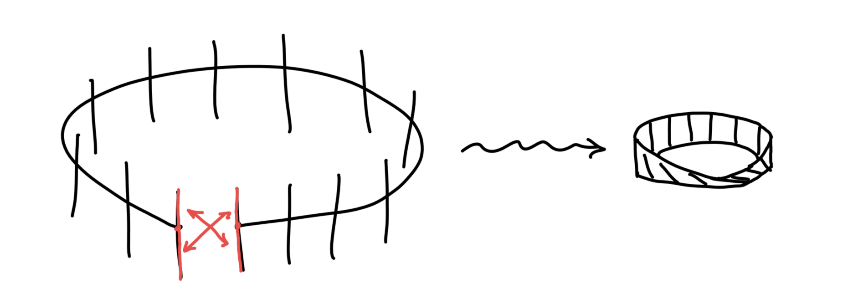
\includegraphics[scale=0.4]{chern_mobius1}
\end{center}

\begin{exercise}
    Check that this defines a vector bundle, by seeing that on an actual open
    cover of $S^1$ we have local trivializations and transition maps, as in the
    following figure.
    \begin{center}
        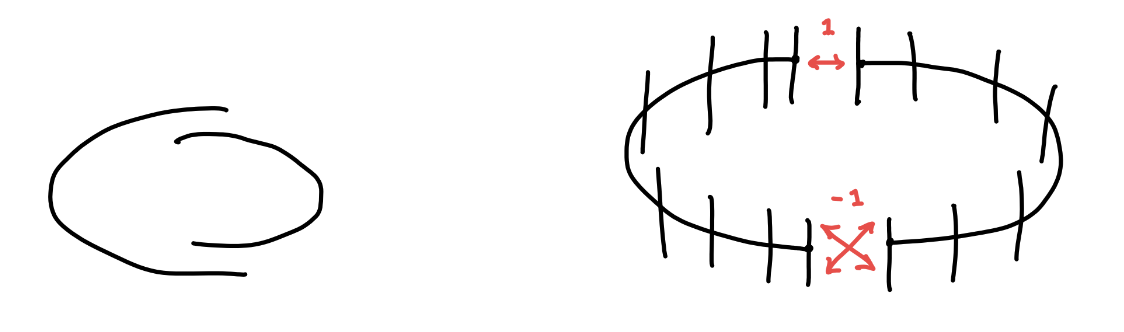
\includegraphics[scale=0.3]{chern_mobius2}
    \end{center}
\end{exercise}

\begin{proof}[Solution]
    With the indicated open cover $S^1=U\cup V$ the intersection $U\cap V$ is a
    disjoint union of two intervals. We glue by $\id$ on one interval and $-\id$
    on the other. This is a locally constant association $U\cap V\to\GL(1,\C)$,
    which is hence continuous.
\end{proof}

\begin{exercise}
    If instead of one twist we include two twists, show that the resulting
    bundle is trivial. Further, show that it can be untwisted to the standard
    band if embedded in $\R^4$.
\end{exercise}

\begin{proof}[Solution]
    If we take two trivializations, where the two twists are contained in one of
    them, then on the two components of the overlap we glue by $\id$ and
    $-(-\id)=\id$, so the trivializations glue to a global trivialization. In
    fact triviality is a consequence of the second part. For the second part,
    note that if we replace one twist of the double-twisted band by the reverse
    oriented twist, then the band can be untwisted to the standard band inside
    $\R^3$:
    \begin{center}
        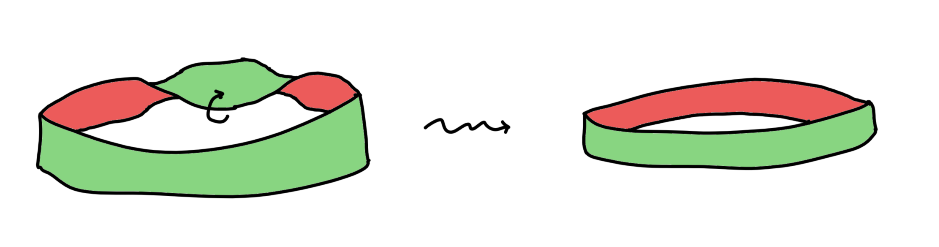
\includegraphics[scale=0.3]{chern_isotopy1}
    \end{center}
    Hence it suffices to show that in $\R^4$ a twist can be reversed. Given a
    twist embedded in $\R^3\times\{0\}\subseteq\R^4$ as pictured below, we can
    achieve this by:
    \begin{itemize}
        \item Perform a straight line isotopy so that the 4th coordinate $x_4$
            is equal to the 2nd coordinate $x_2$.
        \item Perform a straight line isotopy to replace $x_2$ by $-x_2$. This
            leads to no self-intersections since the original coordinates
            can be recovered as $(x_1,x_4,x_3)$.
        \item Perform a straight line isotopy returning $x_4$ to zero. This
            leads to no self-intersections since the original coordinates can
            be recovered as $(x_1,-x_2,x_3)$.
    \end{itemize}
    \begin{center}
        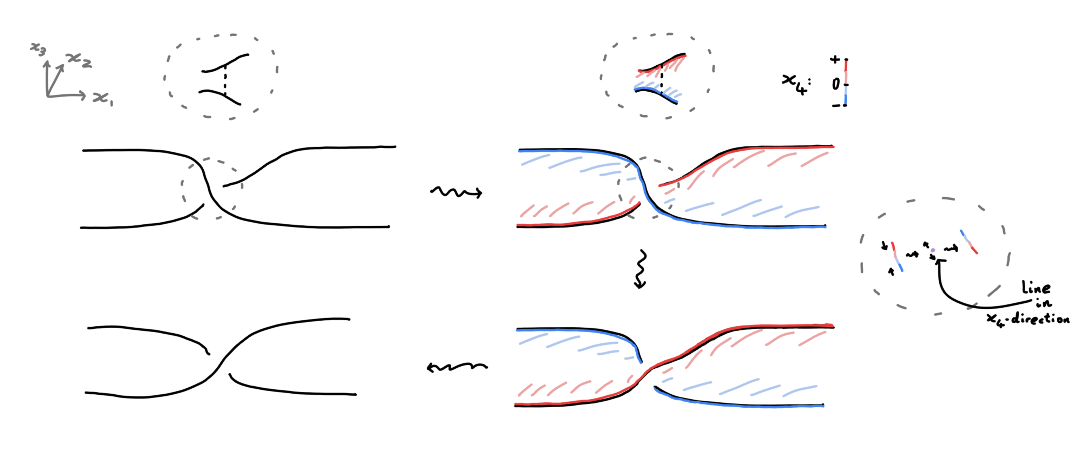
\includegraphics[scale=0.5]{chern_isotopy2}
    \end{center}
\end{proof}

Now we may think of $E$ as $\coprod_U(U\times\C^r)/\sim$, where we glue by the
transition functions $g_{UV}$; for $x\in U\cap V$ we identify
\begin{equation*}
    V\times\C^r\ni(x,e) \sim (x,g_{UV}(x)e)\in U\times\C^r.
\end{equation*}

\begin{exercise}
    Check that this defines an equivalence relation, and that the quotient is
    $E$.
\end{exercise}

\begin{proof}[Solution]
    It is an equivalence relation:
    \begin{itemize}
        \item Reflexive: $(x,e)\sim(x,g_{UU}(x)e)=(x,e)$ as
            $g_{UU}(x)=\id$.
        \item Symmetric: $(x,g_{UV}(x)e)\sim(x,g_{VU}(x)g_{UV}(x)e)=(x,e)$ as
            $g_{VU}(x)\circ g_{UV}(x)=\id$.
        \item Transitive: $(x,e)\sim(x,g_{WV}(x)e)=(x,g_{WU}(x)g_{UV}(x)e)$ as
            $g_{WV}=g_{WU}\circ g_{UV}$.
    \end{itemize}
    We then have a natural map $\coprod_U(U\times\C^r)/\sim\to E$ by the
    universal property of the quotient, which is a homeomorphism over each $U$,
    and a bijection, and therefore a global homeomorphism.
\end{proof}

\begin{exercise}
    Show that the fibres of $\pi$ are naturally vector spaces: if $x_1=(x,e_1)$
    and $x_2=(x,e_2)$ are points of the same fibre $E_x=\pi^{-1}(x)$ and
    $\alpha,\beta\in\C$ we can define $\alpha x_1+\beta x_2\in E_x$ such that...
\end{exercise}

\begin{proof}[Solution]
    In a local trivialization we can take these vector space operations to be
    the natural ones on $\C^r$ under the canonical identification
    $\{x\}\times\C^r\cong\C^r$. This is independent of the choice of local
    trivialization since the vector space operations are preserved by the
    transition maps in $\GL(r,\C)$.
\end{proof}

\begin{exercise}
    Define smooth vector bundles over a smooth manifold, algebraic vector
    bundles over algebraic varieties, real vector bundles, e.t.c.
\end{exercise}

\begin{proof}[Solution]
    For a smooth vector bundle we require the map $U\cap V\to\GL(r,\C)$ to be
    smooth. For an algebraic vector bundle we take local trivializations of the
    form $\pi^{-1}(U)\cong U\times\A^r$, and require $U\cap V\to\GL(r,\C)$ to be
    a regular morphism. For real vector bundles we replace $\C$ by $\R$.
\end{proof}

\paragraph{Sections.} A section of $\pi:E\to X$ is a continuous map $s:X\to E$
such that $\pi\circ s=\id_X$. They form a vector space $\Gamma(E)$ by the
fibre-wise vector space operations.

\begin{exercise}
    A trivialization of the bundle, i.e. an isomorphism
    \begin{equation*}
        \begin{tikzcd}
            &E \ar[d,"\pi"] \ar[r,"\sim"]
                &X\times\C^r \ar[d,"{(x,v)\mapsto x}"] \\
            &X \ar[r,equals] &X
        \end{tikzcd}
    \end{equation*}
    is the same thing as a choice of $r$ sections $s_1,\ldots,s_r$ which form a
    basis at every point, i.e. $s_1(x),\ldots,s_r(x)$ is a basis of $E_x$ for
    every $x\in X$. Hence a trivialization of a line bundle is the same thing as
    a nowhere-vanishing section.
\end{exercise}

\begin{proof}[Solution]
    On a trivial vector bundle $X\times\C^r$ we have a canonical choice of $r$
    sections forming a basis of each fibre given by the basis vectors in $\C^r$;
    every fibre is canonically identified. We can then transport this along the
    isomorphism $E\cong X\times\C^r$ to get such sections for $E$. Conversely,
    given such sections for $E$ we can define an isomorphism
    $E\cong X\times\C^r$ by taking coordinates in $\C^r$ using the basis on each
    fibre.
\end{proof}

\paragraph{Homotopy invariance.} We have
\begin{itemize}
    \item \textbf{Fact 1:} Homotopic bundles are isomorphic. Given
        $E\to X\times[0,1]$, writing $E_t=E|_{X\times\{t\}}$ we have
        $E_0\cong E_1$.

    \item \textbf{Fact 2:} Bundles on contractible spaces $X$ are trivial. If
        $X\simeq\{*\}$ then any bundle $E\to X$ is isomorphic to $X\times\C^r$.
\end{itemize}
For proofs using the Tietze extension theorem see Atiyah's \emph{$K$-Theory}.

So given a rank $r$ bundle $E\to S^n$, we know that restricted to either
hemisphere it is trivial,
\begin{equation*}
    S^n = B^n_1\cup B^n_2, \qquad E|_{B^n_i}\cong B^n_i\times\C^r.
\end{equation*}
These restrictions are glued over the boundary $\partial B^n_i\cong S^{n-1}$ by
a map $S^{n-1}\to\GL(r,\C)$. (Strictly speaking we should take slightly larger
open hemispheres, intersecting in an open annulus which contracts to this
boundary.)

\paragraph{Clutching construction.}

So rank $r$ complex bundles on $S^n$ are in 1-1 correspondence with homotopy
classes of maps $S^{n-1}\to\GL(r,\C)$, i.e. with
\begin{equation*}
    \pi_{n-1}(\GL(r,\C)).
\end{equation*}
E.g. real version with $r=1$ gives
\begin{equation*}
    \{\text{line bundles on $S^1$}\}
        \leftrightarrow \pi_0(\GL(1,\R))
        = \pi_0(\R^\times)
        = \Z/2.
\end{equation*}
(Note that this isn't exactly an example of the previous discussion, since here
the group is disconnected.) This mod 2 integer is the Stiefel--Whitney class of
the bundle.

\paragraph{First Chern class.}
E.g. complex version with $r=1$ gives
\begin{equation*}
    \{\text{line bundles on $S^2$}\}
        \leftrightarrow \pi_1(\GL(1,\C)) = \pi_1(\C^\times) = \Z.
\end{equation*}
This integer classifying the bundle is called its \emph{first Chern class},
$c_1$. For an algebraic version, write
\begin{equation*}
    S^2 \cong \P^1 = \C_x\cup_{\C^\times}\C_y
\end{equation*}
glued over $\C^\times=\{x\ne0\}=\{y\ne0\}$ by $x=\frac{1}{y}$. Then glue trivial
line bundles $\C_x\times\C$ and $\C_y\times\C$ by
\begin{equation*}
    (x,t) \mapsto \biggl(\frac{1}{x},x^{-n}t\biggr) = (y,y^nt).
\end{equation*}
We call the resulting line bundle $\O(n)$ with $c_1=n$.

\paragraph{Tautological bundle.}
When $n=-1$ we get the \emph{tautological bundle} $\O(-1)\to\P^1$. Over $\R$
this is the M\"obius bundle on $\RP^1\cong S^1$:
\begin{center}
    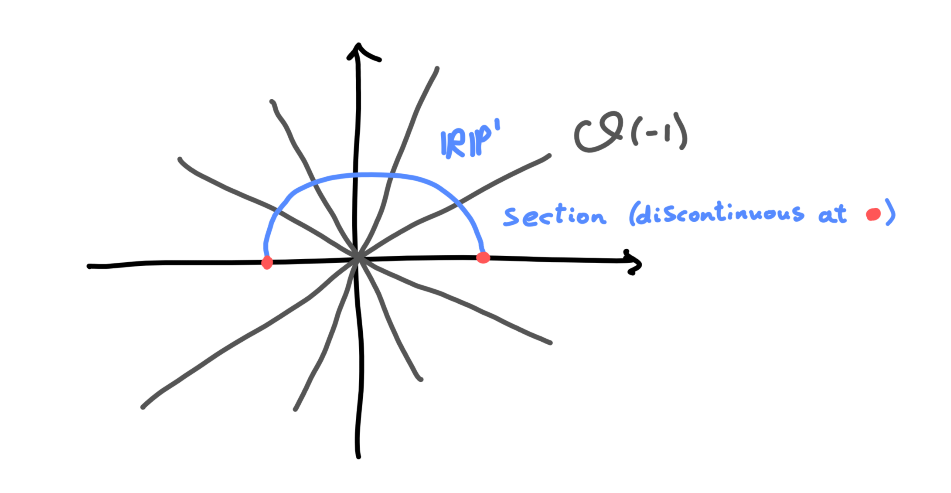
\includegraphics[scale=0.5]{chern_taut1}
\end{center}

\paragraph{Tautological bundle over $\C$.}
Over $\C$ we also see that $\O(-1)$ (defined as above with transition
function $\frac{1}{x}$) is the tautological bundle $\O(-1)$ over $\P^1$.
\begin{center}
    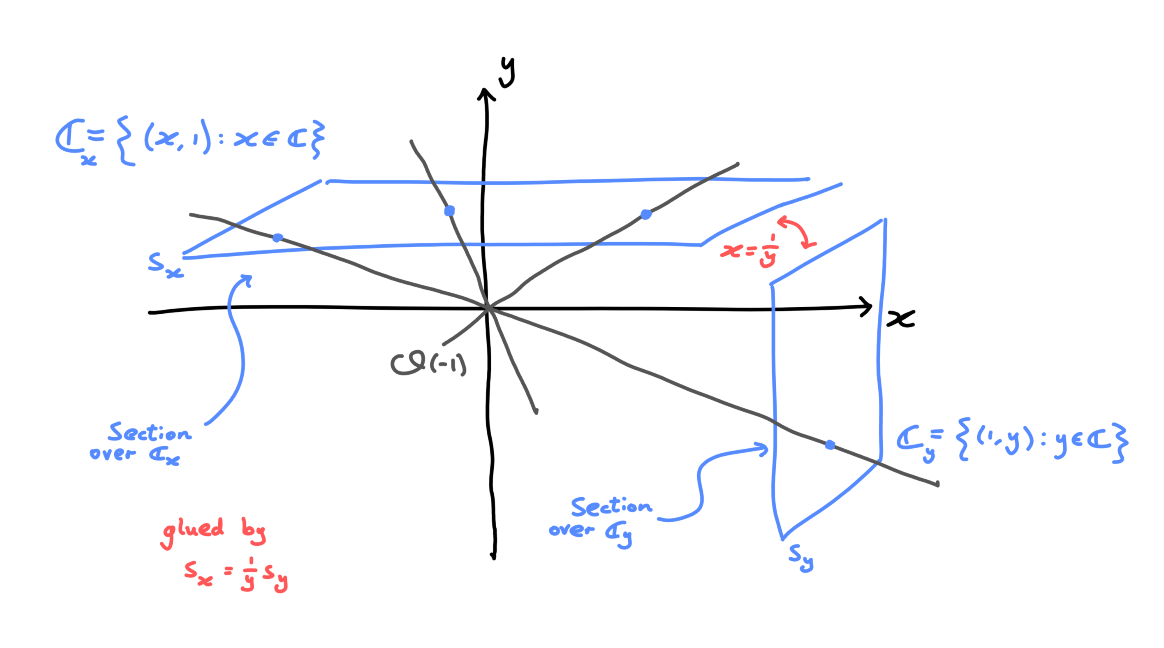
\includegraphics[scale=0.5]{chern_taut2}
\end{center}
We can check that the section $s_x$ when viewed over $\C_y$ does not extend
continuously over the origin, so it doesn't give a trivialization of the whole
bundle.

\paragraph{Zeros of sections.}
The $\O(n)$ line bundle over $\P^1$ was defined with transition function
$x^{-n}$, gluing the section 1 over $\C_x$ to $x^{-n}=y^n$ over $\C_y$. This
therefore defines a \emph{global} holomorphic section of $\O(n)$ when
$n\ge0$, with a degree $n$ zero at $y=0$. (If $n<0$ we get a meromorphic section
with a degree $n$ pole at $y=0$.)

Similarly $p(x)$ over $\C_x$ is glued to $y^np(y^{-1})$ over $\C_y$, so if
$\deg p=n$ we get another algebraic/regular section over $\P^1$. (This gives all
the sections since $\Gamma(\O(n))=\Sym^n(\C^2)^*$.) Again these all have $n$
zeros.

\begin{exercise}
    When $n<0$ we get a meromorphic section with $n$ poles. Instead glue 1 to an
    anti-holomorphic function across the circle $|x|=1$ to give a
    (non-holomorphic) section with $n$ zeros.
\end{exercise}

\begin{proof}[Solution]
    We can glue $1/z^n$ outside the unit circle to $\conj z^n$ inside the unit
    circle, since they agree on the boundary. (If $|z|=1$ then $1/z=\conj z$.)
\end{proof}

\paragraph{Intersection with the zero section.}
Indeed $c_1=n$ is the number of zeros (counted with orientation and
multiplicity) of \emph{any} section of $\O(n)$. In other words, $c_1(L)$ is
the \emph{intersection of the zero section of $L$} with itself (or equivalently
with the graph of any other section).
\begin{center}
    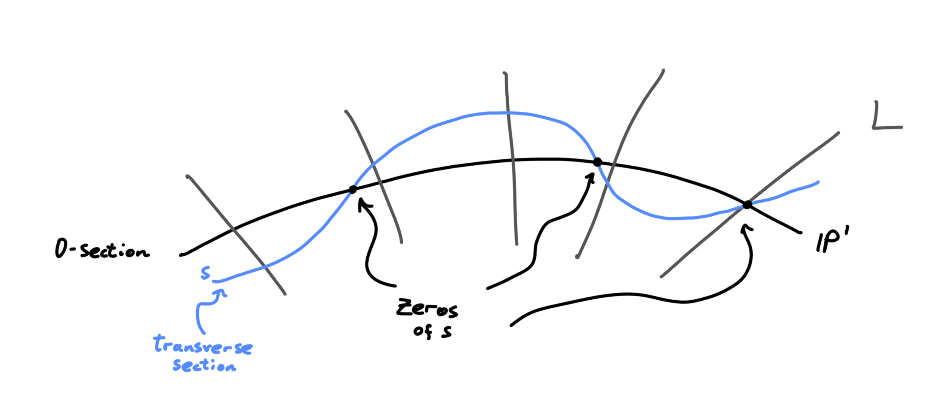
\includegraphics[scale=0.6]{chern_section}
\end{center}

\paragraph{Clutching construction on arbitrary Riemann surfaces.}
Again line bundles are trivial bundles glued across circles / annuli.
\begin{center}
    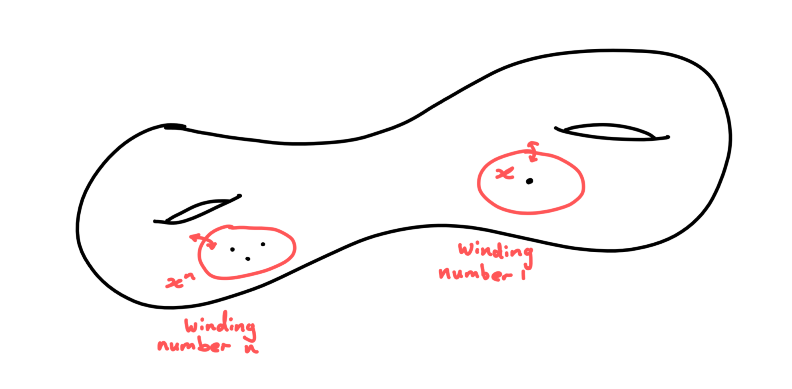
\includegraphics[scale=0.6]{chern_clutch}
\end{center}
\begin{align*}
    c_1(L)
        &= \text{total winding number of transition functions} \\
        &= \text{number of zeros of a section}.
\end{align*}
(So under the line bundle $\leftrightarrow$ divisor correspondence,
$c_1(\O(D))=\deg D$.)

\paragraph{First Chern class on manifolds.}
More generally for any complex line bundle $L$ on a manifold $M$ we define
\begin{equation*}
    c_1(L) = [s^{-1}(0)]\in H_{\dim X-2}(X)
\end{equation*}
where $s$ is any section \emph{transverse to the zero section}. (If $s'$ is
another choice then we have a homotopy $s_t=(1-t)s+ts'$ so that $s_t^{-1}(0)$ is
a chain interpolating from $s$ to $s'$.)

In fact we can define $c_1(L)$ to be the Poincar\'e dual of $[s^{-1}(0)]$, as
this cohomology class will generalize to arbitrary topological spaces $X$. For
general $X$ we can understand $c_1(L)\in H^2(X)$ by evaluating it on
$[\Sigma]\in H_2(X)$ for Riemann surfaces $\Sigma\hookrightarrow X$, by
\begin{equation*}
    \langle c_1(L),[\Sigma]\rangle = c_1(L|_\Sigma).
\end{equation*}

\paragraph{Higher Chern classes on manifolds.}
For any rank $r$ complex vector bundle $E\to X$ pick a transverse
$C^\infty$-section $s$ and define the \emph{Euler class} or top Chern class
\begin{equation*}
    e(E) = c_r(E) = [s^{-1}(0)] \in H_{\dim X-2r}(X) \cong H^{2r}(X).
\end{equation*}
Analogously define
\begin{equation*}
    c_k(E) \in H^{2k}(X)
\end{equation*}
to be Poincar\'e dual to the locus where $r-k+1$ generic sections fail to be
linearly independent:
\begin{equation*}
    [(s_1\wedge\cdots\wedge s_{r-k+1})^{-1}(0)] \in H_{\dim X-2}(X).
\end{equation*}
So $c_r(E)=e(E)$ while $c_1(E)=c_1(\Lambda^rE)$ and $c_i(E)=0$ for $i>r$.
(When $k\ne1,r$ note that $c_k(E)\ne e(\Lambda^{r-k+1}E)$---this has the wrong
degree, and $s_1\wedge\cdots\wedge s_{r-k+1}$ is \emph{not} a generic section of
$\Lambda^{r-k+1}E$.)

\paragraph{Whitney sum formula.}
Given two generic sections $s_1\in\Gamma(E_1)$, $s_2\in\Gamma(E_2)$ where $E_i$
has rank $r_i$, we get a section $s_1\oplus s_2\in\Gamma(E_1\oplus E_2)$, with
\begin{equation*}
    e(E_1\oplus E_2)
        = [(s_1\oplus s_2)^{-1}(0)]
        = [s_1^{-1}(0)\cap s_2^{-1}(0)]
        = e(E_1)\cup e(E_2) \in H^{2r_1+2r_2}.
\end{equation*}
In particular, for line bundles
$c_2(L_1\oplus L_2)=c_1(L_1)\cup c_1(L_2)$ and
\begin{align*}
    c_1(L_1\oplus L_2)
        &= c_1(\Lambda^2(L_1\oplus L_2)) \\
        &= c_1(L_1\otimes L_2) \\
        &= [(s_1\otimes s_2)^{-1}(0)] \\
        &= [s_1^{-1}(0)\cup s_2^{-1}(0)] \\
        &= c_1(L_1) + c_1(L_2).
\end{align*}
We can write this as $c(L_1\oplus L_2)=c(L_1)\cup c(L_2)$ where the
\emph{total Chern class} is defined as
\begin{equation*}
    c(E)=1+c_1(E)+c_2(E)+\cdots\in H^*(X).
\end{equation*}
More generally, for bundles $E,F$ of rank $r,s$ use the decomposition
\begin{equation*}
    \Lambda^k(E\oplus F) = \bigoplus_{i=0}^k\Lambda^i(E)\otimes\Lambda^{k-i}(F)
\end{equation*}
and generic sections $e_1,\ldots,e_k\in\Gamma(E)$ and
$f_1,\ldots,f_k\in\Gamma(F)$ to compute
\begin{align*}
    \bigl[\bigl(&(e_1\wedge\cdots\wedge e_k)
        \oplus(e_1\wedge\cdots\wedge e_{k-1}\otimes f_k)
        \oplus\cdots \\
           &\qquad\oplus(e_1\otimes f_2\wedge\cdots\wedge f_k)
           \oplus(f_1\wedge\cdots\wedge f_k)
       \bigr)^{-1}(0)\bigr].
\end{align*}

\begin{exercise}
    Work it out and take Poincar\'e duals to give
    \begin{equation*}
        c_{r+s-k+1}(E\oplus F)
            = c_r(E)c_{s-k+1}(F) + \cdots + c_{r-k+1}(E)c_s(F).
    \end{equation*}
    Deduce the \emph{Whitney sum formula} $c(E\oplus F)=c(E)c(F)$.
\end{exercise}

\begin{proof}[Solution]
    For the given definition of $c_{r+s-k+1}(E\oplus F)$, we take generic
    sections $e_1\oplus f_1,\ldots,e_k\oplus f_k$ of $E\oplus F$, and consider
    their wedge product. Under the decomposition
    $\Lambda^k(E\oplus F)=\bigoplus_{i=0}^k\Lambda^i(E)\otimes\Lambda^{k-i}(F)$
    this is given by
    \begin{align*}
        (e_1\oplus f_1)\wedge\cdots\wedge(e_k\oplus f_k)
            &= (e_1\wedge\cdots\wedge e_k)
                \oplus(e_1\wedge\cdots e_{k-1}\otimes f_k)
                \oplus\cdots \\
            &\qquad\oplus(e_1\otimes f_2\wedge\cdots\wedge f_k)
                \oplus(f_1\wedge\cdots\wedge f_k),
    \end{align*}
    and $c_{r+s-k+1}(E\oplus F)$ is represented by the Poincar\'e dual of the
    vanishing locus of this section.

    \textbf{Set-theoretical Claim:} Given a set $S$ with chains of subsets
    \begin{equation*}
        A_0\subseteq A_1\subseteq\cdots\subseteq A_k=S
        \quad\text{and}\quad
        S=B_0\supseteq B_1\supseteq\cdots\supseteq B_k,
    \end{equation*}
    we have
    \begin{equation*}
        \bigcap_{i=0}^k(A_i\cup B_i)
            = \bigcup_{j=1}^k(A_j\cap B_{j-1}).
    \end{equation*}

    Applying this to the subsets $A_i=(e_1\wedge\cdots\wedge e_i)^{-1}(0)$,
    $B_i=(f_{i+1}\wedge\cdots\wedge f_k)^{-1}(0)$ of $X$, we get
    \begin{align*}
        &\bigl[(e_1\wedge\cdots\wedge e_k)^{-1}(0)
            \cap(e_1\wedge\cdots\wedge e_{k-1}\otimes f_k)^{-1}(0)
            \cap\cdots \\
        &\qquad\qquad\cap(e_1\otimes f_2\wedge\cdots\wedge f_k)^{-1}(0)
            \cap(f_1\wedge\cdots\wedge f_k)^{-1}(0)
        \bigr] \\
        &\qquad=\biggl[\bigcap_{i=0}^k
            \bigl((e_1\wedge\cdots\wedge e_i)^{-1}(0)
        \cup(f_{i+1}\wedge\cdots\wedge f_k)^{-1}(0)\bigr)\biggr] \\
        &\qquad=\biggl[\bigcup_{j=1}^k
            \bigl((e_1\wedge\cdots\wedge e_j)^{-1}(0)
            \cap(f_j\wedge\cdots\wedge f_k)^{-1}(0)\bigr)\biggr], \\
    \end{align*}
    and hence
    \begin{align*}
        c_{r+s-k+1}(E\oplus F)
            &= \sum_{j=1}^kc_{r-j+1}(E)c_{s-k+j}(F) \\
            &= c_r(E)c_{s-k+1}(F) + \cdots + c_{r-k+1}(E)c_s(F).
    \end{align*}
\end{proof}

\paragraph{Axiomatic approach.}

\begin{fact}
    Knowing (or defining!) $c_1(\O_{\P^n}(1))=[\P^{n-1}]$, the Whitney sum
    formula and functoriality is then enough to completely determine all Chern
    classes on all topological spaces.
\end{fact}

Functoriality: $c(f^*E)=f^*c(E)$.

\begin{exercise}
    Define $f^*E$ and prove this using zero loci of sections when $f:X\to Y$ is
    a map of manifolds.
\end{exercise}

\begin{proof}[Solution]
    Given local trivializations $E|_U\cong U\times\C^r$, we define a local
    trivialization $f^*E|_{f^{-1}(U)}\cong f^{-1}(U)\times\C^r$ by associating
    $(x,v)\in f^{-1}(U)\times\C^r$ with $(f(x),v)\in U\times\C^r$. The
    transition functions are given by the transition functions for $E$ composed
    with $f$, and hence remain continuous, so this defines a vector bundle. Then
    if $s_1,\ldots,s_k$ are generic sections of $E$, we get that
    $f^*s_1,\ldots,f^*s_k$ are generic sections of $f^*E$ since all sections of
    $f^*E$ are pullbacks of sections of $E$. (Assuming $X$ and $Y$ are compact,
    so $f$ is closed.) Moreover the vanishing locus of
    $f^*s_1\wedge\cdots\wedge f^*s_k=f^*(s_1\wedge\cdots\wedge s_k)$ is the
    preimage under $f$ of the vanishing locus of $s_1\wedge\cdots\wedge s_k$.
    Since the cohomology class of the preimage gives the pullback of the
    cohomology class (for suitably general representatives missing critical
    values of $f$) this shows naturality of the Chern class.
\end{proof}

There are two steps to proving this fact:
\begin{itemize}
    \item All rank $r$ bundles on $X$ are pullbacks $f^*Q$ of the
        \emph{universal bundle on the classifying space} $Q\to B\GL(r,\C)$ by a
        map $f:X\to B\GL(r,\C)$. (So we only need to define $c_i$ on one
        classifying space.)

    \item Splitting principle: We may assume $E$ is a direct sum of line bundles
        without loss of generality.
\end{itemize}

\paragraph{Classifying space.}
Any bundle $E$ is a quotient of an infinite rank trivial bundle
$\underline{\Gamma(E)}$ (here $\underline V$ denotes the trivial bundle with
fibre $V$):
\begin{equation*}
    \underline{\Gamma(E)} \xrightarrow{\ev} E\to 0. \tag{$*$}
\end{equation*}
(Or take a sufficiently large subbundle
$\underline\C^N\subseteq\underline\C^\infty=\underline{\Gamma(E)}$, $N\gg0$.)
Therefore it defines a map from $X$ to the Grassmannian
\begin{align*}
    f:X&\to\Gr(\C^\infty,r), \\
    x &\mapsto (*)_x.
\end{align*}
There is a tautological universal quotient bundle $Q\to\Gr(\C^\infty,r)$
\begin{equation*}
    \underline\C^\infty \to Q \to 0 \qquad \text{over $\Gr(\C^\infty,r)$,}
\end{equation*}
and from ($*$) we get that $f$ pulls this back to give $E$; $f^*Q\cong E$. Thus
$\Vect_r(X)=[X,\Gr(\C^\infty,r)]$. We call $\Gr(\C^\infty,r)$ the
\emph{classifying space} $B\GL(r,\C)$. For example, if $r=1$ we have
$B\C^\times=\CP^\infty$, so any line bundle $\L\to X$ is $f^*\O(1)$ for some
(homotopy class of) map $f:X\to\CP^\infty$ (or $f:X\to\CP^N$ for $N\gg0$ if $X$
is finite dimensional). Then
\begin{equation*}
    c_1(\L) = f^*c_1(\O(1)) = f^*h
\end{equation*}
where $h\in H^2(\CP^\infty)$ is the generator (the limit as $N\to\infty$ of the
Poincar\'e duals of $\CP^{N-1}\subseteq\CP^N$, or the standard K\"ahler form).

\paragraph{Splitting principle.}
Given $E\to X$ (e.g. $Q\to\Gr(\C^\infty,r)$) there is a space dominating $X$ on
which $E$ splits as a sum of line bundles:
\begin{equation*}
    \pi:Y\to X \quad \text{such that} \quad \pi^*E=\L_1\oplus\cdots\oplus\L_r,
\end{equation*}
with fibres $Y_x=\pi^{-1}(x)$ given by the flag manifolds
\begin{equation*}
    Y_x = \{\text{linearly independent complex line bundles
        $L_1,\ldots,L_r\subseteq E_x$}\}.
\end{equation*}
There are universal / tautological bundles $\L_i$ on $Y$, and it is then
tautological that $\pi^*E\cong\oplus_{i=1}^r\L_i$.

\textbf{Fact:} $\pi^*:H^*(X)\to H^*(Y)$ is an injection, so pulling back $c(E)$
loses no information, and
\begin{equation*}
    \pi^*c(E) = c(\pi^*E) = c(\L_1\oplus\cdots\oplus\L_r)
        = c(\L_1)\cdots c(\L_r).
\end{equation*}
Hence for $E\to X$ we get a diagram
\begin{equation*}
    \begin{tikzcd}
        &Y \ar[r,"f"] \ar[d,"\pi"] &B(\C^\times)^r = (\CP^\infty)^r \\
        &X
    \end{tikzcd}
\end{equation*}
such that $\pi^*:H^*(X)\to H^*(Y)$ is an injection, and $c(E)\in H^*(X)$ is the
unique class such that
\begin{equation*}
    \pi^*c(E) = f^*[(1+h_1)\cdots(1+h_r)].
\end{equation*}
So the splitting principle, the Whitney sum formula, and $c_1(\O(1))=h$
determine all Chern classes uniquely. (Existence takes a little bit more work,
e.g. computing $H^*(\Gr(\C^\infty,r))$.)

\begin{exercise}
    Prove the following corollary: If $E$ has rank $r$, then $c_i(E)=0$ for
    $i>r$.
\end{exercise}

\begin{proof}[Solution]
    From above we have
    \begin{equation*}
        \pi^*c(E) = (1+f^*h_1)\cdots(1+f^*h_r)
    \end{equation*}
    where $h_1,\ldots,h_r$ have degree 1, so the RHS has no terms in degree
    $i>r$. Hence $\pi^*c_i(E)=0$, and since $\pi^*$ is injective $c_i(E)=0$.
\end{proof}

\paragraph{Grothendieck's definition.}
On the projective bundle $\pi:\P(E)\to X$ we have the tautological inclusion
\begin{equation*}
    \O_{\P(E)}(-1) \hookrightarrow \pi^*E.
\end{equation*}
Since the quotient bundle is of rank $r-1$,
\begin{equation*}
    c_r(\pi^*E/\O_{\P(E)}(-1)) = 0.
\end{equation*}
By the Whitney sum formula, this is the degree $r$ part of
\begin{equation*}
    \pi^*c(E)/c(\O_{\P(E)}(-1)) = \pi^*c(E)/(1-h),
\end{equation*}
where $h=c_1(\O_{\P(E)}(-1))$. Thus
\begin{equation*}
    h^r + \pi^*c_1(E)h^{r-1} + \cdots + \pi^*c_{r-1}(E)h + \pi^*c_r(E) = 0.
        \tag{$*$}
\end{equation*}
\textbf{Fact:} $H^*(\P(E))
=H^*(X)\oplus H^*(X)h\oplus\cdots\oplus H^*(X)h^{r-1}$, so $h^r$ can be uniquely
written as a linear combination of $1,h,\ldots,h^{r-1}$ and we can define
$c_i(E)$ via ($*$).

\paragraph{Chern--Weil for line bundles.}
If $X$ is a manifold we can pick a connection $A$ on $\L\to X$. Its curvature
$F_A$ is a closed 2-form; $dF_A=0$. Changing $a\mapsto A+a$ gives
$F_A\mapsto F_A+da$, so $[F_A]\in H^2(X;\R)$ is independent of $A$. In fact it
is given by
\begin{equation*}
    \frac{[F_A]}{2\pi i} = [c_1(\L)] \in H^2(X;\Z)/\text{torsion}.
\end{equation*}
Let's prove this for $X$ a Riemann surface and $\L$ described by the clutching
construction. Write $X=U\cup_{S^1}D^2$ where $D^2$ is a disc and $S^1$ is an
annulus thickening its boundary. Write $\L$ as
$\underline\C_U\cup_\phi\underline\C_{D^2}$ for a transition function
$\phi:S^1\to\C^\times$ of winding number $n=c_1(\L)$. Put the trivial connection
$d$ on $\underline\C_U$. In the trivialization $\underline\C_D$ restricted to
the annulus this is the connection
\begin{equation*}
    d+\phi^{-1}d\phi
\end{equation*}
since this annhilates $\phi$ (which is glued to 1 on $U$). Extend this to any
connection $d+a$ over $D^2$ and compute
\begin{align*}
    \int_XF_A = \int_{D^2}F_A = \int_{D^2}da = \int_{S^1}da
              = \int_{S^1}\frac{d\phi}{\phi} = \int_{S^1}d\log\phi
              = 2\pi in.
\end{align*}

\paragraph{Chern--Weil theory.}
Suppose $X$ is a manifold with a rank $r$ bundle $E\to X$ and a connection $A$
on $E$. Form
\begin{equation*}
    p\biggl(\frac{F_A}{2\pi i}\biggr) \in H^{2k}(X;\R)
\end{equation*}
for any ad-invariant ($p(N^{-1}MN)=p(M)$) polynomial function $p$ of
$\End(\C^r)$. For example $p$ could be $\tr$ (giving $c_1(E)$), or $\det$
(giving $c_r(E)$), or any other symmetric polynomial in the eigenvalues. (In
fact $H^*(B\GL(r,\C))=\text{Ad-invariant polynomials}$.) If $p$ is integral, the
result is an integral characteristic class.

\begin{exercise}
    Show that $p(F_A)$ is closed, and changes by an exact form under
    $A\mapsto A+a$.
\end{exercise}

\begin{theorem}
    We have $c(E)=\det(\id+\frac{F_A}{2\pi i})$ in $H^*(X)/\text{torsion}$, i.e.
    \begin{equation*}
        1 + c_1(E) + c_2(E) + \cdots
            = 1 + \frac{\tr F_A}{2\pi i} - \frac{\tr(F_A\wedge F_A)}{4\pi^2}
                + \cdots.
    \end{equation*}
\end{theorem}

\paragraph{Tangent bundle to projective space.}
Let $V=\C^{n+1}$ so that $\P(V)=\P^n$. Then
\begin{equation*}
    T_{\P^n} = \O(-1)^*\otimes\underline V/\O(-1).
\end{equation*}
\begin{proof}[Sketch]
    A point of $\P(V)$ is a complex line $L\le V$. Pick any complement to write
    $V=L\oplus V/L$. Then nearby lines in $V$ are graphs of linear maps
    $L\to V/L$. So the tangent space is $L^*\otimes V/L$.
\end{proof}
\begin{center}
    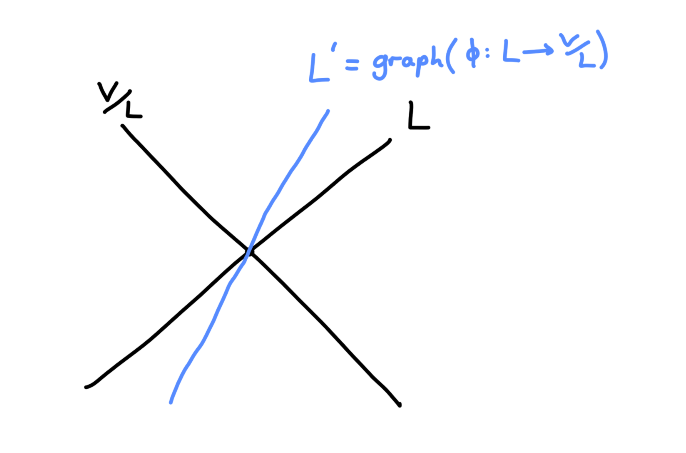
\includegraphics[scale=0.4]{chern_tangent}
\end{center}

\paragraph{Chern classes of projective space.}
Applying the Whitney sum formula to $T_{\P^n}=\underline V(1)/\O(-1)$ gives
\begin{equation*}
    c(T_{\P^n})
        = c(\underline V(1))/c(\O(-1))
        = c(\O(1)^{\oplus(n+1)})
        = (1+h)^{n+1},
\end{equation*}
where $h=c_1(\O(1))$ is the hyperplane class Poincar\'e dual to
$\P^{n-1}\subseteq\P^n$. (So for example $c_n(T_{\P^n})=(n+1)h^n$, and
integrating gives $e(\P^n)=n+1$.)

\paragraph{Hypersurfaces in projective space.}
\begin{exercise}
    ``Adjunction'': If $s\in\Gamma(E)$ is transverse to the zero section, show
    its zero locus $Z=s^{-1}(0)$ has normal bundle $N_{Z/X}=E|_Z.$
    \begin{center}
        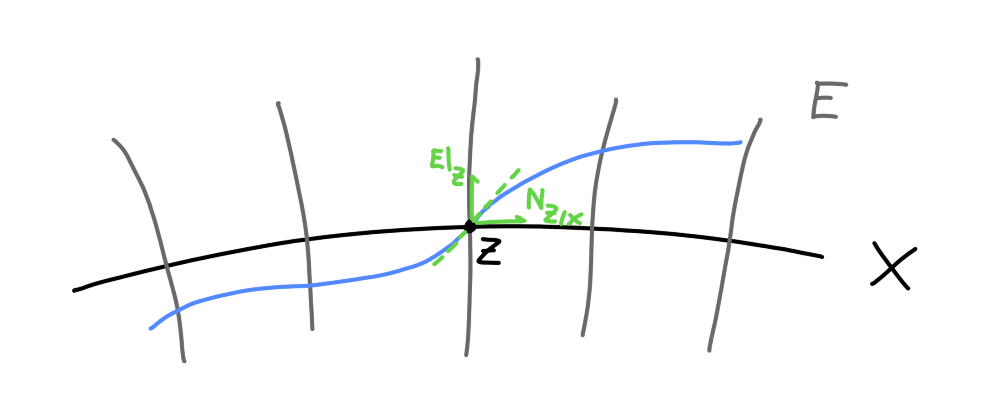
\includegraphics[scale=0.5]{chern_normal}
    \end{center}
\end{exercise}

\begin{proof}[Solution]
    Note that $TE=\pi^*(TX\oplus E)$, and so the derivative of $s$ gives a map
    \begin{equation*}
        TX\to s^*TE = s^*\pi^*(TX\oplus E) = TX\oplus E
    \end{equation*}
    whose projection to $TX$ is the identity. The condition of being transverse
    to the zero section means that the projection to $E$ is non-zero over $Z$.
    Furthermore, note that $TX|_Z=TZ\oplus N_{Z/X}$, and the derivative of $s$
    vanishes on $TZ$ since $s|_Z=0$. Therefore the composite
    \begin{equation*}
        TZ\oplus N_{Z/X} = TX|_Z \to TX|_Z\oplus E|_Z \to E|_Z
    \end{equation*}
    vanishes on $TZ$, but is non-zero and hence induces an isomorphism
    $N_{Z/X}\to E|_Z$ of line bundles.
\end{proof}

\begin{exercise}
    Hence work out the total Chern class $c(T_{X_d})$ of a degree $d$
    hypersurface $X_d\subseteq\P^n$ (the zero locus of a section of $\O(d)$).
    Apply to $n=3$, $d=4$ to find $c_1(T_S)$ and $e(S)$ for $S$ a ``K3
    surface''.
\end{exercise}

\begin{proof}[Solution]
    Let $i:X_d\hookrightarrow\P^n$ denote the inclusion. Note that
    $i^*T_{\P^n}=T_{X_d}\oplus N_{X_d/\P^n}$, so by the Whitney sum
    formula
    \begin{equation*}
        c(T_{X_d}) = c(i^*T_{\P^n})/c(N_{X_d/\P^n}).
    \end{equation*}
    But from naturality of the Chern class, and the above computation of
    $c(T_{\P^n})$, we have
    \begin{equation*}
        c(i^*T_{\P^n}) = i^*(1+h)^{n+1} = (1+\omega)^{n+1},
    \end{equation*}
    where $\omega=i^*h$. Moreover the previous exercise gives
    $N_{X_d/\P^n}\cong i^*\O(d)$, so by naturality and the Whitney sum formula
    \begin{equation*}
        c(N_{X_d/\P^n})
            = c(i^*\O(d))
            = i^*(1+c_1(\O(1)^{\otimes d}))
            = (1+d\cdot\omega).
    \end{equation*}
    Hence
    \begin{equation*}
        c(T_{X_d}) = (1+\omega)^{n+1}/(1+d\cdot\omega).
    \end{equation*}
    When $n=3$ and $d=4$ we have $\omega^3=0$, and
    \begin{align*}
        c(T_S)
            &= (1+\omega)^4/(1+4\omega) \\
            &= (1+4\omega+6\omega^2)(1-4\omega+16\omega^2) \\
            &= 1+6\omega^2.
    \end{align*}
    Hence $c_1(T_S)=0$ and $e(T_S)=6\omega^2$.
\end{proof}

\begin{exercise}
    Compute $c_i(\End(E))$ in terms of $c_i(E)$ for $E$ a rank 2 bundle. (Hint:
    Splitting principle.) Why did you find $c_1=0=c_3=c_4$?
\end{exercise}

\begin{proof}[Solution]
    First assume $E=L_1\oplus L_2$ is a sum of line bundles. Then
    $\End(E)=\bigoplus_{i,j}L_i^*\otimes L_j$, so by the Whitney sum formula
    \begin{align*}
        c(\End(E))
            &= \prod_{i,j}c(L_i^*\otimes L_j) \\
            &= \prod_{i,j}(1 + c_1(L_j) - c_1(L_i)) \\
            &= 1 + 2c_1(L_1)c_1(L_2) - c_1(L_1)^2 - c_1(L_2)^2 \\
            &= 1 + 4c_2(E) - c_1(E)^2.
    \end{align*}
    This then holds in general by the splitting principle and the naturality of
    the Chern class. We get that the only non-vanishing Chern class of $\End(E)$
    is $c_2(\End(E))=4c_2(E)-c_1(E)^2$.
\end{proof}

\begin{exercise}
    ~
    \begin{enumerate}[label=(\arabic*)]
        \item Compute $c_4(\Sym^3(E))$ in terms of $c_i(E)$ for $E$ a rank 2
            bundle. (Hint: Splitting principle.)

        \item The Grassmannian $\Gr(2,\C^4)$ of 2-planes in $\C^4$ has a
            universal subbundle $\U\hookrightarrow\underline\C^4$. Describe a
            cycle Poincar\'e dual to $c_2(\U^*)$. (Hint: Use
            $(\underline\C^4)\twoheadrightarrow\U^*$ to pick a section of
            $\U^*$.)

        \item Describe a cycle Poincar\'e dual to $c_1(\U^*)$. (Hint: Pick two
            sections of $\U^*$ and see where they're linearly dependent.)
    \end{enumerate}
\end{exercise}

\begin{proof}[Solution]
    \begin{enumerate}[label=(\arabic*)]
        \item By the splitting principle and naturality we may assume
            $E=L_1\oplus L_2$ is a sum of line bundles. Then
            \begin{equation*}
                \Sym^3(E) = \bigoplus_{k=0}^3
                    \bigl(L_1^{\otimes k}\otimes L_2^{\otimes(3-k)}\bigr),
            \end{equation*}
            so by the Whitney sum formula
            \begin{equation*}
                c(\Sym^3(E))
                    = \prod_{k=0}^3\bigl(1 + kc_1(L_1) + (3-k)c_1(L_2)\bigr).
            \end{equation*}
            Writing $\gamma_i=c_1(L_i)$, we then have
            \begin{align*}
                c_4(\Sym^3(E))
                    &= 9\gamma_1\gamma_2
                        (\gamma_1+2\gamma_2)(2\gamma_1+\gamma_2) \\
                    &= 9\gamma_1\gamma_2
                        \bigl(2(\gamma_1+\gamma_2)^2 + \gamma_1\gamma_2\bigr) \\
                    &= 18c_2(E)c_1(E)^2 + 9c_2(E)^2.
            \end{align*}

        \item The class $c_2(\U^*)$ is Poincar\'e dual to the vanishing locus of
            a generic section of $\U^*$. Using the inner product on $\C^4$ we
            have a decomposition $\C^4=\U\oplus\U^*$, and then a generic section
            of $\U^*$ is the image $\langle v,-\rangle$ of a generic section $v$
            of $\underline\C^4$. The vanishing locus of this section is the set
            of planes perpendicular to a continuously varying vector, which if
            we take a constant vector gives $\Gr(2,\C^3)\subseteq\Gr(2,\C^4)$.

        \item Taking two sections $\langle v_1,-\rangle$ and
            $\langle v_2,-\rangle$ of $\U^*$, they are linearly dependent at the
            planes whose orthogonal complements intersect the span
            $\langle v_1,v_2\rangle$. Swapping with orthogonal complements we
            then see that $c_1(\U^*)$ is Poincar\'e dual to the cycle given by
            those planes intersecting $\C^2\subseteq\C^4$ in $\Gr(2,\C^4)$.
    \end{enumerate}
\end{proof}

\begin{exercise}
    Using (1,2,3) above, show that $\int_{\Gr(2,\C^4)}c_4(\Sym^3\U^*)=27$.
\end{exercise}

\begin{proof}[Solution]
    Note that the self-intersection of the cycle Poincar\'e dual to $c_2(\U^*)$
    from (2) is the intersection $\Gr(2,V)\cap\Gr(2,W)=\Gr(2,V\cap W)$ for
    generic 3-dimensional subspaces $V,W\subseteq\C^4$. Now generically
    $\dim(V\cap W)=2$, so this is a single point. Hence $c_2(\U^*)^2$ is
    Poincar\'e dual to the cycle represented by a point, i.e. it is the standard
    generator $\omega\in H^4(\Gr(2,\C^4))$. Also, the self-intersection of the
    cycle Poincar\'e dual to $c_1(\U^*)$ from (3) is represented by the planes
    intersecting two generic copies of $\C^2$ in $\C^4$, which are the sums of
    lines in $\C^2$ with lines in a chosen complement of $\C^2$. Intersecting
    this with the cycle Poincar\'e dual to $c_2(\U^*)$ from (2) gives a point,
    since a generic copy of $\C^3$ intersects both copies of $\C^2$ in a line.
    Hence $c_2(\U^*)c_1(\U^*)^2$ is also $\omega$, and we get
    \begin{equation*}
        \int_{\Gr(2,\C^4)}c_4(\Sym^3\U^*)
            = \int_{\Gr(2,\C^4)}(18\omega+9\omega)
            = 27\int_{\Gr(2,\C^4)}\omega
            = 27
    \end{equation*}
    since the integral of $\omega$ is the intersection number of $\Gr(2,\C^4)$
    with a point, which is 1.
\end{proof}

\begin{exercise}
    Identify $\Gr(2,\C^4)$ with $\{\text{lines $\P^1\subseteq\P^3$}\}$. Let
    $s\in\Gamma(\O_{\P^3}(3))$ cut out a cubic surface $S\subseteq\P^3$. Show
    that $s$ defines a section of $\Sym^3\U^*$ over $\Gr(2,\C^4)$ cutting out
    the lines in $\P^3$ which lie in $S$, of which there are hence 27.
\end{exercise}

\begin{proof}[Solution]
    Pulling back $s$ gives a section of $\O_{\P^1}(3)$ for each line
    $\P^1\subseteq\P^3$. Now $\O_{\P(V)}(d)\cong\Sym^dV^*$, both having bases
    given by monomials, so from this we get a section of $\Sym^3\U^*$ since each
    $\P^1$ corresponds to the projectivization of the associated fibre of $\U$.
    This section vanishes when the homogeneous polynomial defining $s$
    restricted to the line $\P^1$ is zero, i.e. when the line $\P^1$ lies in
    $S$. The Poincar\'e dual of this vanishing locus is $c_4(\Sym^3\U^*)$, so by
    the previous exercise the number of such lines is 27. (Assuming $S$ is
    smooth, so that $s$ is transverse to the zero section.)
\end{proof}

\paragraph{Segre classes.}
We defined $c_i(E)$ as (Poincar\'e dual to) the locus where $r-i+1$ generic
sections fail to be linearly independent, i.e. the $x\in X$ s.t.
\begin{equation*}
    \C^{r-i+1} \xrightarrow{s_1(x),\ldots,s_{r-i+1}(x)}E_x
\end{equation*}
fails to be injective. Similarly, we can define the $i$th \emph{Segre class}
$s_i(E)\in H^{2i}(X)$ to be ($(-1)^i$ times the Poincar\'e dual of) the locus
where $r+i-1$ generic sections fail to generate $E$, i.e. the $x\in X$ s.t.
\begin{equation*}
    \C^{r+i-1}\xrightarrow{s_1(x),\ldots,s_{r+i-1}(x)}E_x
\end{equation*}
fails to be surjective.

\begin{exercise}
    Show that for line bundles $s_i(\L)=(-1)^ic_1(\L)^i$.
\end{exercise}

\begin{proof}[Solution]
    When $r=1$, a collection of $r+i-1=i$ generic sections fails to generate the
    line bundle only at the points where they all vanish. Each individual
    vanishing locus represents $c_1(\L)$, so the intersection represents
    $c_1(\L)^i$.
\end{proof}

In fact $s(E)=c(E)^{-1}$, where $s(E)=1+s_1(E)+s_2(E)+\cdots\in H^*(X)$.

\paragraph{\v{C}ech cohomology formulation.}
Let $\O$ denote the sheaf of (holomorphic, algebraic, $C^\infty$, or ...)
functions, and $\O^\times$ the (multiplicative) sheaf of invertible functions.
Then the exact sequence (in Euclidean topology)
\begin{equation*}
    0\to\underline\Z\xrightarrow{2\pi i}\O\xrightarrow\exp\O^\times\to1
\end{equation*}
induces the long exact sequence of \v{C}ech cohomology groups
\begin{equation*}
    H^1(X,\O^\times) \xrightarrow\delta H^2(X,\Z) \to H^2(X,\O).
\end{equation*}
Consider an element $e\in H^1(X,\O^\times)$ (i.e. invertible $e_{UV}$ on each
overlap $U\cap V$ satisfying $e_{UV}e_{VW}e_{UW}=1$ on $U\cap V\cap W$) to be
the transition functions for a line bundle $\L$.

\begin{exercise}
    Identify $\delta(e)\in H^2(X,\Z)$ with $c_1(\L)$ for $X$ a Riemann surface.
    (Hint: Use the clutching construction. Lift all
    $e_{UV}\in\O^\times_{U\cap V}$ to $\log(e_{UV})\in\O_{U\cap V}$ compatibly
    \emph{except} for the winding number of $e_{UV}$, which gives
    $\Z$-ambiguity.)
\end{exercise}

\begin{proof}[Solution]
    To compute $\delta(e)$ we lift the cochain $(e_{UV})$ to $\O$, taking
    logarithms $\log(e_{UV})$ on each $U\cap V$, and then consider the
    coboundary, i.e. the sums $\log(e_{UV})+\log(e_{VW})+\log(e_{UW})$. We can
    choose the logarithms to agree except when going around clutching circles
    where we must pick up a difference $2\pi in$ where $n$ is the winding number
    of the transition function over the circle. Hence pulling this coboundary
    back to $\underline\Z$ we get contributions from each winding number for
    each clutching circle, totalling up to give the Chern class $c_1(\L)$.
    (This is \emph{super} sketchy, but I think the exercise is poorly set up;
    the covers used in the clutching construction are not good covers, so their
    \v{C}ech cohomology does not match singular cohomology.)
\end{proof}

\newpage

\section{Hodge Theory - Peter Jossen}

\subsection*{Hodge structures}

\begin{definition}
    Let $n\in\Z$. A \emph{pure Hodge structure of weight $n$} is a $\Q$-vector
    space $V$ of finite dimension together with a decomposition of $\C$-vector
    spaces
    \begin{equation*}
        V_\C \coloneq V\otimes_\Q\C = \bigoplus_{p+q=n}V^{p,q}
    \end{equation*}
    call the \emph{Hodge decomposition}, satisfying $V^{q,p}=\conj{V^{p,q}}$.
    Alternatively, it is given by a filtration
    \begin{equation*}
        V_\C\supseteq\cdots
        \supseteq F^{-1}V_\C\supseteq F^0V_\C\supseteq F^1V_\C\supseteq\cdots
        \supseteq\{0\}
    \end{equation*}
    called the \emph{Hodge filtration}, satisfying
    \begin{equation*}
        V_\C = \bigoplus_{p+q=n}(F^pV_\C\cap\conj{F^qV_\C}).
    \end{equation*}
    These are related by the construction
    \begin{equation*}
        F^{p_0}V_\C = \bigoplus_{\substack{p\ge p_0 \\ p+q=n}}V^{p,q}.
    \end{equation*}
\end{definition}

\begin{definition}
    Let $V$ be a Hodge structure. A \emph{polarization} on $V$ is an alternating
    $\Q$-bilinear form
    \begin{equation*}
        Q:V\otimes_\Q V\to\C
    \end{equation*}
    such that $Q_\C:V_\C\otimes_\C V_\C\to\C$ satisfies
    \begin{itemize}
        \item $Q_\C(v,\conj w)=0$ if $v\in V^{p,q}$ and $w\in V^{p',q'}$ with
            $(p,q)\ne(p',q')$, and
        \item $i^{p-q}\cdot Q_\C(v,\conj v)>0$ for $v\in V^{p,q}\setminus\{0\}$.
    \end{itemize}
    We then say that $V$ is \emph{polarizable}.
\end{definition}

\begin{proposition}
    Polarizable pure Hodge structures form a semi-simple abelian $\Q$-linear
    category. (Semi-simple means all subobjects are summands.) The category of
    semi-pure Hodge structures (direct sums of pure Hodge structures of
    different weights) has a natural ``tensor product'', making it a Tannakian
    category. (With a notion of dual, e.t.c.)
\end{proposition}

\begin{definition}
    Let $V$ be a pure Hodge structure of weight $n$. We define the space
    \begin{equation*}
        V^\Hdg \coloneq V\cap V^{0,0} \subseteq V_\C
    \end{equation*}
    of \emph{Hodge cycles}. Note that this is zero if $n\ne0$.
\end{definition}

\begin{remark}
    If $V_1,V_2$ are Hodge structures of weights $n_1,n_2$ then the space
    $\underline\Hom(V_1,V_2)$ has a natural Hodge structure of weight $n_1+n_2$
    as the tensor product $V_1^*\otimes V_2$, which satisfies
    \begin{equation*}
        \underline\Hom(V_1,V_2)^\Hdg = \Hom_\Hdg(V_1,V_2);
    \end{equation*}
    the Hodge cycles in $\underline\Hom(V_1,V_2)$ are the morphisms of Hodge
    structures $V_1\to V_2$. Both sides are zero if $n_1-n_2\ne0$, i.e.
    $n_1\ne n_2$.
\end{remark}

\begin{example}
    Let $\Lambda\subseteq\C^g$ be a lattice, and consider $V=\Lambda_\Q$. We
    have a map
    \begin{align*}
        V_\C = \Lambda_\C &\xrightarrow\alpha \C^g \\
        \lambda\otimes z &\mapsto \lambda z,
    \end{align*}
    giving a Hodge filtration $V_\C\supseteq\ker\alpha\supseteq\{0\}$. Note that
    $\ker\alpha$ is $g$-dimensional, as $\Lambda_\C\cong\C^{2g}$. So we get a
    Hodge structure on $V$:
    \begin{equation*}
        V_\C = \ker\alpha \oplus \conj{\ker\alpha}.
    \end{equation*}
\end{example}

\begin{exercise}
    Show that this Hodge structure is polarizable iff $\Lambda\subseteq\C^g$
    satisfies the Riemann bilinear relations, i.e. $\C^g/\Lambda$ is a complex
    abelian variety. (See the reference on complex abelian varieties.)

    This shows that there is a polarizable Hodge structure on the homology group
    $H_1(\C^g/\Lambda)=\Lambda$.
\end{exercise}

\subsection*{de Rham cohomology}

Let $X/\C$ be a smooth projective algebraic variety. We have the cohomology
\begin{equation*}
    H^*(X;\Q) \coloneq H^*_\sing(X(\C);\Q)
\end{equation*}
which is dual to
\begin{equation*}
    H_*(X;\Q) \coloneq H_*^\sing(X(\C);\Q).
\end{equation*}
To compare with de Rham cohomology, let $\omega$ be a $C^\infty$ differential
$n$-form on $X$, satisfying $d\omega=0$. We get a $\C$-linear map
\begin{equation*}
    H_n(X;\Q)_\C \to \C;\quad
    [\sigma] \mapsto \int_\sigma\omega \coloneq \int_{\Delta^n}\sigma^*\omega.
\end{equation*}
\begin{theorem}[de Rham]
    This induces a $\C$-linear isomorphism
    \begin{equation*}
        H_\dR^*(X;\C) \to H^*_\sing(X;\Q)_\C.
    \end{equation*}
\end{theorem}
Taking local complex coordinates $z_1,\ldots,z_d$, we get a real system of
coordinates $z_1,\ldots,z_d,\conj z_1,\ldots,\conj z_d$. With these we
can express a real analytic differential $n$-form $\omega$ as a sum of forms
\begin{equation*}
    fdz_{i_1}\wedge\cdots\wedge dz_{i_p}
        \wedge d\conj z_{j_1}\wedge\cdots\wedge d\conj z_{j_q}
\end{equation*}
where $f$ is real analytic and $p+q=n$, known as a form of type $(p,q)$. We can
then hope to get a Hodge decomposition via
\begin{equation*}
    H^{p,q}_\dR(X;\C)
        = \{\text{forms of type $(p,q)$}\}
        \subseteq H^n_\dR(X;\C).
\end{equation*}
\begin{theorem}[Hodge]
    If $X$ is a smooth projective algebraic variety, then
    \begin{equation*}
        H_\dR^n(X;\C) = \bigoplus_{p+q=n}H^{p,q}_\dR(X;\C).
    \end{equation*}
    (This part only requires $X$ have a K\"ahler structure.) Moreover, the
    induced Hodge structure on $H^n(X;\Q)$ is polarizable, depends functorially
    on $X$, and is compatible with cup products and Poincar\'e duality. So for
    example the cup product
    \begin{equation*}
        H^n(X;\Q)\otimes H^{n'}(X;\Q) \to H^{n+n'}(X;\Q)
    \end{equation*}
    is a morphism of Hodge structures. (This part requires the projective
    algebraic structure on $X$.)
\end{theorem}
This was the original source for the concept of Hodge decomposition.

\subsection*{Sheaf cohomology}

Here is an alternative approach to constructing a Hodge decomposition of
cohomology. We start with the perspective of sheaf cohomology
\begin{equation*}
    H^n(X,\underline\C).
\end{equation*}
The various de Rham complexes give resolutions of the sheaf $\underline\C$.
\begin{itemize}
    \item $C^\infty$ differential forms give flabby sheaves because of the
        existence of bump functions.
    \item Holomorphic differntial forms give non-flabby sheaves.
\end{itemize}
Using holomorphic (complex analytic) differential forms we have a resolution
$\Omega_X^{\bullet,\an}\to\underline\C$ (but this is \emph{not} an acyclic
resolution). Then we get a spectral sequence, the Hodge-to-de Rham spectral
sequence
\begin{equation*}
    E_2^{p,q} = H^p(X,\Omega^{q,\an}_X)
        \Rightarrow H^n(X,\underline\C) = H^n(X;\Q)_\C
\end{equation*}
which in fact degenerates on the 2nd page, so that
\begin{equation*}
    H^n(X;\Q)_\C = \bigoplus_{p+q=n}H^p(X,\Omega^{q,\an}_X).
\end{equation*}
Hence this also gives a Hodge structure on $H^n(X;\Q)$. The $(0,n)$ part is the
space of holomorphic $n$-forms, and the other parts give alternative
descriptions of the forms of type $(p,q)$.

\subsection*{The cycle class map}

Let $X/\C$ be a smooth projective connected variety of dimension $d$, and let
$Y\subseteq X$ be a smooth projective connected subvariety of dimension $d-c$.
We have the map
\begin{equation*}
    H^{2d-2c}(X;\Q) \to H^{2d-2c}(Y;\Q) = \Q(-d+c)
\end{equation*}
where $\Q(-d+c)$ is the 1-dimensional Hodge structure of weight
$-2(-d+c)=2d-2c$. Moreover Poincar\'e duality gives a perfect pairing
\begin{equation*}
    H^{2d-2c}(X;\Q)\otimes H^{2c}(X;\Q) \to \Q(-d).
\end{equation*}
Hence the linear functional $H^{2d-2c}(X;\Q)\to\Q(-d+c)$ induced from $Y$ gives
an element
\begin{equation*}
    \cl(y)\in H^{2c}(X;\Q)(c) \coloneq H^{2c}(X;\Q)\otimes\Q(c),
\end{equation*}
which is in fact a Hodge cycle. (Note that $H^{2c}(X;\Q)(c)$ has weight
$2c-2c=0$.)

This can be extended to a map
\begin{equation*}
    \cl:\CH^c(X)_\Q \to \bigl(H^{2c}(X;\Q)(c)\bigr)^\Hdg
\end{equation*}
where $\CH^c(X)$ is the Chow group, known as the \emph{cycle class map}. (Here
$\CH^c(X)_\Q$ consists of ``formal $\Q$-linear combinations of smooth
codimension $c$ subvarieties in $X$''.)

\begin{conjecture}[The Hodge Conjecture]
    This map is surjective.
\end{conjecture}

\begin{remark}
    Certainly it is not injective, since the Chow group is large and
    infinite-dimensional, while the Hodge cycles in $H^{2c}(X;\Q)(c)$ are a
    small finite-dimensional space.
\end{remark}

\begin{exercise}
    One case that is known is the case $c=1$. This is done by relating the
    problem to the first Chern class, using the Lefschetz $(1,1)$ theorem.
    Explore this for yourself. (See Voisin's book for details.)
\end{exercise}

\begin{theorem}[Mattuck]
    The Hodge conjecture holds for general abelian varieties.
\end{theorem}
This is proved by showing the lack of existence of Hodge cycles in general,
rather than by constructing subvarieties to represent them, so it is somewhat
unsatisfying.

\begin{remark}
    A number field can act on an abelian variety $X$ if it is contained in the
    ring $\End(X)\otimes\Q$.
\end{remark}

\begin{theorem}[van Geemen]
    The Hodge conjecture holds for abelian varieties with $\Q(i)$- or
    $\Q(\zeta_3)$-actions.
\end{theorem}

One area where the status of the Hodge conjecture is unknown is in the case of
abelian 4-folds, due to Weil's construction of what are called \emph{Weil
cycles}. These are concrete examples of Hodge cycles where it is unknown whether
they can be expressed in terms of subvarieties or not.

\begin{nonexample}
    Complex tori do not satisfy the Hodge conjecture, by work of C. Voisin.
    However they are not projective varieties.
\end{nonexample}

\subsection*{Mixed Hodge structures}

\begin{definition}
    A \emph{mixed Hodge structure} is a $\Q$-vector space $V$ with two
    filtrations
    \begin{equation*}
        \{0\}\subseteq\cdots\subseteq
            W_{-1}V\subseteq W_0V\subseteq W_1V
            \subseteq\cdots\subseteq V,
    \end{equation*}
    the \emph{weight filtration}, and
    \begin{equation*}
        V_\C\supseteq\cdots\supseteq
            F^{-1}V_\C\supseteq F^0V_\C\supseteq F^1V_\C
            \supseteq\cdots\supseteq\{0\},
    \end{equation*}
    the \emph{Hodge filtration}, such that on each space
    $\gr_n^WV\coloneq W_nV/W_{n-1}V$ the Hodge filtration induces a pure Hodge
    structure of weight $n$. We say it is \emph{graded polarizable} if each pure
    Hodge structure $\gr_n^WV$ is polarizable.
\end{definition}

\begin{theorem}[Deligne]
    If $X$ is any complex algebraic variety, then $H^n(X;\Q)$ carries a mixed
    Hodge structure which is functorial, and compatible with various long exact
    sequences (Mayer--Vietoris, Gysine, sequence of a triple, excision, ...).
    When $X$ is smooth and projective the weight filtration is trivial, and the
    Hodge filtration gives the standard pure Hodge structure.
\end{theorem}

\begin{example}
    Suppose $E/\C$ is an elliptic curve, and $P,Q\in E(\C)$ are distinct. The
    map $E\setminus\{P\}\to E$ induces isomorphisms on $H^0$ and $H^1$. Now
    consider the Mayer--Vietoris sequence:
    \begin{equation*}
        \begin{tikzcd}
            &0 \ar[r] &H^0(E) \ar[r]
            &H^0(E\setminus\{P\})\oplus H^0(E\setminus\{Q\}) \ar[r]
            &H^0(E\setminus\{P,Q\})
                \ar[sloped,rounded corners,dll,"\partial",to path={
                    -| ([yshift=-.6cm,xshift=.6cm]\tikztostart.east)
                    -- ([yshift=.6cm,xshift=-.6cm]\tikztotarget.west)
                    \tikztonodes
                    |- (\tikztotarget)
                }] \\
            & &H^1(E) \ar[r]
            &H^1(E\setminus\{P\})\oplus H^1(E\setminus\{Q\}) \ar[r]
            &H^1(E\setminus\{P,Q\})
                \ar[sloped,rounded corners,dll,to path={
                    -| ([yshift=-.6cm,xshift=.6cm]\tikztostart.east)
                    -- ([yshift=.6cm,xshift=-.6cm]\tikztotarget.west)
                    \tikztonodes
                    |- (\tikztotarget)
                }] \\
            & &H^2(E) \ar[r] &0.
        \end{tikzcd}
    \end{equation*}
    The later $H^2$ groups vanish as the varieties are not closed in projective
    space. In degree 0 we have the split short exact sequence
    $\Q(0)\xrightarrow\Delta\Q(0)\oplus\Q(0)\to\Q(0)$, so $\partial=0$. Letting
    $V=H^1(E)$ we then have $V\xrightarrow\Delta V\oplus V$ in degree 1, with
    cokernel $V$, giving a short exact sequence
    \begin{equation*}
        0 \to V \to H^1(E\setminus\{P,Q\}) \to H^2(E) \to 0.
    \end{equation*}
    Now $V=H^1(E)$ is a pure Hodge structure of weight 1, and $H^2(E)=\Q(-1)$
    is a pure Hodge structure of weight 2, so we see that
    $H^1(E\setminus\{P,Q\})$ is a mixed Hodge structure with weights 1 and 2.
    This short exact sequence computes
    $\gr^W_2H^1(E\setminus\{P,Q\})=H^2(E)=\Q(-1)$.
\end{example}

\begin{exercise}
    Note that due to the symmetry of the Hodge structure, a smooth projective
    complex variety $X$ must have $H^1(X;\Q)$ of even dimension.
    \begin{itemize}
        \item Find an example of a smooth curve $X$ with $\pi_1(X(\C))=\Z$.
        \item Find an example of a projective curve $Y$ with $\pi_1(Y(\C))=\Z$.
        \item Observe that $H^1(X;\Q)\not\cong H^1(Y;\Q)$ as Hodge structures
            (i.e. they have different weights).
    \end{itemize}
\end{exercise}

\begin{proof}[Solution]
    \begin{itemize}
        \item Take $X=\A^1\setminus\{0\}$, which has
            $\pi_1(X(\C))=\pi_1(\C^\times)=\Z$.

        % Y = y^2 = x^3 + x^2? how to compute H^1?

        \item Take the curve $Y:x(y-x^2)=0$ in $\P^2$. This is the union of two
            copies of $\P^1$; the component $x=0$ and the component $y=x^2$,
            which intersect at the origin and at the point at infinity. Hence
            $Y(\C)$ is homotopy equivalent to $S^1\vee S^2\vee S^2$, and
            $\pi_1(Y(\C))=\Z$.

        \item Consider the Mayer--Vietoris sequence for $\P^1=\A^1_x\cup\A^1_y$,
            where $\A^1_x\cap\A^1_y=X$. We have
            \begin{equation*}
                H^1(\A^1)\oplus H^1(\A^1) \to
                H^1(X) \to
                H^2(\P^1) \to
                H^2(\A^1)\oplus H^2(\A^1),
            \end{equation*}
            and $H^1(\A^1)=0=H^2(\A^1)$, so $H^1(X)=H^2(\P^1)=\Q(-1)$. For $Y$
            consider the open subsets $U=Y\setminus\{0\}$ and
            $V=Y\setminus\{\infty\}$. Then $U$ and $V$ are contractible, and
            $U\cap V$ is a disjoint union of two copies of $X$. Taking the
            Mayer--Vietoris sequence we get
            \begin{equation*}
                \begin{tikzcd}
                    &0 \ar[r] &H^0(Y) \ar[r]
                    &H^0(U)\oplus H^0(V) \ar[r]
                    &H^0(U\cap V)
                        \ar[sloped,rounded corners,dll,"\partial",to path={
                            -| ([yshift=-.6cm,xshift=.6cm]\tikztostart.east)
                            -- ([yshift=.6cm,xshift=-.6cm]\tikztotarget.west)
                            \tikztonodes
                            |- (\tikztotarget)
                        }] \\
                    & &H^1(Y) \ar[r]
                    &H^1(U)\oplus H^1(V)=0,
                \end{tikzcd}
            \end{equation*}
            which in degree 0 is given by
            \begin{equation*}
                0\to\Q(0)\xrightarrow\Delta\Q(0)\oplus\Q(0)\to\Q(0)\oplus\Q(0).
            \end{equation*}
            The cokernel must have weight 0, so $H^1(Y)=\Q(0)$. Hence
            $H^1(X)\not\cong H^1(Y)$ as Hodge structures.
    \end{itemize}
\end{proof}

\subsection*{References}

\begin{itemize}
    \item C. Voisin ``Hodge Theory and Complex Algebraic Geometry''
    \item Ch. Berkenhake, H. Lange ``Complex Abelian Varieties''
\end{itemize}

\newpage

\section{Blowing Up - Dario Beraldo}

We will be looking at blowing up in algebraic geometry, considering
varieties over $\C$ and the Zariski topology.

\subsection*{Setup}

Take $Z\hookrightarrow Y$ a closed embedding of algebraic varieties over $\C$.
The ``blowup of $Y$ along $Z$'' is a variety $\Bl_ZY$ with a map to $Y$. (For
now we will assume $Y$ and $Z$ are non-singular.)

It is obtained by replacing $Z$ with the projectivization of the normal bundle
$\P(N_{Z/Y})$. (The normal bundle $N_{Z/Y}$ associated to $Z\hookrightarrow Y$
is the quotient of tangent bundles $T_Y|_Z/T_Z$.)
\begin{equation*}
    \P(N_{Z/Y})
        = \{(z,l):\text{$z\in SZ$, and $l$ is a line through $z$ normal to $Z$
            in $Y$}\}.
\end{equation*}
The blow up is an isomorphism over $Y\setminus Z$, and a curve crossing $Z$ at a
point lifts to a curve going through a point of the fibre $\P(N_{Z/Y})$ which
corresponds to the tangent line of the curve as it crosses $Z$. The bit
$\P(N_{Z/Y})$ lying over $Z$ is known as the ``exceptional divisor''.
\begin{equation*}
    \begin{tikzcd}
        &\P(N_{Z/Y}) \ar[r,hook] \ar[d,"{(z,l)\mapsto z}"]
        &\Bl_ZY \ar[d]
        &\Bl_ZY\setminus\P(N_{Z/Y}) \ar[l,hook] \ar[d,"\cong"] \\
        &Z \ar[r,hook] &Y &Y\setminus Z \ar[l,hook].
    \end{tikzcd}
\end{equation*}

\begin{example}
    The blow up of $0\in V$ for a vector space $V\cong\A^n$: we take
    $Z=\{0\}$, $Y=V$. Then $N_{0/V}=T_0V/0\cong V$, and we have
    \begin{equation*}
        \begin{tikzcd}
            &\P(V) \ar[d] \ar[r,hook]
            &\Bl_0V \ar[d]
            &\Bl_0V\setminus\P(V) \ar[l,hook] \ar[d,"\cong"] \\
            &0 \ar[r,hook] &V &V\setminus\{0\}. \ar[l,hook]
        \end{tikzcd}
    \end{equation*}
    Hence $\Bl_0V=(V\times\P(V))^\inc
        \coloneq \{(v,l)\in V\times\P(V):\text{$v$ lies on the line $l$}\}$.
\end{example}
We have two projections: the structure map of the blow up $\Bl_0V\to V$, and the
map $\Bl_0V\to\P(V)$ which is the tautological line bundle $\O_{\P(V)}(-1)$.

For singular subvarieties, we make the following temporary definition for the
case of a point $Z=0\hookrightarrow Y\subseteq\A^n$ in an affine variety.
\begin{definition}
    Taking the maps
    \begin{equation*}
        \begin{tikzcd}
            &\Bl_0\A^N \ar[r,"\pi"] &\A^N \\
            &\pi^{-1}(Y\setminus\{0\}) \ar[u,hook] \ar[r]
            &Y\setminus\{0\}, \ar[u,hook]
        \end{tikzcd}
    \end{equation*}
    we define
    \begin{equation*}
        \Bl_0(Y) \coloneq \closure{\pi^{-1}(Y\setminus\{0\})};
    \end{equation*}
    the closure in the Zariski topology of the preimage of
    $\pi^{-1}(Y\setminus\{0\})$.
\end{definition}

\begin{center}
    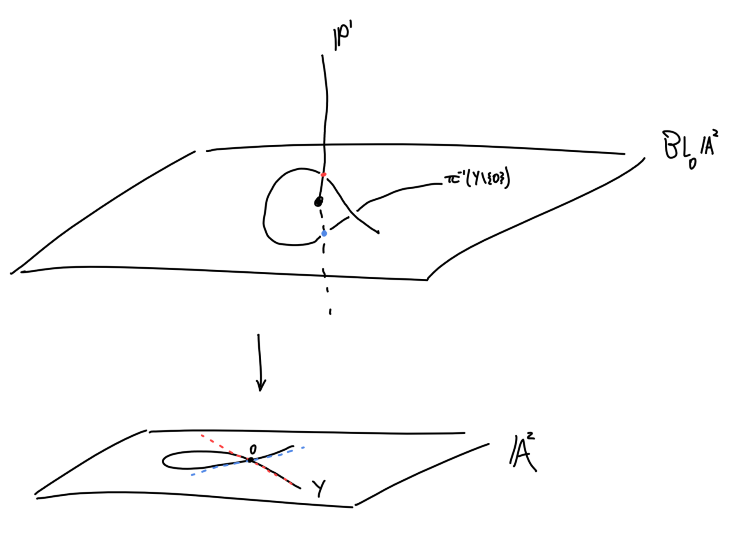
\includegraphics[scale=0.5]{blowup_nodal}
\end{center}

\begin{exercise}
    Consider the cone $Y=V(x^2+y^2-z^2)\subseteq\A^3$, and the point
    $0\hookrightarrow Y$. This is a singular point of $Y$, so we blow it up.
    Show that if $W=V(X^2+Y^2+Z^2)\subseteq\P^2$ then $\Bl_0Y=\O_W(-1)$ is the
    tautological line bundle on $W$.
\end{exercise}

\begin{proof}[Solution]
    We have
    \begin{equation*}
        \pi^{-1}(Y\setminus\{0\})
        = \left\{\bigl((x,y,z),[X:Y:Z]\bigr)
            :xY=yX,xZ=zX,yZ=zY,x^2+y^2=z^2,(x,y,z)\ne(0,0,0)\right\},
    \end{equation*}
    and since $(x,y,z)\ne(0,0,0)$ these equations imply $[X:Y:Z]=[x:y:z]$ and
    hence $X^2+Y^2=Z^2$. On the other hand
    \begin{equation*}
        \O_W(-1) = \left\{\bigl([X:Y:Z],(x,y,z)\bigr)
            :X^2+Y^2+Z^2=0,xY=yX,xZ=zX,yZ=zY\right\},
    \end{equation*}
    so we see that
    $\pi^{-1}(Y\setminus\{0\})=\O_W(-1)\setminus\{\text{zero section}\}$. Hence
    $\Bl_0Y=\closure{\O_W(-1)\setminus\{\text{zero section}\}}=\O_W(-1)$, since
    the complement of the zero section is dense.
\end{proof}

\subsection*{Representation theoretic example}

Consider the ``nilpotent cone''
\begin{equation*}
    \calN_{\SL_2} = \left\{\begin{pmatrix}
            a & b \\ c & -a
    \end{pmatrix}:a^2+bc=0\right\} \subseteq\A^3.
\end{equation*}
The blowup $\Bl_0(\calN_{\SL_2})\xrightarrow\pi\calN_{\SL_2}$ is given by the
cotangent bundle
\begin{equation*}
    T^*(\P^1) = \{(l,\varphi):\text{$l\in\P^1$, $\varphi\in\Hom(\C^2/l,l)$}\};
\end{equation*}
we get from $(l,\varphi)$ to an element of $\calN_{\SL_2}$ by the following
square:
\begin{equation*}
    \begin{tikzcd}
        &V \ar[d,two heads] \ar[r,dashed,"\in\calN_{\SL_2}"] &V \\
        &V/l \ar[r,"\varphi"] &l. \ar[u,hook]
    \end{tikzcd}
\end{equation*}
This is the first instance of the ``Springer resolution''. For a group
$G=\GL_n,\SO_n,\Sp_{2n},\ldots$ we get for the Lie algebra $\g$ a ``nilpotent
cone'' $\calN_{\g}$ and a map
\begin{equation*}
    \calN_\g \leftarrow T^*(G/B)
\end{equation*}
where $B$ is a Borel subgroup, and then $G/B$ is some flag variety like $\P^1$.

\subsection*{What are blow-ups good for?}

\paragraph{1. Resolution of singularities (Hironaka)} Principle: any singular
variety becomes non-singular after finitely many blow-ups:
\begin{equation*}
    \text{non-singular: $\Bl_{Z_n}Y_n$} \to \cdots
        \to \Bl_{Z_1}Y_1 \to Y_1 = \Bl_{Z_0}Y_0 \to Y_0 = Y.
\end{equation*}

\begin{exercise}[Must do]
    Take $V(f)\subseteq\A^2$, where $f(x,y)=x^3-y^2$ with a singularity at
    $(0,0)$. Blow up the singular point $(0,0)$ until you get a smooth curve.
    Now do the same for $f(x,y)=x^{24}-y^{17}$.
\end{exercise}

\begin{proof}[Solution]
    Taking coordinates $(x,y,[X:Y])\in\A^2\times\P^1$ we have
    \begin{align*}
        \Bl_{(0,0)}V(f) \cap \{X\ne0\}
            &= \closure{\left\{(x,y,[1:t]):y^2=x^3,y=xt,(x,y)\ne(0,0)\right\}} \\
            &= \closure{\left\{(x,y,[1:t]):x=t^2,y=xt,t\ne0\right\}} \\
            &= \left\{(x,y,[1:t]):x=t^2,y=xt\right\} \cong \A^1_t,
    \end{align*}
    while
    \begin{align*}
        \Bl_{(0,0)}V(f) \cap \{Y\ne0\}
            &= \closure{\left\{(x,y,[s:1]):y^2=x^3,x=ys,(x,y)\ne(0,0)\right\}} \\
            &= \closure{\left\{(x,y,[s:1]):ys^3=1,x=ys\right\}} \\
            &= \left\{(x,y,[s:1]):ys^3=1,x=ys\right\}
    \end{align*}
    has no points with $s=0$, so this is the whole blow up;
    $\Bl_{(0,0)}V(f)\cong\A^1_t$ via $t\mapsto(t^2,t^3)$. Now $\A^1$ is smooth,
    so we are done.
\end{proof}

\paragraph{2. Birational geometry} Two varieties $Y_1,Y_2$ are
\emph{birational}, which we write $Y_1\sim Y_2$, if there are
non-empty open sets $U_1\subseteq Y_1$, $U_2\subseteq Y_2$ which are isomorphic,
i.e. $U_1\cong U_2$. We say $Y$ is \emph{rational} if
$Y\sim\A^N\sim\P^N$ for some $N$.

\begin{example}
    \begin{itemize}
        \item Take the quadric
            \begin{equation*}
                Q = \{[x_0:\cdots:x_4]:x_0x_4+x_1x_3+x_2^2=0\} \subseteq \P^4,
            \end{equation*}
            which has dimension 3. This is rational:
            \begin{equation*}
                Q \supseteq Q\cap\{x_0\ne0\}
                = \{[1:x_1:x_2:x_3:-x_2^2-x_1x_3]\} \cong \A^3.
            \end{equation*}

        \item A smooth curve $\Sigma_g$ of genus $g$ is rational iff $g=0$.

        \item $\Bl_ZY\sim Y$ via the open set $Y\setminus Z$.
    \end{itemize}
\end{example}

\begin{theorem}[Weak Factorization, Abramovich--Karu--Matsuki--Wlodariczyk]
    Two smooth projecdtive varieties $X,Y$ are birational iff there exists a
    chain of roofs
    \begin{equation*}
        \begin{tikzcd}
            & &W_{01} \ar[dl] \ar[dr] & &W_{12} \ar[dl] \ar[dr] &
                &\cdots \ar[dl] \ar[dr] & \\
            &X=X_0 & &X_1 & &X_2 & &X_n=Y
        \end{tikzcd}
    \end{equation*}
    with each map a blow-up along a smooth subvariety.
\end{theorem}

\begin{exercise}
    Find such a chain (one roof) from the quadric $Q$ above to $\P^3$. (Hint:
    blow up a point in $Q$.) Now replace the dimension 3 with an arbitrary
    dimension $n$. The special case $n=2$ gives a roof from $\P^1\times\P^1$ to
    $\P^2$.
\end{exercise}

\begin{corollary}
    Birational invariants are the same thing as blow-up invariants.
\end{corollary}

\begin{example}
    For example, the Hodge numbers $h^{p,0}(X)$ are blow-up invariants and hence
    birational invariants.
\end{example}

\subsection*{Algebraic definition}

We will know look at two perspectives on a proper definition of the blow-up:
\begin{itemize}
    \item Algebra: ``What else can it be?''
    \item Equations in affine charts: ``How can I compute in practice?''
\end{itemize}

For the first, suppose the embedding $Z\hookrightarrow Y$ is locally given by
$\Spec A/I\to\Spec A$. We want a map $\Bl_ZY\to Y$, which should be projective,
so given by
\begin{equation*}
    \Proj(R) = \Bl_ZY \to Y = \Spec A
\end{equation*}
for some graded $A$-algebra $R$ constructed ``naturally'' from $I$. We have a
summand of $A$ in $R$, and we add a summand of $I$, which forces by products a
summand of $I^2$, and so on, giving the \emph{Rees algebra}:
\begin{equation*}
    R = A\oplus I\oplus I^2\oplus I^3\oplus\cdots = \Sym^\bullet(I);
\end{equation*}
the product is defined via $I^p\cdot I^q\hookrightarrow I^{p+q}$. We may then
define
\begin{equation*}
    \Bl_ZY = \Proj(R) = \Proj(\bigoplus_{m\ge0}I^m) = \Proj(\Sym^\bullet(I)),
\end{equation*}
and check that $\Bl_ZY|_Z=\P(N_{Z/Y})$.

To get equations in affine charts, choose finitely many generators
$I=(f_1,\ldots,f_k)$. These give a surjection
\begin{equation*}
    A^{\oplus k}\twoheadrightarrow I,
\end{equation*}
and applying the functors $\Sym^\bullet$ and $\Proj$ we get a closed embedding
\begin{equation*}
    \Proj(\Sym^\bullet(I)) \hookrightarrow \Proj(\Sym^\bullet(A^{\oplus k}))
        = \P^{k-1}_A = Y\times\P^{k-1}.
\end{equation*}
This restricts to an embedding
\begin{equation*}
    \Bl_ZY
        \hookrightarrow (Y\times\P^{k-1})^\inc
        = \left\{\bigl(y,[T_1:\cdots:T_k]\bigr)\in Y\times\P^{k-1}
                :\rank\begin{pmatrix}
                    T_1 & \cdots & T_k \\ f_1(y) & \cdots & f_k(y)
                \end{pmatrix}<2\right\}.
\end{equation*}
What is this in affine charts? We have
\begin{equation*}
    \Bl_ZY \cap \{T_1\ne0\}
        = \Spec\biggl(A[t_2,\ldots,t_k]
            /(f_2-f_1t_2,\ldots,f_k-f_1t_k)
            /(\text{$f_1$-torsion})\biggr),
\end{equation*}
where $f_i=f_1t_i$ is the incidence relation, and $f_1$-torsion refers to the
values annhilated by powers of $f_1$, which give the extra equations cutting out
$\Bl_ZY$. (Note that the ideal $I=(f_1,\ldots,f_k)$ is made to be principal,
generated by $f_1$, in this chart.)

\begin{example}
    If $Y=\{(x,y):y^2=x\}$ and $I=(x,y)$, we get
    $\Bl_0Y\subseteq(Y\times\P^1)^\inc$ with coordinates
    $\bigl((x,y),[U:V]\bigr)$ satisfying $y^2=x^3$, and the incidence relation
    $xV=yU$. In the chart $U\ne0$ we have variables $x,y,t=V/U$ with relations
    $y-tx$, $t^2x^2-x^3=x^2(t^2-x)$, and the $x^2$ factor is dropped when we mod
    out by $x$-torsion, giving
    \begin{equation*}
        \Bl_0Y\cap\{U\ne0\} = \{(x,y,t):y=tx,x=t^2\} \cong \A^1_t.
    \end{equation*}
    In fact this is the whole blow-up; the point where $U=0$ is not in $\Bl_0Y$.
    (This can be checked in the other chart, or by observing that the curve has
    no vertical tangent.) This blow-up hence gives us the normalization map
    $\A^1_t\to Y$, $t\mapsto(t^2,t^3)$.
\end{example}

\begin{example}
    Blowing up $\P^2$ at 9 (generic) points: Consider generic homogeneous cubics
    $F,G$ in $x,y,z$, with vanishing locus $V(F,G)=\{\text{9 points}\}$. We
    claim the following description of the blow-up:
    \begin{equation*}
        \begin{tikzcd}
            &\bigl([x:y:z],[a:b]\bigr)\ni\P^2\times\P^1 \ar[d]
            &V(aF+bG)=\Bl_{V(F,G)}\P^9 \ar[l,hook] \\
            &\P^2.
        \end{tikzcd}
    \end{equation*}
    Over points with $F=G=0$ the fibre is the whole copy of $\P^1$, and away
    from them $(F,G)\ne(0,0)$ implies $[a:b]$ is uniquely determined by
    $aF+bG=0$.
\end{example}

\newpage

\section{Topology of Manifolds - Simon Donaldson}

We will look at:
\begin{itemize}
    \item Some examples.
    \item Some main ideas.
    \item The reason for the distinction between high and low dimensions that
        appears when classifying manifold topology.
\end{itemize}

\subsection*{Examples and Ideas}

\subsubsection*{The Classification of Surfaces}

Given $n$-dimensional manifolds $M_1,M_2$, we have the connected sum $M_1\#M_2$.
\begin{center}
    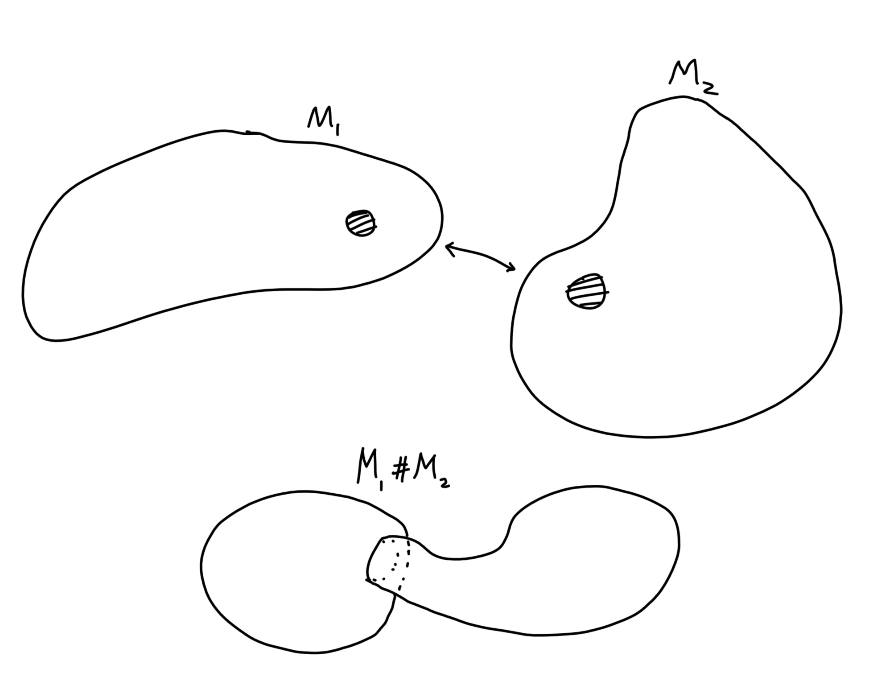
\includegraphics[scale=0.3]{manifolds_connectedsum}
\end{center}
Using this we have the classification of closed surfaces:
\begin{itemize}
    \item Orientable case (no M\"obius bands): $S^2,T^2,T^2\#T^2,\ldots$
    \item Non-orientable case: $\RP^2,\RP^2\#\RP^2,\RP^2\#\RP^2\#\RP^2,\ldots$
\end{itemize}
For $n\ge4$, we can construct a manifold whose fundamental group is given by any
desired finite presentation. Hence we cannot hope for such a classification of
manifolds in these dimensions, since there isn't even an algorithm to decide if
a finite presentation describes the trivial group.

\subsubsection*{Algebraic Topological Data}

Suppose $M^n$ is oriented, smooth and closed. We have many algebraic topological
invariants even when restricting to simply connected manifolds:
\begin{itemize}
    \item $H^*(M;\Z)\xleftrightarrow{\PD}H_*(M;\Z)$ with the cup product /
        intersection product.

    \item We have characteristic classes: the Steifel--Whitney classes $w_i$,
        the Pontryagin classes $p_i(M)=p_i(TM)\in H^{4i}(M;\Z)$. (Defined by
        $p_i(V)=(-1)^ic_{2i}(V\otimes\C)$ where $c_{2i}$ is the Chern class.)

    \item ...
\end{itemize}
If $n=2m$, we get an intersection form $H_m(M)\times H_m(M)\to\Z$ which is
symmetric if $m$ is even and skew-symmetric if $m$ is odd. When $m$ is even this
symmetric form has a signature $\sigma(M)$. For closed manifolds it is
non-degenerate.
\begin{center}
    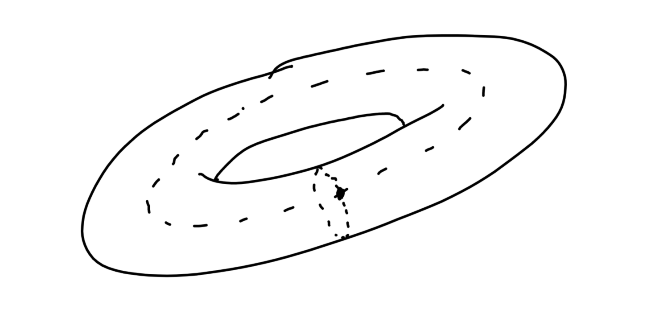
\includegraphics[scale=0.3]{manifolds_intersection}
\end{center}
The classification of such forms over $\Z$ in the skew-symmetric case is simple:
they are sums of blocks of the form
\begin{equation*}
    \begin{pmatrix}
        0 & 1 \\ -1 & 0
    \end{pmatrix}.
\end{equation*}
In the symmetric case the classification over $\R$ is given by the signature,
but over $\Z$ there is a rich theory.

\subsubsection*{Projective Planes}

Beyond the spheres, the simplest homology one can ask for occurs in dimension
$4k$ with $H^0(M)=H^{2k}(M)=H^{4k}(M)=\Z$ and $H^i(M)=0$ otherwise. For $k=1$ we
have the example $\CP^2$, given by attaching $D^4$ to $S^2$ using the Hopf map
$\partial D^4=S^3\to S^2$. Similarly, for $k=2$ we have the projective plane
over the quaternions $\HP^2$, constructed fom a map $S^7\to S^4$. For $k=4$ we
have the Cayley projective plane over the Octonions / Cayley numbers,
constructed from a map $S^{15}\to S^8$. There are no more examples, by some deep
algebraic topology (non-existence of maps with Hopf invariant 1).

\subsubsection*{Plumbing}

Suppose $\Gamma$ is a graph, with numbers $c_i\in\Z$ for each vertex $v_i$. We
construct from this a 4-manifold $X_{\Gamma,\vec c}$ with boundary:
\begin{itemize}
    \item For a vertex $v_i$, take a copy $\Sigma_i$ of $S^2$, and a line bundle
        $L_i\to\Sigma_i$ with $c_1(L_i)=c_i$. (For example if $c_i=-2$ then
        $L_i=T^*\Sigma_i$.) Then let $N_i$ be a tubular neighbourhood of the
        zero section in $L_i$, which is a 4-manifold with boundary.

    \item For an edge between $v_i$ and $v_j$, we glue $N_i$ and $N_j$ as
        follows, with $\Sigma_i$, $\Sigma_j$ transverse:
        \begin{center}
            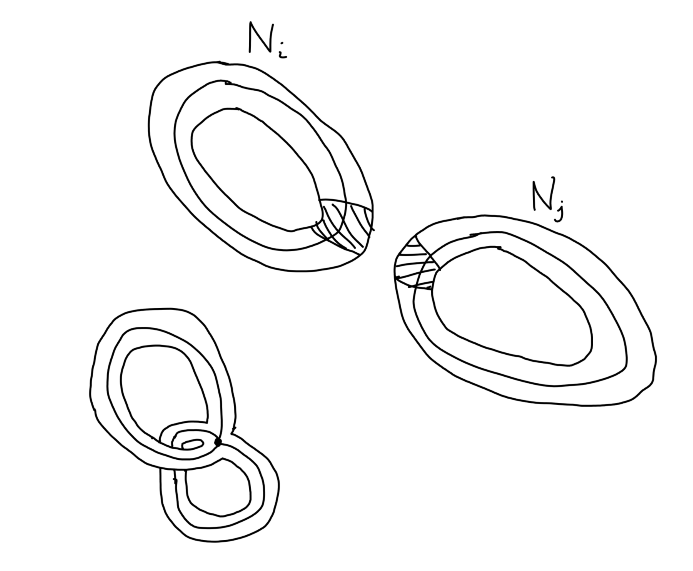
\includegraphics[scale=0.4]{manifolds_plumbing}
        \end{center}
\end{itemize}
Then the intersection form has $c_i$'s for the diagonal entries
(self-intersections) and the adjacency matrix of $\Gamma$ off the diagonal.

\subsubsection*{ADE Manifolds}

Take $c_i=-2$, and let $\Gamma$ be the Dynkin diagram of one of the ADE Lie
algebras.
\begin{itemize}
    \item $A_k$: \dynkin{A}{4}, \ldots
    \item $D_k$: \dynkin{D}{5}, \ldots
    \item The exceptional Lie algebras $E_6,E_7,E_8$, e.g. $E_8$: \dynkin{E}{8}
\end{itemize}
These correspond to finite subgroups of $SU(2)$:
\begin{itemize}
    \item $A_k$: cyclic of order $k+1$
    \item $D_k$: dihedral of order $2k$
    \item $E_6$: tetrahedron, $E_7$: octahedron, $E_8$: icosahedron.
\end{itemize}
Note that we have the double cover $\SU(2)=S^3\to\SO(3)$, so these correspond
roughly to finite subgroups in $\SO(3)$. Moreover we obtain the boundary
$\partial X_\Gamma$ as the quotient $S^3/G$ for the corresponding group $G$.
This gives the 3-manifolds whose universal cover is $S^3$.

\begin{example}
    The simplest case is $A_1$, where there is just one vertex. Then $X_\Gamma$
    is a tubular neighbourhood of $S^2$ in $T^*S^2$, and $\partial X_\Gamma$ is
    $S^3/\{\pm1\}=\RP^3=SO(3)$.
\end{example}

\begin{example}
    In the case $E_8$, the group $G$ is perfect and $\partial X_\Gamma$ is a 
    homology sphere, which was discovered by Poincar\'e. If we add a cone on
    $\partial X_\Gamma$ to $X_\Gamma$ we get a simply connected 4-dimensional
    space $Z$ which is not a manifold but is a ``homology manifold''. The
    intersection form of $Z$ is the $E_8$ quadratic form. Now Rohlin's Theorem,
    from the 1950's, asserts that a simply-connected smooth closed 4-manifold
    with ``even'' intersection form has signature divisible by 16. The $E_8$
    is even with signature -8, so there is no simply-connected smooth closed
    4-manifold with this intersection form.
\end{example}

\subsubsection*{The Pontryagin Classes and Examples in Dimensions 7 and 8}

Let $V\to S^4$ be a rank 4 oriented vector bundle, with structure group $\SO(4)$
after picking a metric. The unit ball bundle gives a manifold $X^8$ with
boundary $\partial X=Y^7$ the unit sphere bundle in $V$.

Now such bundles $V$ are classified by elements of $\pi_3(\SO(4))$ by the
clutching construction, and $\pi_3(\SO(4))=\pi_3(S^3\times S^3)=\Z\oplus\Z$, so
$V$ is given by a pair of integers $(n_+,n_-)\in\Z\oplus\Z$. (Here we use the
double cover $S^3\times S^3=SU(2)\times SU(2)\to\SO(4)$.) The self-intersection
number $d$ of $S^4$ in $X$ is $d=n_+-n_-$, and the Pontryagin class $p_1(X)$
evaluated on $S^4$ is $q=2(n_++n_-)$, so we also recover $V$ from the numbers
$d$ and $q$. From the Serre spectral sequence, one computes that
$H^4(Y)=\Z/d\Z$.
\begin{itemize}
    \item $d=0$: $H^3(Y)=H^4(Y)=\Z$, so $Y$ looks like $S^3\times S^4$ in
        homology, but the non-trivial bundles are distinguished by the different
        values of $q=2(n_++n_-)$.

    \item $d=1$: $H^3(Y)=H^4(Y)=0$, so $Y$ is a homotopy sphere. Then $Y$ is
        homeomorphic to $S^7$ by the generalized Poincar\'e conjecture, but by
        changing $q=2(n_++n_-)$ it turns out one obtains non-diffeomorphic
        manifolds, called \emph{exotic spheres}. (This is due to Milnor.) Adding
        a cone on $Y$ to $X$ then gives a topological 8-manifold with no smooth
        structure.
\end{itemize}

\subsection*{Cobordism, Surgery and the Whitney Trick}

\subsubsection*{Cobordism}

\begin{definition}
    \emph{Oriented cobordism} is an equivalence relation on closed oriented
    $n$-manifolds. Manifolds $M_0^n,M_1^n$ are \emph{cobordant}, written
    $M_0\sim M_1$, if there is an oriented $(n+1)$-manifold $W$ with
    \begin{equation*}
        \partial W = \overline{M_0}\sqcup M_1,
    \end{equation*}
    where $\overline{M_0}$ denotes $M_0$ with reversed orientation. The
    cobordism equivalence classes form an abelian group with the operation of
    disjoint union, written $\Omega_n$.
    \begin{center}
        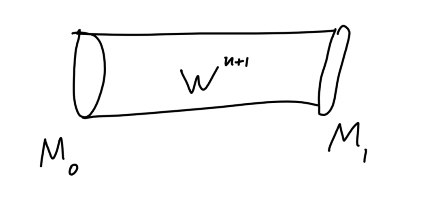
\includegraphics[scale=0.4]{manifolds_cobordism}
    \end{center}
\end{definition}

In dimension $4k$ (other dimensions only have finite cobordism groups), we have
the following cobordism invariants:
\begin{itemize}
    \item The signature $\sigma$.
    \item The \emph{Pontryagin numbers}, which are defined by evaluating certain
        polynomials in the Pontryagin classes on the fundamental class
        $[M]\in H_{4k}(M)$. When $k=1$ we just have the Pontryagin number
        $p_1=\langle p_1,[M]\rangle$. For $k=2$ we have
        \begin{equation*}
            p_1^2 = \langle p_1(M)^2,[M]\rangle \quad \text{and} \quad
            p_2 = \langle p_2(M),[M]\rangle,
        \end{equation*}
        for $k=3$ we have $p_1^3,p_1p_2,p_3$, and so on.
\end{itemize}

\begin{theorem}[The Hirzebruch Signature Theorem]
    The signature $\sigma(M)$ can be expressed as a rational polynomial in the
    Pontryagin numbers.
\end{theorem}

\begin{remark}
    The fact that the coefficients are rational while the signature is an
    integer has important consequences, in a similar vein to Rohlin's Theorem.
\end{remark}

\begin{example}
    In dimensions 4 and 8 we have $\sigma(M^4)=p_1/3$ and
    $\sigma(M^8)=(7/45)p_2-(1/45)p_1^2$. In general the Bernoulli numbers are
    involved in the coefficients.
\end{example}

\subsubsection*{Surgery}

In fact any cobordism is a composite of particular elementary cobordisms called
``surgeries''.

\begin{definition}
    If $\Sigma\subseteq M^n$ is an embedded $p$-sphere with given trivialization
    of its normal bundle, we define the \emph{surgery along $\Sigma$} as
    follows. The trivialization gives a tubular neighbourhood
    $N\cong S^p\times B^{n-p}$, with
    \begin{equation*}
        \partial N
            \cong S^p\times S^{n-p-1}
            \cong \partial(B^{p+1}\times S^{n-p-1}).
    \end{equation*}
    We then remove $N$, and glue $N'=B^{p+1}\times S^{n-p-1}$ in its place along
    $\partial N\cong\partial N'$, obtaining a new manifold $M'$ which is the
    result of surgery.
\end{definition}

\begin{example}
    When $p=0$ we get the self-connected sum. The connected sum is hence surgery
    on the disjoint union.
\end{example}

\begin{remark}
    There is a standard cobordism from $M$ to $M'$ given by attaching a
    ``handle'' to $M\times[0,1]$. The handle $H=B^{p+1}\times B^{n-p}$ is an
    $(n+1)$-dimensional $(p+1)$-handle, with
    \begin{equation*}
        \partial H
            = (S^p\times B^{n-p})\cup(B^{p+1}\times S^{n-p-1})
            = N\cup N',
    \end{equation*}
    with the intersection of $N$ and $N'$ in $\partial H$ given by
    $\partial N\cong\partial N'$. Hence we can glue $H$ to $M\times\{1\}$ along
    $N$, which results in applying the above surgery to $M\times\{1\}$ in the
    boundary of $M\times[0,1]$. This is called an \emph{elementary cobordism}.
    (Note that technically we need to smooth the corners in this gluing in order
    to preserve the smooth structure. This can be done in a standard way.)
    \begin{center}
        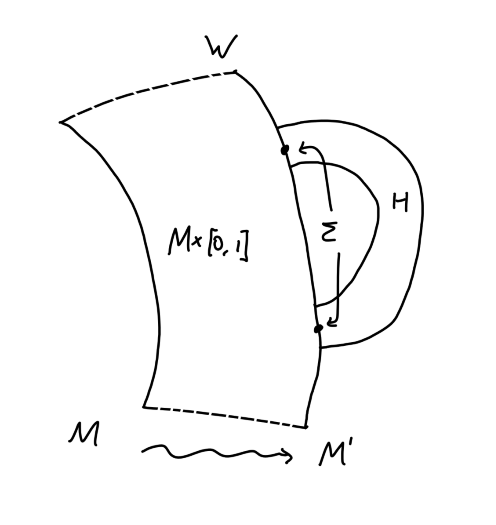
\includegraphics[scale=0.5]{manifolds_surgery}
    \end{center}
\end{remark}

\subsubsection*{Morse Theory}

A fundamental motivation for the notion of cobordism comes from considering
families of equations. For example, suppose that $F:X\to T$ is a smooth map, and
for $t\in T$ let $Z_t\subseteq X$ be the set of solutions to the equation
$F(x)=t$. For generic $t$ the solution set $Z_t$ is a manifold of dimension
$n=\dim(X)-\dim(T)$. For different generic values $t_0,t_1$ the manifolds
$Z_{t_0}$, $Z_{t_1}$ may not be diffeomorphic, but are cobordant. To see this,
join $t_0,t_1$ by a path $\gamma:[0,1]\to T$ and let $W\subseteq X\times[0,1]$
be the set
\begin{equation*}
    W = \{(x,s):F(x)=\gamma(s)\}.
\end{equation*}
For a generic path $\gamma$ this will be a manifold of dimension $n+1$ giving a
cobordism from $Z_{t_0}$ to $Z_{t_1}$. A similar discussion applies to other
families of equations, such as zero sets of sections of vector bundles. The
ideas can also be extended to certain infinite dimensional situations, for
example moduli spaces of holomorphic curves.

\begin{example}
    Consider hypersurfaces $X\subseteq\RP^5$ defined by homogeneous polynomials
    of degree 4. The polynomial $x_0^4-(x_1^4+x_2^4+x_3^4+x_4^4)$ gives a
    4-sphere. For different polynomials we get many other 4-manifolds, but we
    can never get $\CP^2$ since it is not cobordant to 0.
\end{example}

To generate cobordisms by elementary cobordisms, we look at the special values
of $t\in T$ where $Z_t$ changes diffeomorphism type; where it fails to be a
manifold.

\begin{example}
    Take $\R^{n+1}$ with coordinates $x_1,\ldots,x_q,y_1,\ldots,y_{p+1}$ where
    $p+q=n$. Let $f:\R^{n+1}\to\R$ be the quadratic form $|x|^2-|y|^2$. Then
    $f^{-1}(-1)$ contains a sphere $\Sigma=S^p$, and $f^{-1}(1)$ contains a
    sphere $S^{q-1}$. The manifold $f^{-1}(1)$ is obtained from $f^{-1}(-1)$ by
    surgery along $\Sigma$, and $f^{-1}[-1,1]$ is diffeomorphic to the standard
    elementary cobordism realizing this surgery.
    \begin{center}
        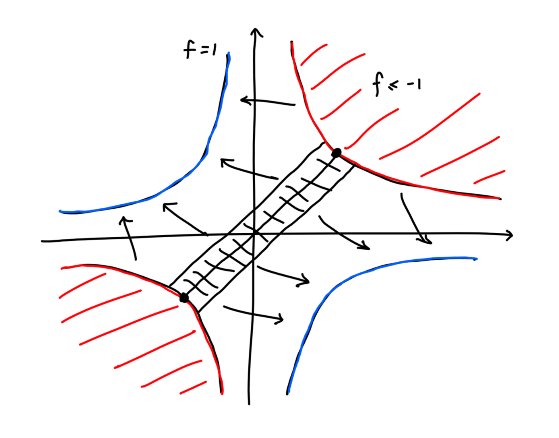
\includegraphics[scale=0.5]{manifolds_morse1}
    \end{center}
\end{example}

In general, for a cobordism $W$ from $M_0$ to $M_1$ we consider a particularly
nice type of function $f:W\to[0,1]$ known as a \emph{Morse function}, with
$f^{-1}(1)=M_1$, $f^{-1}(0)=M_0$. There are finitely many critical values of $f$
in $[0,1]$, and the manifolds $M_t=f^{-1}(t)$ change by a surgery as $t$ crosses
each critical value, giving a factorization of $W$ into elementary cobordisms.
The number $p+1$ in the surgery is the \emph{index} of the critical point, which
can be read off from the Hessian of $f$. (In fact in a neighbourhood of a
critical point, the Morse function can be written in the form $|x|^2-|y|^2$ as
in the previous example using suitable coordinates.)
\begin{center}
    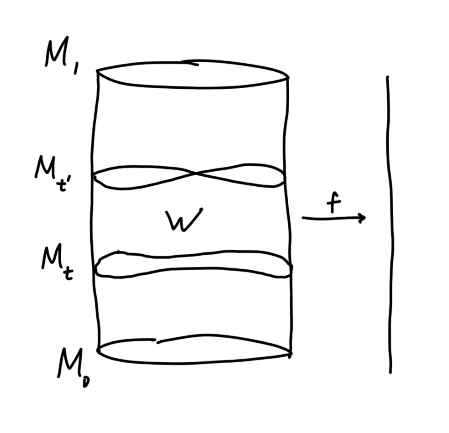
\includegraphics[scale=0.4]{manifolds_morse2}
\end{center}

\begin{example}
    Let $K\subseteq S^3$ be an embedded circle, i.e. a knot. The boundary of a
    tubular neighbourhood $N$ of $K$ is a torus $T$. There is a well-defined
    meridian $\mu\in H_1(T)$ which bounds a disc in $N$. To specify surgery we
    need a class $\gamma\in H_1(T)$ with $\gamma\cdot\mu=1$, which will then
    bound a disc in the solid torus $N'$ which we attach. There is a unique
    longitudinal class $\lambda\in H_1(T)$ with $\lambda\cdot\mu=1$ such that
    $\lambda$ maps to 0 in $H_1(S^3\setminus N)$, so we can take
    $\gamma=\lambda+c\mu$ for any integer \emph{surgery coefficient} $c$. Now
    let $L\subseteq S^3$ be a link with components $K_i$. Perform surgery on
    each component with coefficients $c_i$ to get a 3-manifold $Y$ which is the
    boundary of a 4-manifold $X$. Then $H_2(X)$ has a basis $\{\sigma_i\}$ in 
    which the intersection form has diagonal entries the $c_i$'s and
    off-diagonal entries the linking numbers $\lk(K_i,K_j)$. The cobordism group
    $\Omega_3$ vanishes, which implies that all closed 3-manifolds are obtained
    by this construction. We get another description of the ADE manifolds
    $X_\Gamma$ by taking a link with unknotted components whose linking matrix
    corresponds to the graph $\Gamma$ with coefficients $-2$.
\end{example}

\subsubsection*{The Whitney Trick}

Suppose $M^n$ is simply-connected, and $P^p$, $Q^q$ are transverse
path-connected submanifolds of $M$, with $p+q=n$. They then have finitely many
signed intersection points. Suppose $a,b\in P\cap Q$ have opposite sign. Can we
``cancel'' them? The Whitney trick says: yes, if $p,q\ge3$. (In fact this can be
made sharper, by following carefully the actual requirements of the proof.)
Specifically, we can find $P'$ isotopic to $P$ with
$P'\cap Q=(P\cap Q)\setminus\{a,b\}$. For example, if the algebraic intersection
$P\cdot Q=0$ then we can isotope $P$ to be disjoint from $Q$.

\begin{proof}[Sketch of proof]
    By path-connectedness, we have paths from $a$ to $b$ in $P$ and $Q$, giving
    a loop $\gamma$ in $P\cup Q$. As $M$ is simply-connected we have a
    null-homotopy $D^2\hookrightarrow M$, $\partial D^2=\gamma$, and for
    dimension reasons we can perturb this to an embedding disjoint from $P,Q$
    away from $\gamma$. Since the signs of $a$ and $b$ are opposite, we can
    trivialize the normal bundle of $\gamma$ suitably to get a neighbourhood of
    $D$ in $M$ diffeomorphic to a standard model of the situation in Euclidean
    space:
    \begin{center}
        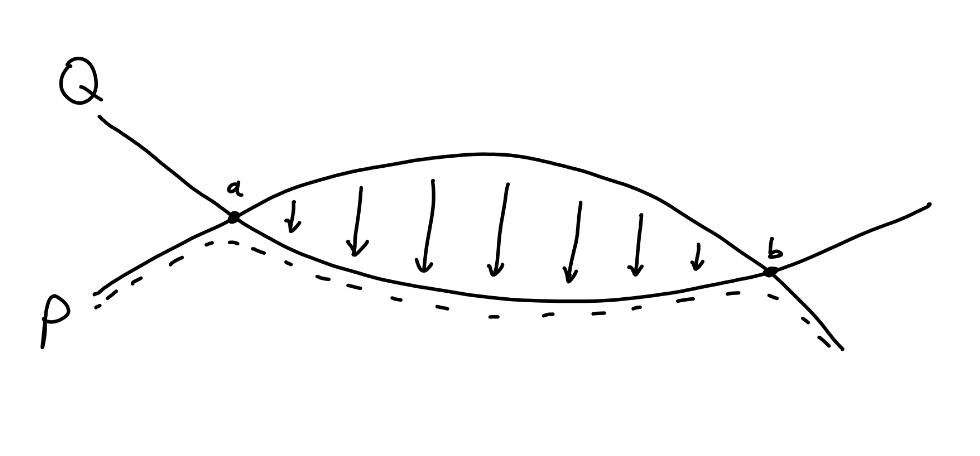
\includegraphics[scale=0.3]{manifolds_whitney}
    \end{center}
    In this model we then write down an explicit isotopy removing the
    intersections as follows, which can be transported along the diffeomorphism
    back to $M$.
\end{proof}

\begin{remark}
    This result is the basic fact that distinguishes high- and low-dimensional
    manifold topology. In dimension 4 with $p=q=2$ the argument fails since the
    disc is no longer generically disjoint from $P$ and $Q$, and no longer
    generically embedded (it may have self-intersection points). The details
    that need checking about frames along $\gamma$ for the trivialization also
    fail. In fact the conclusion is false.
\end{remark}

\begin{remark}
    In dimension 3 there are famous results such as Dehn's Lemma and The Loop
    Theorem in a similar spirit, which are proved in an entirely different way.
\end{remark}

\subsubsection*{The $h$-Cobordism Theorem}

Using the Whitney trick, we obtain the following fundamental result:

\begin{theorem}[The $h$-Cobordism Theorem]
    Suppose $M_0^n,M_1^n$ are simply-connected manifolds of dimension $n\ge5$
    cobordant via a simply-connected cobordism $W^{n+1}$. Suppose that the
    inclusions $M_i\hookrightarrow W$ induce isomorphisms on homology. Then
    $M_0,M_1$ are diffeomorphic and $W\cong M_0\times[0,1]$.
\end{theorem}

\begin{proof}[Sketch of proof]
    Choose a Morse function $f_0$ on $W$ to represent it as a composition of
    surgeries. If $f_0$ has no critical points then we clearly have
    $W\cong M_0\times[0,1]$, so our strategy is to attempt to remove critical
    points from $f_0$. To give the main idea, assume $n=6$ and $f_0$ has two
    critical points $u,v\in W$. The hypothesis on homology implies that $u,v$
    have index difference 1. Assume $u$ has index 3 and $v$ has index 4, with
    levels $f_0(u)=1/4$ and $f_0(v)=3/4$. Write $M=f^{-1}(1/2)$. Crossing these
    critical points exhibit $M_0$ and $M_1$ as the results of surgeries on $M$
    along spheres $P_u,P_v\subseteq M$. The hypothesis on homology implies that
    the intersection number of $P_u$ and $P_v$ is $\pm1$. Using the Whitney
    trick we can then suppose $P_u$ and $P_v$ have a single (transverse)
    intersection point. Then a neighbourhood of $P_u\cup P_v$ in $M$ has a
    standard model and we can write down a deformation of $f_0$ which cancels
    the critical points.
\end{proof}

\begin{remark}
    One important application of the $h$-cobordism theorem is the generalized
    Poincar\'e conjecture for higher dimensions: If $n\ge5$ and $M^n$ is
    homotopy equivalent to $S^n$, then $M^n$ is homeomorphic to $S^n$. It also
    leads to classification results for higher-dimensional manifolds with
    topological restrictions, e.g. any 2-connected 6-manifold is diffeomorphic
    to a connected sum of copies of $S^3\times S^2$.
\end{remark}

\subsection*{Exercises}

\begin{enumerate}
    \item Let $F_r$ be the free group on $r$ generators and $\gamma\in F_r$. For
        $n\ge4$ use surgery on a connected sum of $r$ copies of
        $S^1\times S^{n-1}$ to construct an $n$-dimensional manifold with
        fundamental group $F_r/\langle\gamma\rangle$. Why does this not work if
        $n=3$?
        \begin{proof}[Solution]
            If $M_0$ is the connected sum of $r$ copies of $S^1\times S^{n-1}$,
            then $\pi_1(M_0)=\overbrace{\Z*\cdots*\Z}^{\text{$r$ times}}=F_r$ by
            the Seifert-Van Kampen theorem; the intersections contract onto
            $S^{n-1}$, which is simply-connected. (This requires $n\ge3$.)
            Representing $\gamma$ by a loop in $M_0$, we perform surgery along
            $\gamma$ to get a manifold $M$. Writing $N(\gamma)$ for a tubular
            neighbourhood of $\gamma$, the Seifert-Van Kampen theorem gives
            \begin{align*}
                \pi_1(M)
                    = \pi_1(M_0\setminus N(\gamma))
                        *_{\pi_1(\partial N(\gamma))}\pi_1(B^2\times S^{n-2})
                    = \pi_1(M_0\setminus N(\gamma))*_{\langle\gamma\rangle}1,
            \end{align*}
            noting that $\pi_1(S^{n-2})=1$ since $n\ge4$. We also have
            \begin{align*}
                \pi_1(M_0)
                    = \pi_1(M_0\setminus N(\gamma))
                        *_{\pi_1(\partial N(\gamma))}\pi_1(N(\gamma)),
            \end{align*}
            and the map $\pi_1(\partial N(\gamma))\to\pi_1(N(\gamma))$ is an
            isomorphism as $S^{n-2}\to B^{n-2}$ induces the trivial map on
            trivial groups, so $\pi_1(M_0\setminus N(\gamma))=\pi_1(M_0)$. Hence
            \begin{equation*}
                \pi_1(M)
                    = \pi_1(M_0)/\langle\gamma\rangle
                    = F_r/\langle\gamma\rangle.
            \end{equation*}
        \end{proof}

    \item Show that $\RP^2\#\RP^2\#\RP^2$ and $T^2\#\RP^2$ are homeomorphic.

        Let $\overline{\CP^2}$ denote $\CP^2$ with reversed orientation. Show
        that no two of
        \begin{equation*}
            S^2\times S^2,\,\CP^2\#\CP^2,\,\CP^2\#\overline{\CP^2}
        \end{equation*}
        are homeomorphic, but $(S^2\times S^2)\#\overline{\CP^2}$ is
        homeomorphic to $\CP^2\#\overline{\CP^2}\#\overline{\CP^2}$.

        (Complex geometry may be helpful here. Blowing up a point on a complex
        surface corresponds to connected sum with $\overline{\CP^2}$.)

        \begin{proof}[Solution]
            The fact $\RP^2\#\RP^2\#\RP^2\cong T^2\#\RP^2$ is a classic part of
            the classification of surfaces, which I won't reproduce here. For
            the 4-manifolds
            $S^2\times S^2,\CP^2\#\CP^2,\CP^2\#\overline{\CP^2}$, note that they
            all have Betti numbers $1,0,2,0,1$. So homology groups aren't enough
            to distinguish them, so we look at the ring structure on cohomology
            instead, i.e. the intersection form.
            \begin{itemize}
                \item For $S^2\times S^2$, generators for $H^2$ are given by
                    $S^2\times\{*\}$ and $\{*\}\times S^2$, which intersect
                    transversely and with positive orientation at the single
                    point $(*,*)$. The self-intersections are zero, since
                    $S^2\times\{*\}$ is disjoint from $S^2\times\{*'\}$, so the
                    intersection form is given by
                    \begin{equation*}
                        Q_{S^2\times S^2} = \begin{pmatrix}
                            0 & 1 \\ 1 & 0
                        \end{pmatrix}.
                    \end{equation*}

                \item For $\CP^2\#\CP^2$, the generators for $H^2$ are given by
                    lines $\CP^1$ in each copy of $\CP^2$. The self-intersection
                    of a line in $\CP^2$ is 1, and we can take a line in one
                    copy not meeting the other copy, so the intersection form is
                    given by
                    \begin{equation*}
                        Q_{\CP^2\#\CP^2} = \begin{pmatrix}
                            1 & 0 \\ 0 & 1
                        \end{pmatrix}.
                    \end{equation*}

                \item For $\CP^2\#\overline{\CP^2}$, we have almost exactly the
                    same story as for $\CP^2\#\CP^2$, except the
                    self-intersection of a line in $\overline{\CP^2}$ is $-1$,
                    so the intersection form is given by
                    \begin{equation*}
                        Q_{\CP^2\#\overline{\CP^2}} = \begin{pmatrix}
                            1 & 0 \\ 0 & -1
                        \end{pmatrix}.
                    \end{equation*}
            \end{itemize}
            Now these matrices are not congruent; $Q_{\CP^2\#\CP^2}$ is
            positive-definite, while the others are indefinite, and
            $Q_{S^2\times S^2}$ is even, while $Q_{\CP^2\#\overline{\CP^2}}$ is
            odd. Hence we see that the manifolds are not homeomorphic.

            However, note that $(S^2\times S^2)\#\overline{\CP^2}
            =(\CP^1\times\CP^1)\#\overline{\CP^2}$ is the blow-up of
            $\CP^1\times\CP^1$ at a point, while
            $\CP^2\#\overline{\CP^2}\#\overline{\CP^2}$ is the blow-up of
            $\CP^2$ at two points. From what we saw in the section on blowing
            up these are isomorphic complex varieties, and therefore
            homeomorphic manifolds.
        \end{proof}

    \item Let $X$ be the 4-manifold corresponding to the $A_2$ graph
        \dynkin{A}{2}. Show that $\pi_1(\partial X)=\Z/3$.

        \begin{proof}[Solution]
            Recall that $\partial X$ was the quotient of $\SU(2)\cong S^3$ by
            the finite subgroup corresponding to the Dynkin diagram in question.
            For $A_2$ this is the cyclic rotation group of the $(2+1)$-gon, i.e.
            $C_3$. Hence $\pi_1(\partial X)=\pi_1(S^3/C_3)=\Z/3$.
        \end{proof}

    \item Let $W$ be an oriented $(2n+1)$-manifold with boundary $M$. There is a
        boundary map
        \begin{equation*}
            \partial:H_{n+1}(W,M)\to H_n(M).
        \end{equation*}
        Use duality and the long exact sequence in cohomology to show that the
        image of $\partial$ is an isotropic subspace in $H_n(M)$ with respect to
        the intersection form (i.e. $\partial a\cdot\partial b=0$ for all $a,b$)
        of dimension $\frac{1}{2}\dim H_n(M)$. In the case when $n$ is even,
        deduce that the signature of $M$ is zero.

        For an oriented surface $\Sigma$ of genus $g$ denote
        $\lambda^i(\Sigma)=\Lambda^{g+i}(H^1(\Sigma))$. Let $\Sigma_0,\Sigma_1$
        be oriented surfaces of genus $g_0,g_1$ respectively and let $W$ be a
        cobordism from $\Sigma_0$ to $\Sigma_1$. Show that $W$ defines, up to an
        overall factor, linear maps
        \begin{equation*}
            \lambda^i_W:\lambda^i(\Sigma_0)\to\lambda^i(\Sigma_1).
        \end{equation*}
        Investigate how your construction behaves with respect to composition of
        cobordisms.

        (Hint: A $p$-dimensional subspace of a vector space $V$ defines an
        element in $\Lambda^p(V)$, up to a factor.)

        \begin{proof}[Solution]
            Looking at Poincar\'e duality on the long exact sequence of the
            pair, we have
            \begin{equation*}
                \begin{tikzcd}
                    &H_{n+1}(W,M;\R) \ar[r,"\partial"]
                    &H_n(M;\R) \ar[r,"i_*"]
                    &H_n(W;\R) \\
                    &H^n(W;\R) \ar[r,"i^*"] \ar[u,"\PD"]
                    &H^n(M;\R) \ar[r,"\delta"] \ar[u,"\PD"]
                    &H^{n+1}(W,M;\R). \ar[u,"\PD"]
                \end{tikzcd}
            \end{equation*}
            Now the universal coefficients theorem implies that $i^*$ is dual to
            $i_*$, so
            \begin{align*}
                \dim H_n(M;\R) - \dim\im\partial
                    &= \dim H_n(M;\R) - \dim\im i^* \quad \text{by vertical PD} \\
                    &= \dim H_n(M;\R) - \dim\im i_* \quad \text{by duality} \\
                    &= \dim\ker i_* \quad \text{by rank-nullity} \\
                    &= \dim\im\partial \quad \text{by exactness.}
            \end{align*}
            Hence $L=\im\partial$ has dimension $\frac{1}{2}\dim H_n(M;\R)$. For
            $\alpha\in H^n(M;\R)$, $\beta\in H^n(W;\R)$, we have
            \begin{equation*}
                \langle\alpha\cup i^*\beta,[M]\rangle
                    = \langle i^*\beta,[M]\cap\alpha\rangle
                    = \langle\beta,i_*([M]\cap\alpha)\rangle.
            \end{equation*}
            Then for any $\gamma\in H^n(W;\R)$ we get
            \begin{equation*}
                \langle i^*\gamma\cup i^*\beta,[M]\rangle
                    = \langle\beta,i_*([M]\cap i^*\gamma)\rangle
                    = \langle\beta,
                        \cancelto{0}{i_*\partial}([W]\cap\gamma)\rangle
                    = 0,
            \end{equation*}
            so $i^*\gamma\cup i^*\beta=0$. Therefore $\im\partial\cong\im i^*$
            are isotropic for the intersection / cup products. Taking a basis
            $v_1,\ldots,v_r$ for $L$, we can find $w_j$ with
            $v_i\cdot w_j=\delta_{ij}$, and moreover $w_j\cdot w_j=0$ after
            adding a suitable multiple of $v_j$. This gives a basis for
            $H_n(M;\R)$ with respect to which the intersection form is a direct
            sum of factors of the form
            \begin{equation*}
                \begin{pmatrix}
                    0 & 1 \\ (-1)^n & 0
                \end{pmatrix}.
            \end{equation*}
            If $n$ is even these factors have signature zero, and hence the
            signature of $M$ is zero.

            For $W$ a cobordism from $\Sigma_0$ to $\Sigma_1$, we then have that
            the kernel $L$ of
            \begin{equation*}
                \R^{2g_0}\oplus\R^{2g_1}
                    = H_1(\Sigma_0;\R)\oplus H_1(\Sigma_1;\R)\to H_1(W;\R)
            \end{equation*}
            has dimension $g_0+g_1$, and is isotropic for the intersection form.
            Now the maximal dimension of an isotropic subspace of
            $H_1(\Sigma)=\R^{2g}$ is $g$, by writing down the intersection form
            explicitly. Therefore $L=L_0\oplus L_1$ for $L_0$ a
            $g_0$-dimensional isotropic subspace of $H_1(\Sigma_0;\R)$ and $L_1$
            a $g_1$-dimensional isotropic subspace of $H_1(\Sigma_1;\R)$.

            ???
        \end{proof}

    \item Show that $\CP^n$ is not a boundary when $n$ is even. Construct
        manifolds $W_m$ with $\partial W_m=\CP^{2m+1}$.

        (Hint: Consider a map from $\CP^{2m+1}$ to quaternionic projective space
        $\HP^m$.)

        \begin{proof}[Solution]
            From 4. we have that the middle Betti number of an even-dimensional
            boundary is even, so since $H_{2m}(\CP^{2m})=\Z$ has rank 1 we see
            that $\CP^{2m}$ cannot be a boundary. Now for $\CP^{2m+1}$ consider
            the fibre bundle
            \begin{equation*}
                \CP^{2m+1}
                    = (\C^{2m+2}\setminus\{0\})/\C^\times
                    = (\H^{m+1}\setminus\{0\})/\C^\times
                    \to (\H^{m+1}\setminus\{0\})/\H^\times
                    = \HP^m.
            \end{equation*}
            The fibres are given by 
            \begin{equation*}
                \H^\times/\C^\times
                = \frac{\left\{\begin{pmatrix}
                    z & w \\ \conj w & \conj z
                \end{pmatrix}:|z|^2+|w|^2\ne0\right\}}{\left\{\begin{pmatrix}
                    z & 0 \\ 0 & \conj z
                \end{pmatrix}:|z|\ne0\right\}}
                = \left\{\begin{pmatrix}
                    1 & z \\ \conj z & 1
                \end{pmatrix}\right\}\cup\left\{\begin{pmatrix}
                    0 & 1 \\ 1 & 0
                \end{pmatrix}\right\} = \C\cup\{\infty\} = S^2,
            \end{equation*}
            and so we can glue 3-balls $B^3$ onto the fibres (using Alexander's
            trick for compatibility) to get a $B^3$ bundle $W_m$ over $\HP^m$
            with boundary the $S^2$ bundle $\CP^{2m+1}$ over $\HP^m$.
        \end{proof}

    \item The Hopf invariant of a smooth map $f:S^{4k-1}\to S^{2k}$ can be
        defined as follows. Choose a $2k$-form $\omega$ on $S^{2k}$ of integral
        1. Then choose a $(2k-1)$-form $\alpha$ on $S^{4k-1}$ such that
        $f^*(\omega)=d\alpha$. The Hopf invariant is
        \begin{equation*}
            H(f) = \int_{S^{4k-1}}\alpha\wedge f^*(\omega).
        \end{equation*}
        Show that this is well-defined, independent of the choices of
        $\omega,\alpha$.

        Let $X$ be a closed manifold of dimension $4k$ which has a decomposition
        $X=B^{4k}\cup N$ where $N$ is a tubular neighbourhood of a $2k$-sphere
        $\Sigma\subseteq X$ with $\Sigma\cdot\Sigma=1$, so $\partial N$ is a
        $(4k-1)$-sphere. If $\Omega$ is a closed $2k$-form on $X$ with integral
        1 over $\Sigma$ show that
        \begin{equation*}
            \int_X\Omega^2=1.
        \end{equation*}
        By constructing a suitable form $\Omega$, show that the Hopf invariant
        of the map $S^{4k-1}=\partial N\to S^{2k}$ is 1.

    \item Let $M$ be the 8-manifold constructed in the first section from a
        vector bundle $V\to S^4$, with $d=n_+-n_-=1$ and $Y=\partial M$. Let $Z$
        be the space obtained by adding a cone over $Y$ to $M$. Suppose that $Y$
        is diffeomorphic to $S^7$ so that $Z$ is a smooth 8-manifold. Use the
        signature theorem to show that $p_2=(1/7)(45+q^2)$ where $q=2(n_++n_-)$.
        Hence derive a contradiction to the assumption that $Y$ is diffeomorphic
        to $S^7$ for certain values of $n_+,n_-$.

    \item Use Alexander duality to show that a knot $K\subseteq S^3$ bounds an
        oriented surface $\Sigma$ embedded in $S^3\setminus K$ (a \emph{Seifert
        surface}). The surface $\Sigma$ is homeomorphic to a closed surface of
        some genus $g$, minus a disc. Now perform surgery on $K$ with
        coefficient $c>0$ to construct a 3-manifold $Y$ which is the boundary of
        a 4-manifold $X$. Show that
        \begin{itemize}
            \item $H^2(X)=\Z$ and a generator is represented by an embedded
                surface in $X$ of genus $g$ and self-intersection $c$.
            \item $H^1(Y)=\Z/c$.
        \end{itemize}
        (For the first part, recall that $H^1(S^3\setminus K)$ can be identified
        with homotopy classes of maps from $S^3\setminus K$ to $S^1$.)
\end{enumerate}

\section{Geometric Invariant Theory - Tom Coates}

GIT is a way of taking quotients in algebraic geometry.

\paragraph{Why?} Examples: $\P^n=(\C^{n+1}\setminus\{0\})/\C^*$, $\Gr(k,N)$,
toric varieties, projective hypersurfaces / complete intersections. Moduli
problems: want to make a choice of coordinates and then remove that choice. For
$\Gr(k,N)$, a $k$-dimensional subspace of $\C^N$ is determined by a matrix of
spanning vectors:
\begin{equation*}
    \overbrace{\begin{pmatrix}
        * & \cdots & * \\
        \vdots & \ddots & \vdots \\
        * & \cdots & *
    \end{pmatrix}}^{k\times N},
\end{equation*}
up to change of basis, which is an action of $\GL(k)$. We want to quotient by
$\GL(k)$ to get $\Gr(k,N)$.

\paragraph{Context.} Symplectic reduction (a way of taking quotients in
symplectic geometry) is often equivalent to the GIT quotient (Kirwan,
Kemp--Ness). Things to look at from here: infinite-dimensional analogues of
symplectic reduction (Atiyah and Bott, moduli of vector bundles; Donaldson,
K\"ahler--Einstein metrics and K-stability), birational geometry via variation
of GIT quotient or VGIT (Thaddeus, Dolgachev--Hu, \ldots), derived categories
and wall crossings (Ed Segal, \ldots).

\paragraph{References.}
\begin{itemize}
    \item Main source: ``Notes on GIT and symplectic reduction'',
        Richard Thomas.
    \item ``Mirror symmetry for toric complete intersections'',
        Alexander Givental.
    \item ``Topology of torus actions on symplectic manifolds'',
        Mich\'ele Audin.
    \item Francis Kirwan's thesis.
\end{itemize}

\subsection*{Varieties}

We recap some of the basic setup for algebraic geometry, working over $\C$.

\paragraph{Affine varieties.} Affine space $\C^n$ is associated to the ring of
polynomial functions on it: $\C[x_1,\ldots,x_n]$. An affine variety is
a locus $X=\{p_1=\cdots=p_k=0\}\subseteq\C^n$ for some
$p_1,\ldots,p_k\in\C[x_1,\ldots,x_n]$. It is associated with the ring of
restricted polynomials $\O_X=\C[x_1,\ldots,x_n]/(p_1,\ldots,p_k)$.
We can reverse the correspondence: given a suitable ring $\O_X$, picking
generators $g_1,\ldots,g_n\in\O_X$ gives
$\C[x_1,\ldots,x_n]\twoheadrightarrow\O_X$, $x_i\mapsto g_i$, corresponding to
$X\hookrightarrow\C^n$ via $(g_1,\ldots,g_n)$.

\paragraph{Projective varieties.} The motto is ``just work
$\C^*$-equivariantly''. A $\C^*$ action on a ring is a grading, so we work with
\emph{graded} polynomial rings (for simplicity we will assume everything is
generated in degree 1). Projective space $\P^n$ corresponds to the graded ring
$\C[x_0,\ldots,x_n]$. A projective variety is a locus $X=\{p_1=\cdots=p_k=0\}$
for some homogeneous (i.e. $\C^*$-equivariant) polynomials
$p_1,\ldots,p_k\in\C[x_0,\ldots,x_n]$. It is associated with the graded ring of
restricted polynomials $\C[x_0,\ldots,x_n]/(p_1,\ldots,p_k)$. By compactness,
the only global functions we get are constants ($\C^*$-invariant = degree 0 =
constant), so $\C[x_0,\ldots,x_n]$ is \emph{not} the ring of functions. What is
it?

We have an associated affine variety
\begin{equation*}
    \tilde X = \{p_1=\cdots=p_k=0\} \subseteq \C^{n+1},
\end{equation*}
which is $\C^*$-equivariant, i.e. it is a cone through the origin.
\begin{center}
    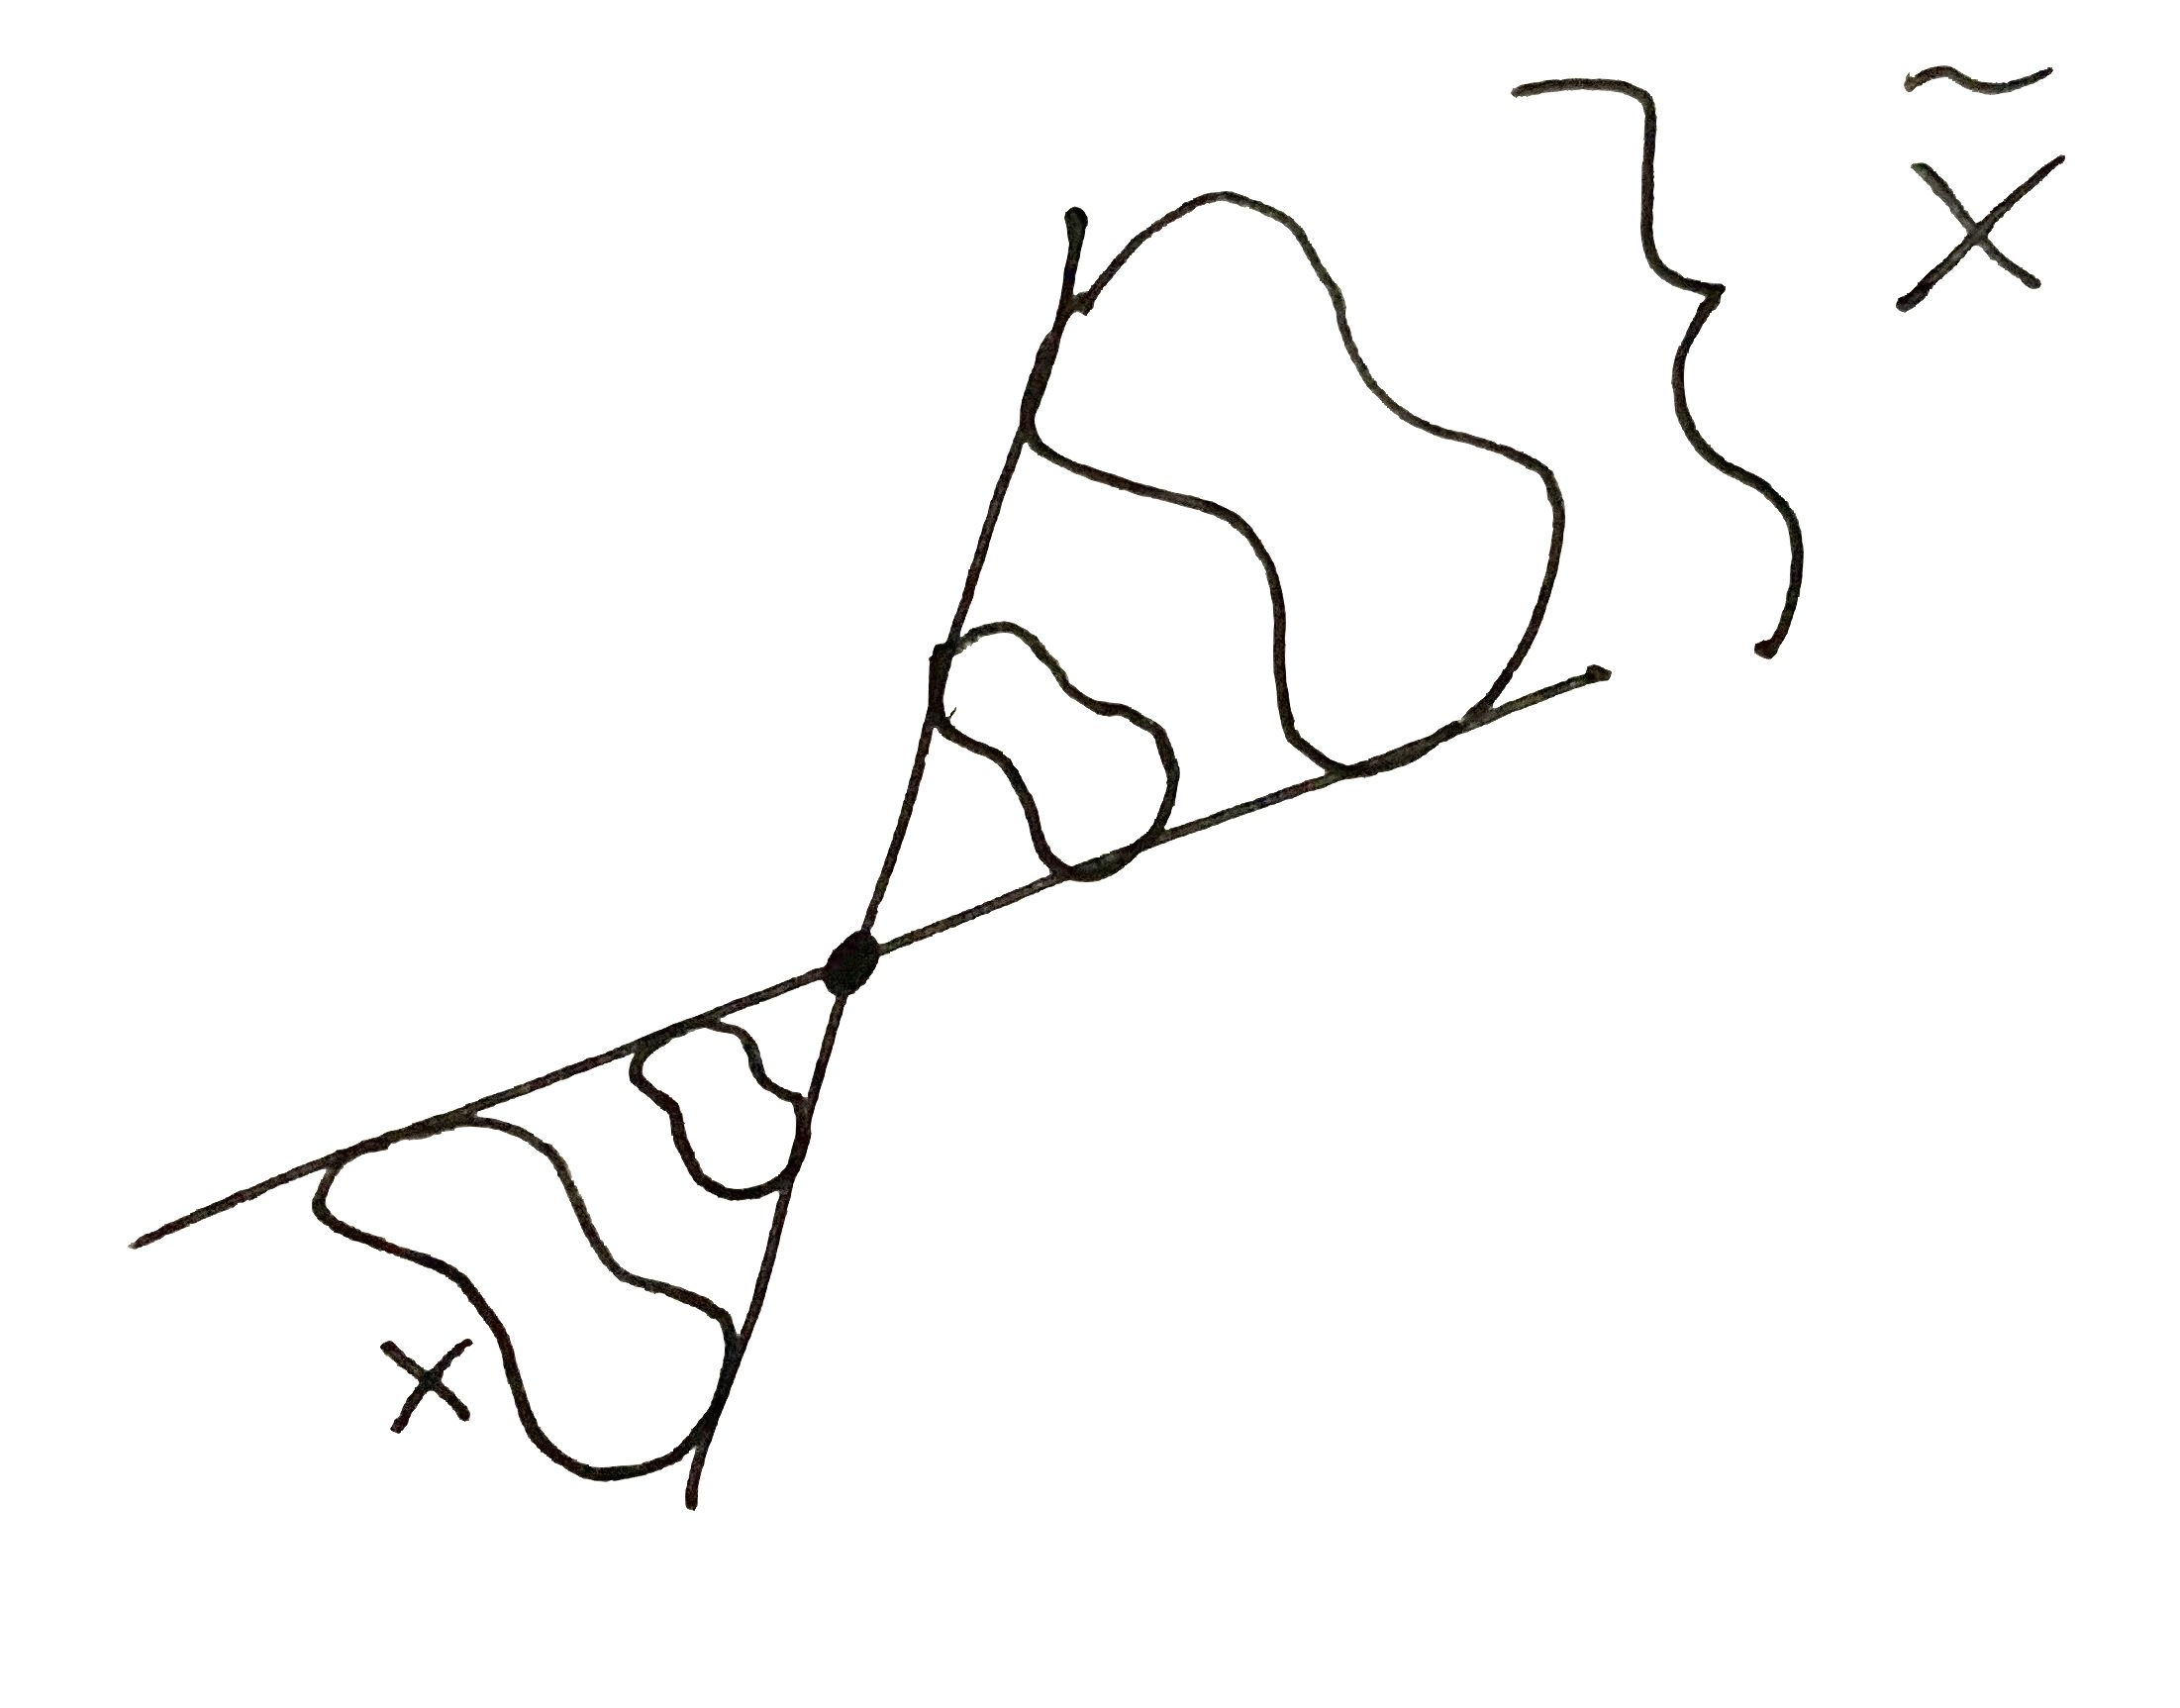
\includegraphics[scale=0.1]{git_cone}
\end{center}

The projective variety $X$ is the parameter space of the lines through the
origin making up $\tilde X$. So we get a tautological line bundle $\O_X(-1)$,
where $\O_X(-1)|_x=\{\text{the line in $\tilde X$ defined by $x$}\}$ for
$x\in X$. The total space of $\O_X(-1)$ naturally maps to $\tilde X$:
\begin{center}
    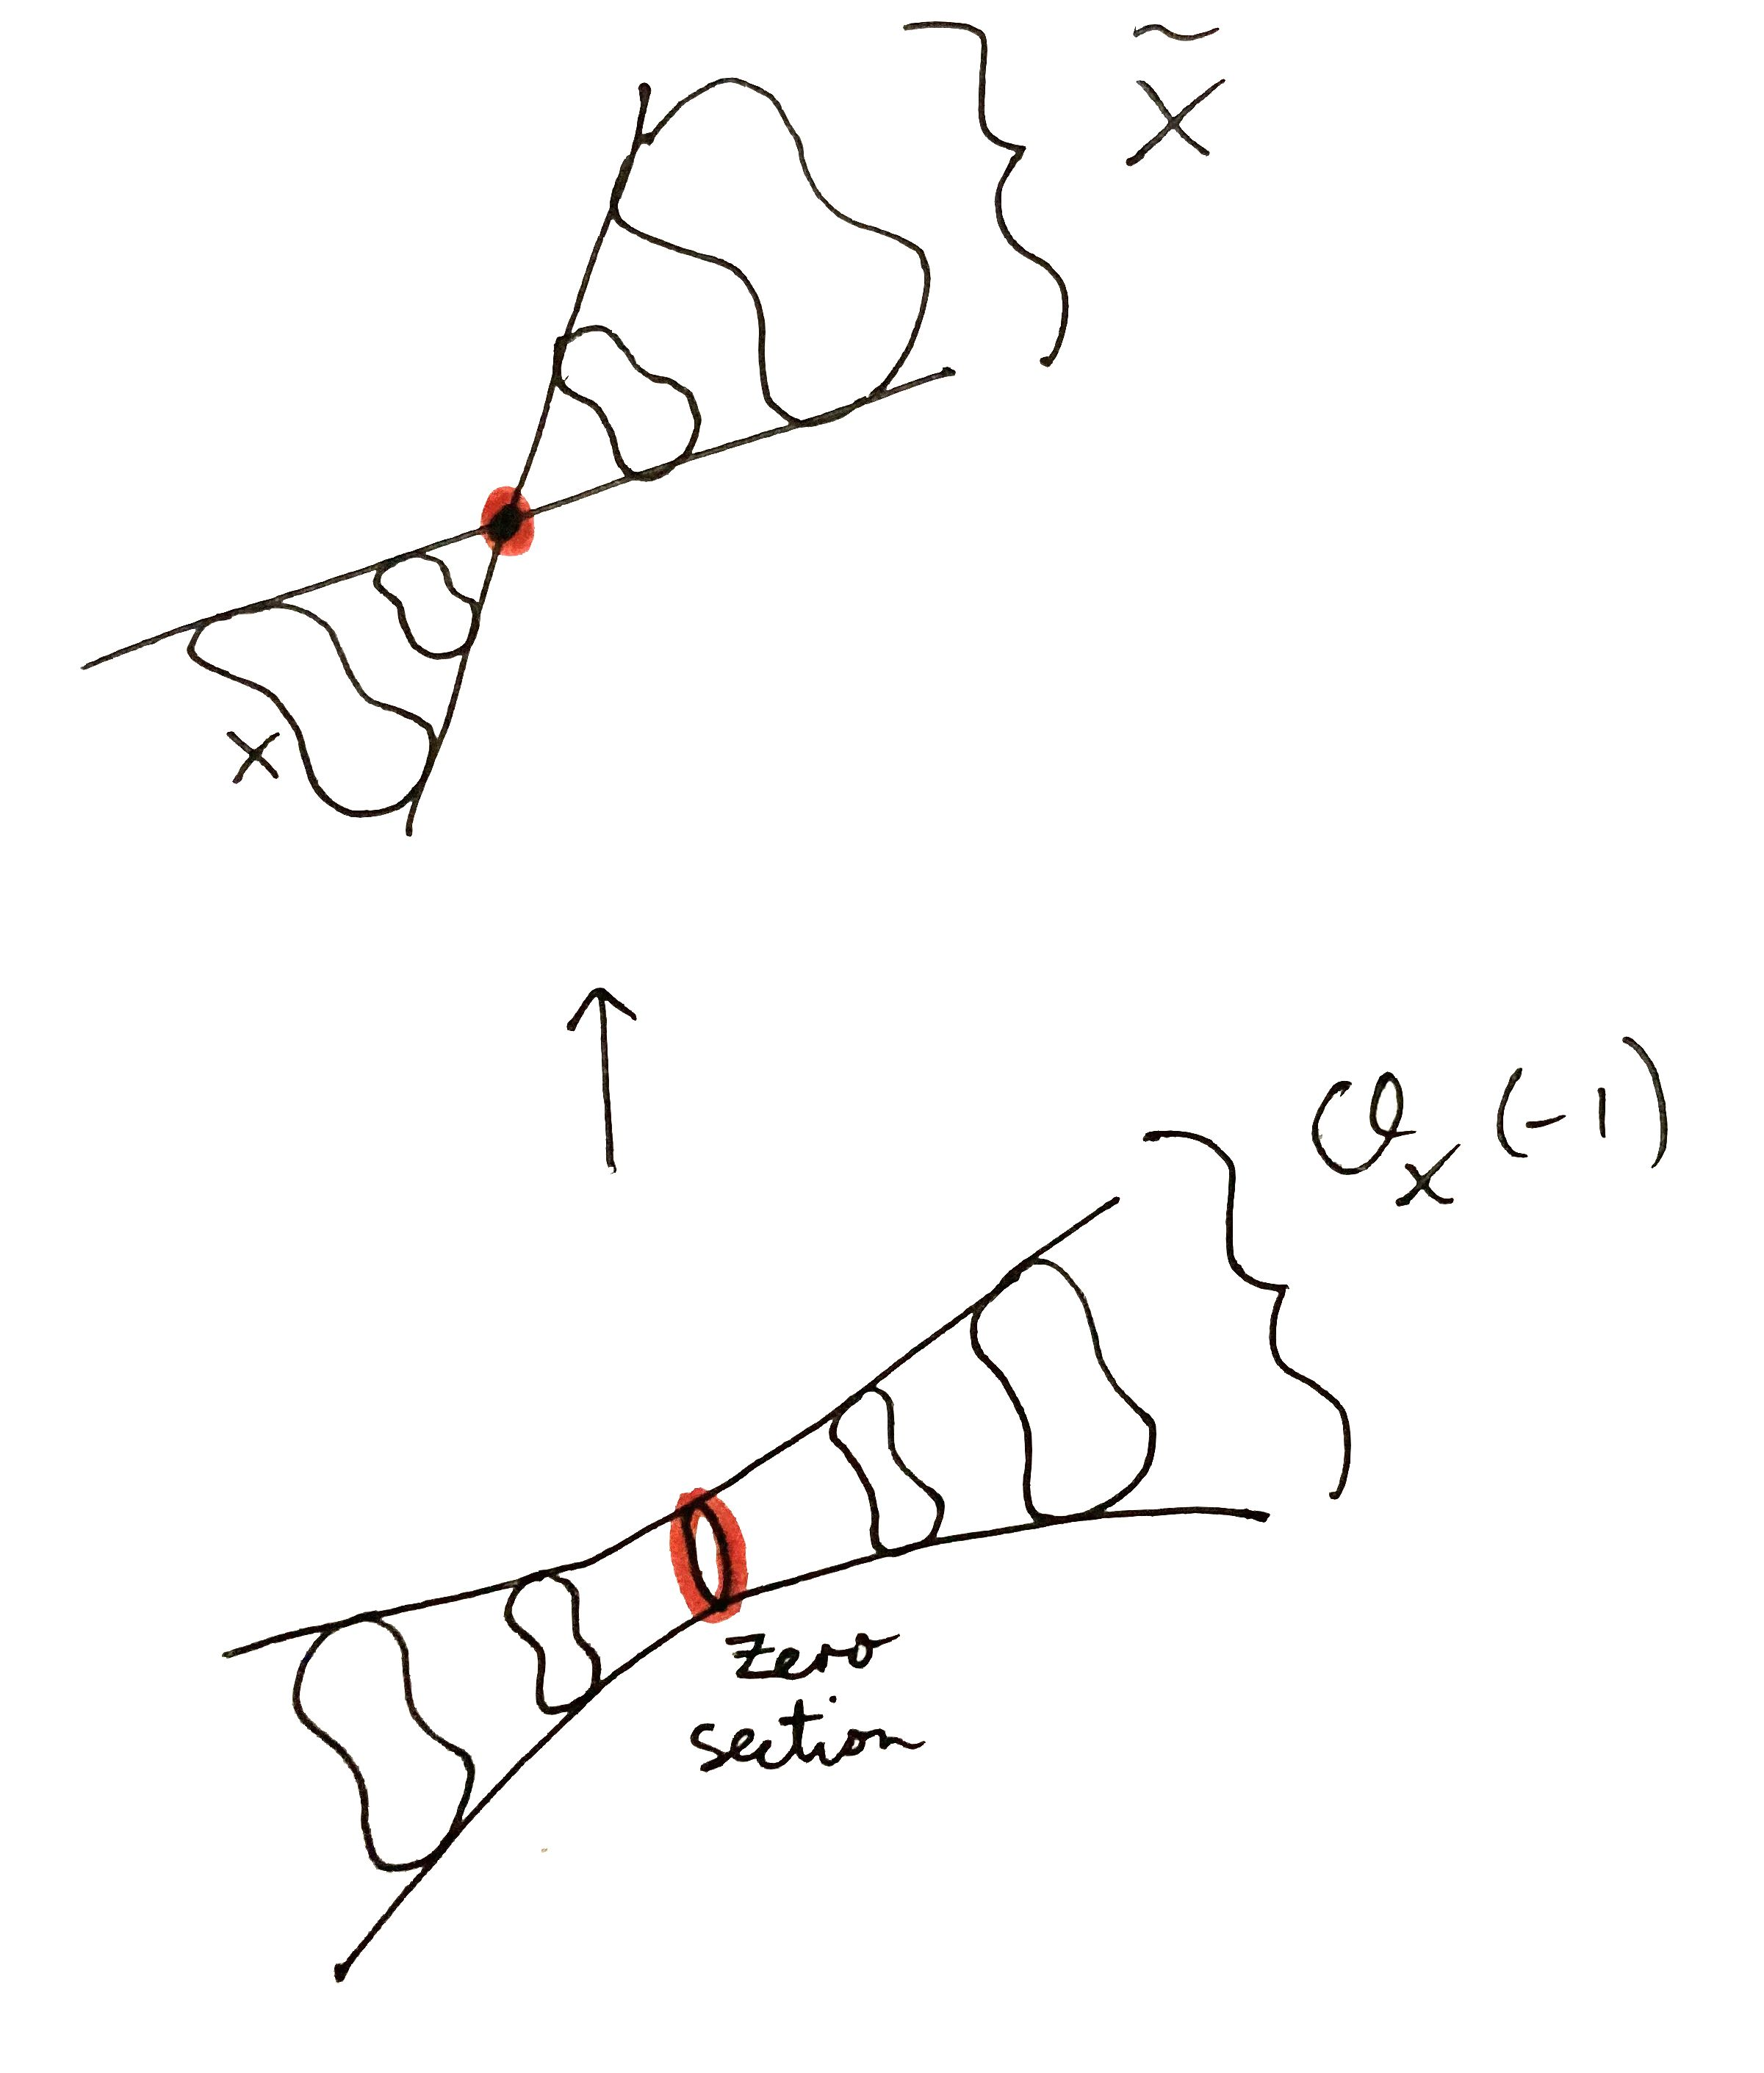
\includegraphics[scale=0.1]{git_blowup}
\end{center}

This is the blowup of the cone vertex!

Each $x_i\in\C[x_0,\ldots,x_n]$ is a linear function on $\C^{n+1}$, so by
pullback we get a function on the total space of $\O_X(-1)$ which is linear on
the fibres. Similarly, a degree $r$ homogeneous polynomial gives a function on
$\O_X(-1)$ which scales with degree $r$ along the fibres. In other words, degree
1 elements of $\C[x_0,\ldots,x_n]$ are sections of $\O_X(-1)^\vee=\O_X(1)$, and
degree $r$ elements are sections of $\Sym^r\O_X(-1)^\vee=\O_X(r)$. Hence
\begin{equation*}
    \C[x_0,\ldots,x_n]/(p_1,\ldots,p_k) = \bigoplus_{k=0}^\infty H^0(\O_X(k)),
\end{equation*}
so we recover the graded ring from the line bundle $\O_X(1)$. (To reverse the
correspondence, choosing generators for $H^0(X,L)$ for a suitable line bundle
$L$ gives an embedding $X\to\P^n$ where $n=\dim H^0(X,L)$.)

\subsection*{Quotients}

Suppose we have a connected reductive complex algebraic group $G$. This means we
have a compact real Lie group $K<G$ such that $G$ is the complexification of
$K$. Examples: $K=S^1$, $G=\C^*$; $K=(S^1)^m$, $G=(\C^*)^m$; $K=\SU(m)$,
$G=\SL(m,\C)$.

Consider an (algebraic) action of $G$ on a projective variety $X$, where we want
to take the quotient ``$X/G$''. Suppose the action can be factored through
$\SL(n+1,\C)$ acting on $\P^n$:
\begin{equation*}
    \begin{tikzcd}
        G \ar[d,hook] & X \ar[loop left, distance=60] \ar[d,hook] \\
        \SL(n+1,\C) & \P^n \ar[loop left, distance=30]
    \end{tikzcd}
\end{equation*}
The choice of this lifting $G\to\SL(n+1,\C)$ is called \emph{linearization}.
(You might ask, why $\SL(n+1,\C)$ rather than just $\Aut(\P^n)=\PSL(n+1,\C)$? It
is because the action of $\PSL(n+1,\C)$ doesn't lift to $\O(-1)$.)

\paragraph{Issues.} The topological quotient is not Hausdorff (essentially
because $X$ is compact but $G$ is non-compact). There are low-dimensional orbits
in the closure of high-dimensional orbits. For example, take the action of
$\C^*$ on $\C^{n+1}$ from the definition of $\P^n$.
\begin{center}
    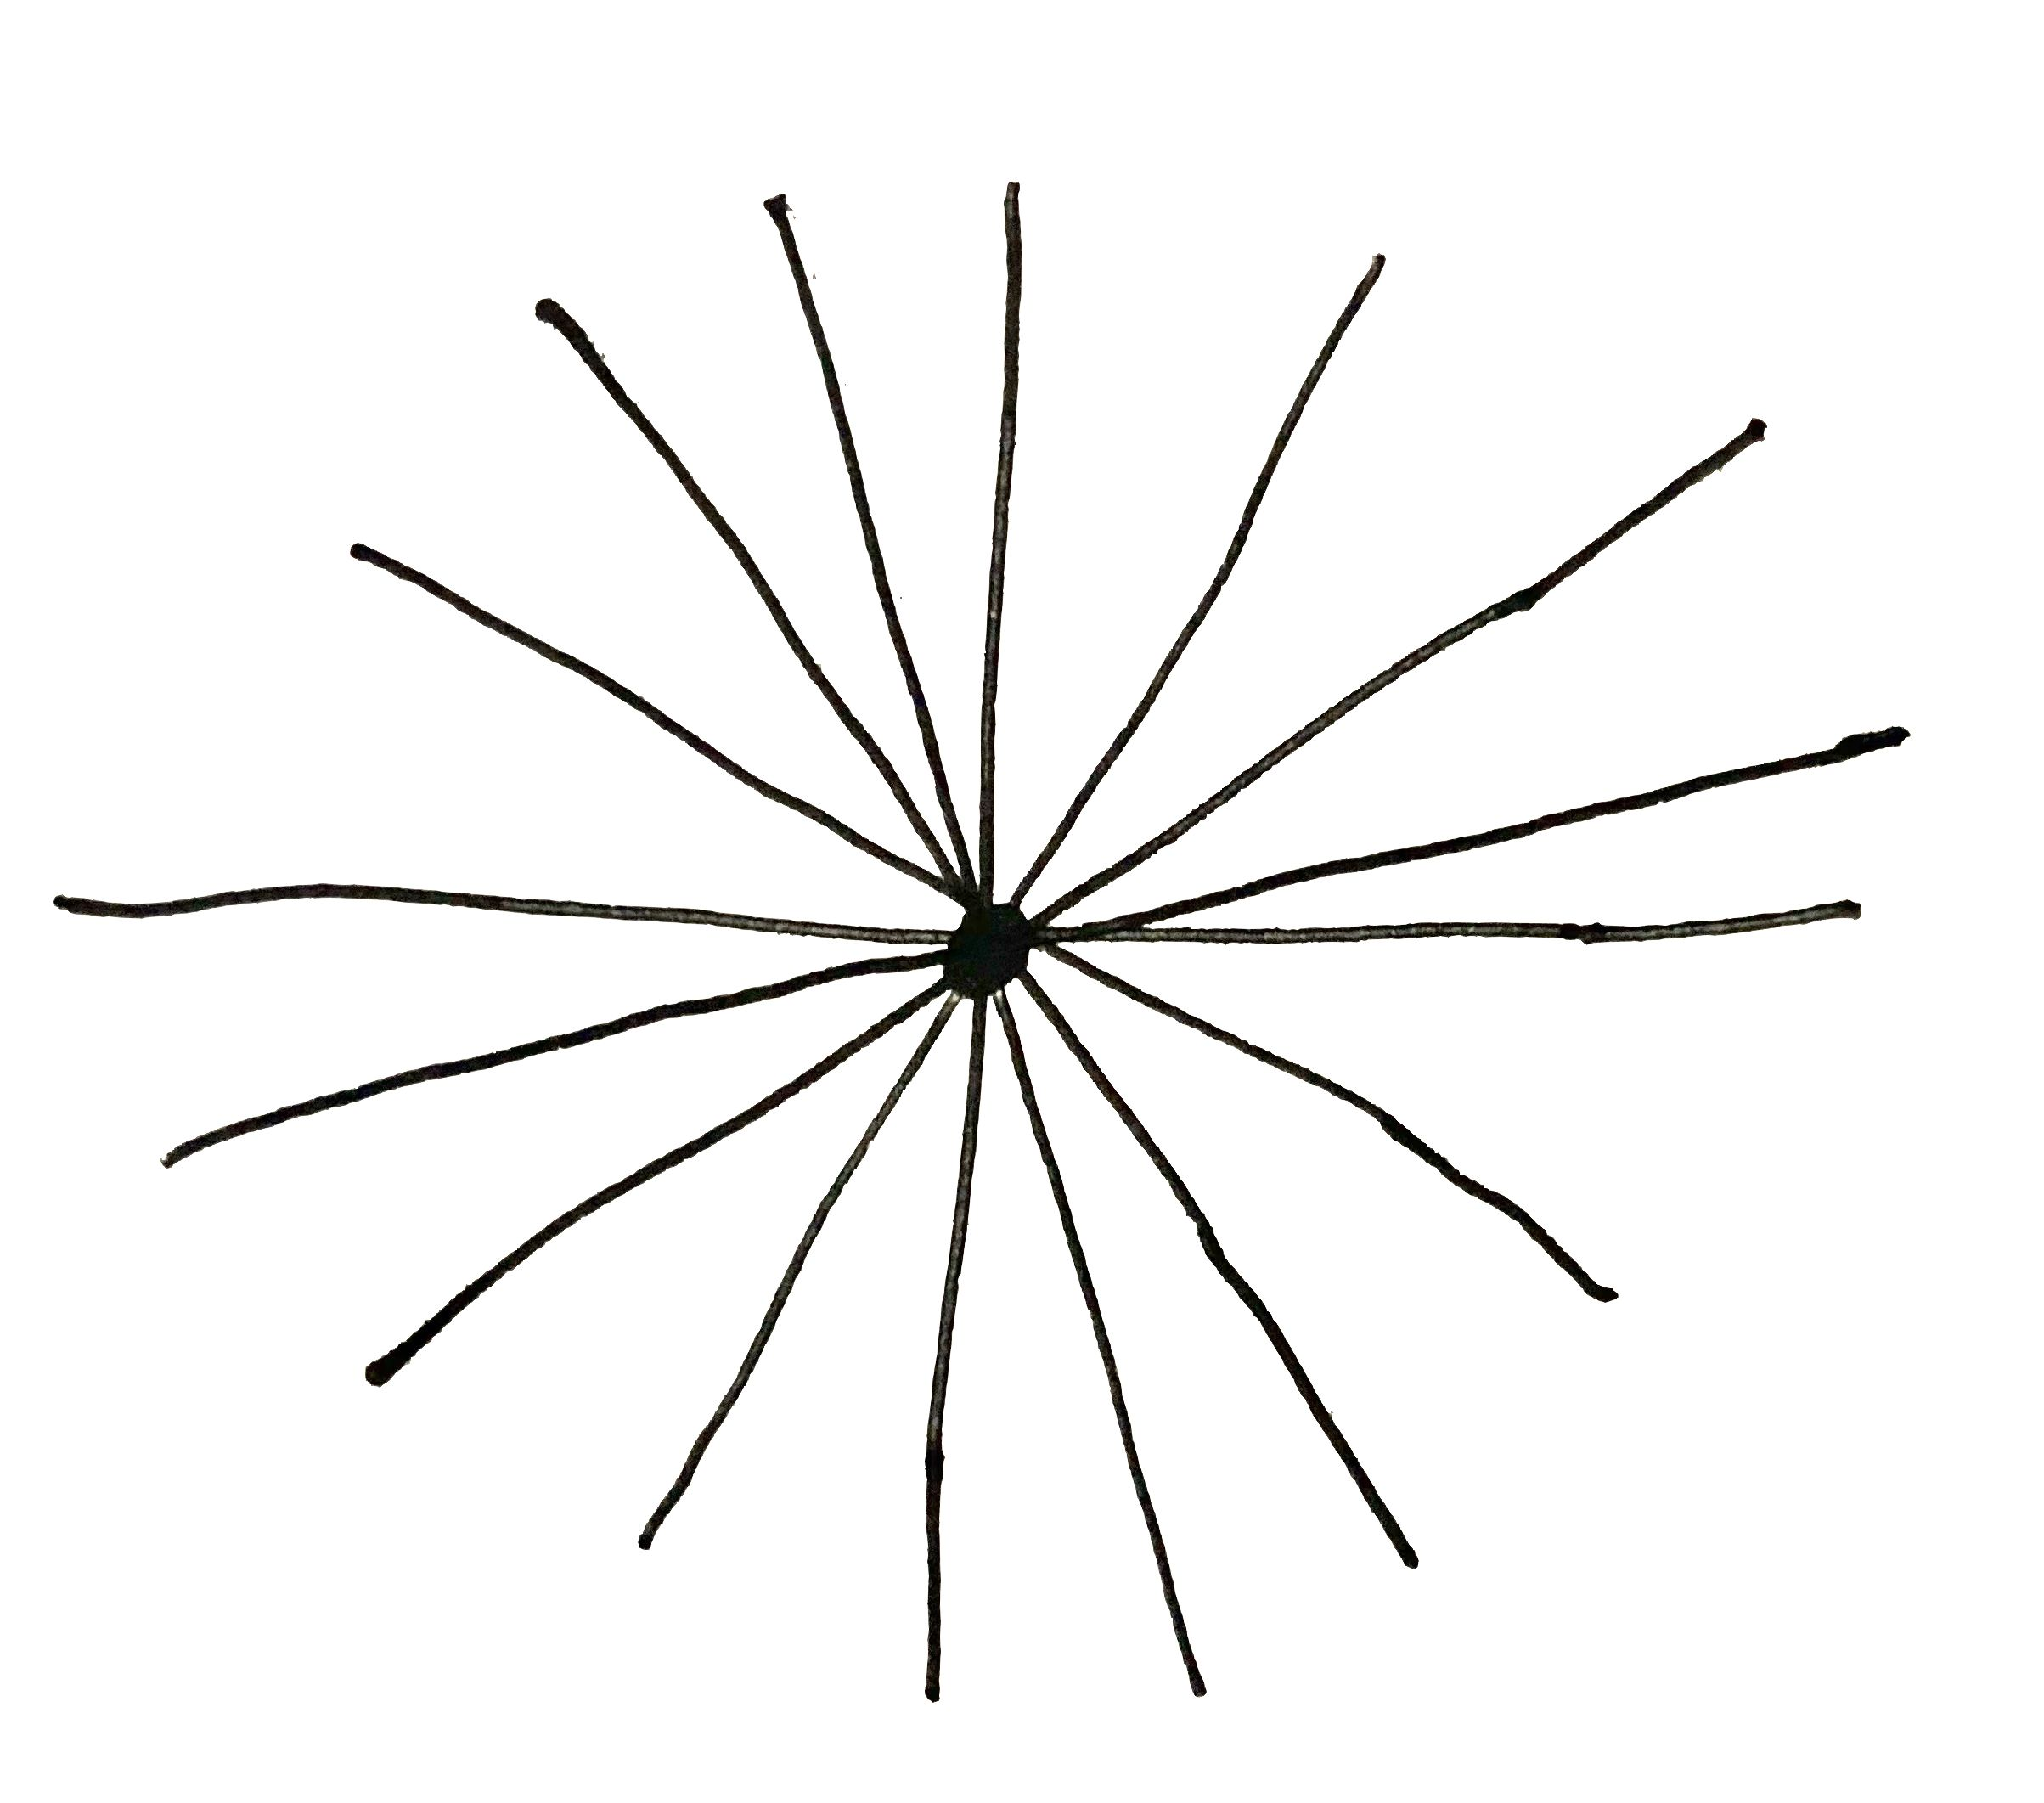
\includegraphics[scale=0.03]{git_node}
\end{center}

The origin is in the closure of every other orbit.

Removing the low-dimensional orbits does not fix the problem. Consider
$\C^*\curvearrowright\C^2$ by $\lambda\cdot(x,y)=(\lambda x,\lambda^{-1}y)$:
\begin{center}
    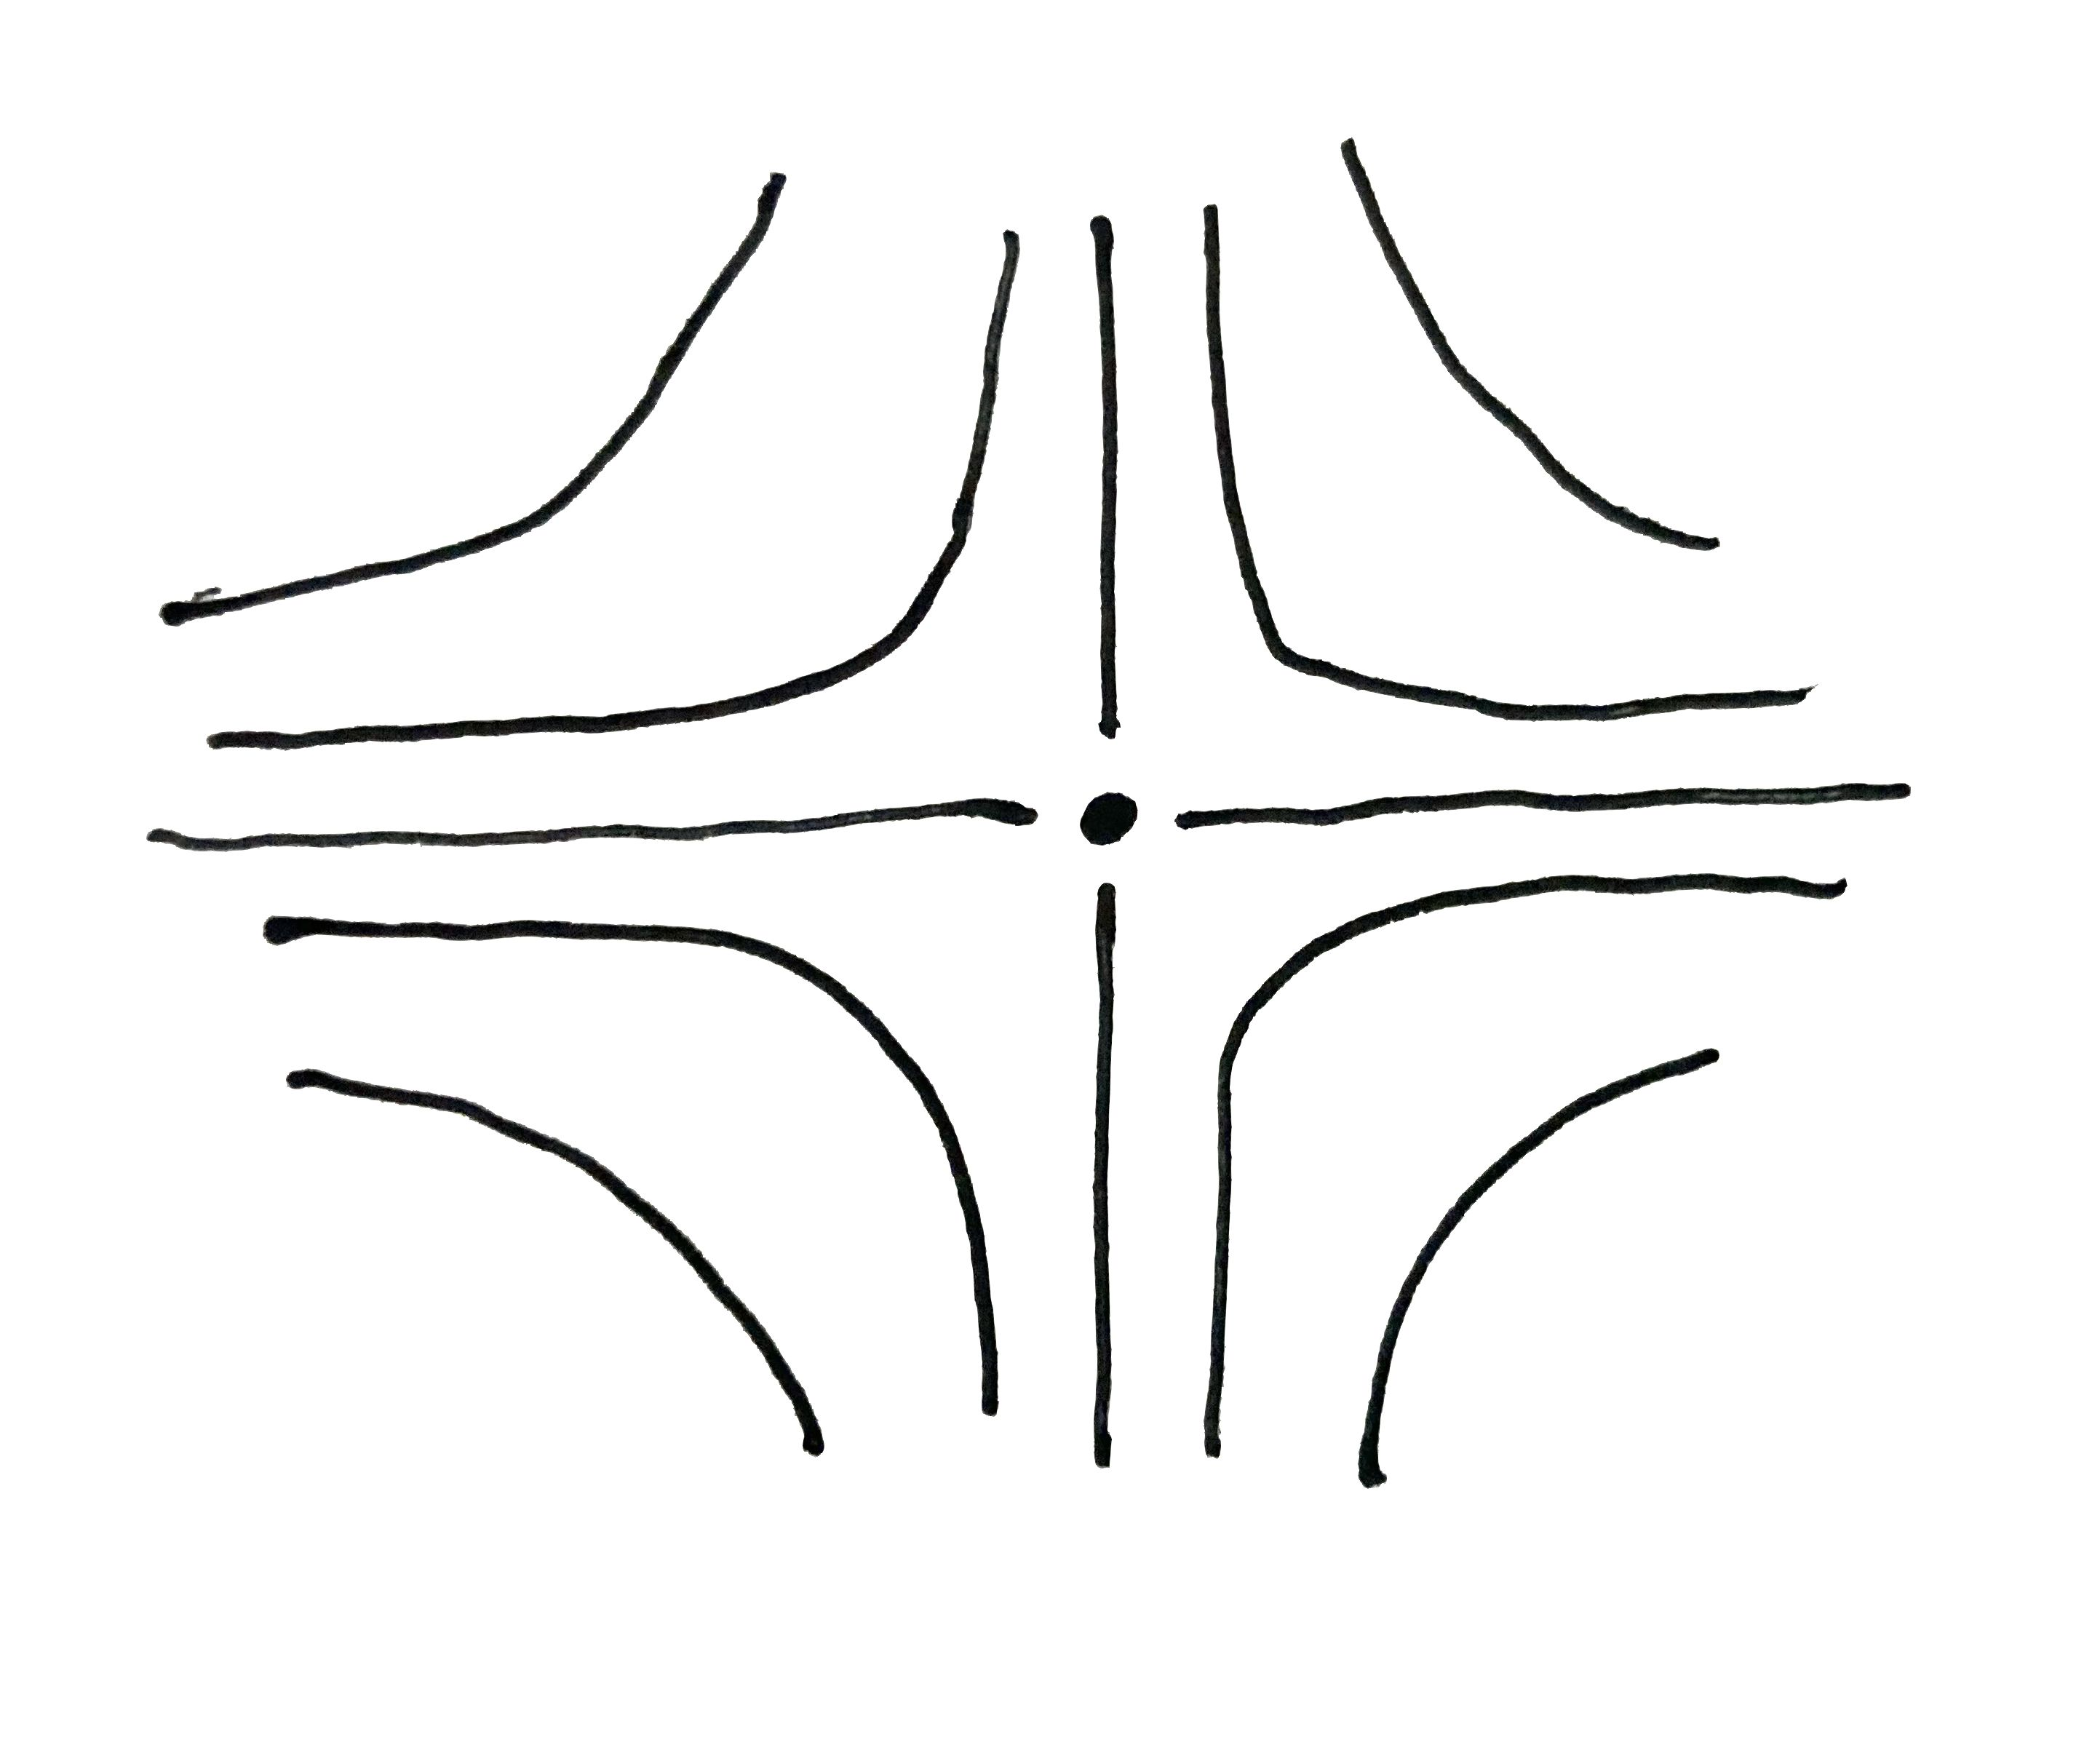
\includegraphics[scale=0.03]{git_saddle}
\end{center}

The typical orbit is $xy=\alpha\in\C^*$, but we also have the $x$-axis with the
origin removed, the $y$-axis with the origin removed, and the origin. Removing
the lower dimensional orbit (the origin) doesn't solve the issue, as the
$x$-axis and $y$-axis cannot be separated from each other. Hence we need some
subtler invariant than dimension.

\paragraph{Affine quotients.} There is a natural construction of ``naive''
algebraic quotients for group actions on affine varieties: the ring of functions
on the quotient should consist of the functions which are invariant under the
action. Hence $X/G=\Spec\,(\O_X)^G$. In the second example above we have
$\C[x,y]^{\C^*}=\C[xy]$, so this gives $\A^1$; the bad orbits are coalesced into
a single point corresponding to $\{xy=0\}$. However, in the first example we
have $\C[x,y]^{\C^*}=\C[x,y]\cap\C(y/x)=\C$, so the quotient is a single point
which is no good.

\paragraph{GIT.} The point of GIT is to provide some subset (the ``unstable
locus'') in a canonical way, so that the GIT quotient
\begin{equation*}
    X\sslash G = (X\setminus\{\text{unstable points}\})/G
\end{equation*}
is well-behaved.

Before defining the unstable locus, we describe a direct construction of the
resulting quotient. From the linearization $G\hookrightarrow\SL(n+1,\C)$ we have
an action $G\curvearrowright H^0(\O_X(r))$ for each $r$. Then
\begin{equation*}
X\sslash G = \Proj\biggl(\bigoplus_{r=0}^\infty H^0(X,\O_X(r))^G\biggr).
\end{equation*}
(The fact that this is a finitely-generated graded ring, so we do get a sensible
projective variety, is a lemma that needs proving.)

To apply this definition in our affine examples, we need to come up with a
``linearization'', i.e. a lift of the $\C^*$ action to some line bundle $L$ over
$\C^n$. Of course, $L$ must be trivial, so we just need to choose a weight for
$\C^*$ to act on one extra coordinate.

\begin{example}
    Consider $\C^*$ acting on $\C^{n+1}$ with weights $(1,\ldots,1)$ as in the
    definition of $\P^n$. Our linearization is a choice of $p\in\Z$ so that
    $\C^*$ acts on the trivial line bundle $L$, total space $\C^{n+1}\times\C$,
    with weights $(1,\ldots,1,p)$. Then $L^{\otimes r}$ has weights
    $(1,\ldots,1,pr)$, and
    \begin{equation*}
        H^0(\C^{n+1},L^{\otimes r})
            = \{\text{degree $pr$ homogeneous polynomials}\}
            = \C[x_0,\ldots,x_n]_{pr},
    \end{equation*}
    so the GIT quotient is
    \begin{equation*}
        \Proj\biggl(\bigoplus_{r=0}^\infty\C[x_0,\ldots,x_n]_{pr}\biggr)
            = \begin{cases*}
                \emptyset & $p<0$, \\
                \text{point} & $p=0$, \\
                \P^n & $p\ge1$.
            \end{cases*}
    \end{equation*}
    Moreover, the line bundle induced by $L$ on the quotient is $\O(p)$.
\end{example}

\subsection*{Stability}

As usual with Proj, we can relate our general construction to concrete
projective embeddings. For each $r\ge0$, the invariant sections
$H^0(X,\O_X(r))^G$ can be evaluated at points of $X$ giving a complex number
defined up to scale, since $\O_X(r)$ is a potentially non-trivial line bundle.
In this way we have a rational map $X\dashrightarrow\P(H^0(X,\O_X(r))^G)^\vee$
given by $x\mapsto[\ev_x]$. (In other language, this is just the map given by
the complete linear system $|\O_X(r)|$.) It is defined only on the locus where
$\ev_x\ne0$, i.e. where there is some invariant section $s\in H^0(X,\O_X(r))^G$
with $s(x)\ne0$.

\begin{claim}
    The GIT quotient $X\sslash G$ is the image of this rational map for $r\gg0$.
\end{claim}

\begin{definition}
    We say $x\in X$ is \emph{semi-stable} if $\exists s\in H^0(X,\O_X(r))^G$
    with $s(x)\ne0$ for $r\gg0$. Otherwise, we say $x$ is \emph{unstable}.
\end{definition}

\begin{claim}
The morphism $X^{ss}=\{\text{semi-stable points}\}\twoheadrightarrow X\sslash G$
is then the usual quotient, so $X\sslash G=X^{ss}/G$.
\end{claim}

\begin{definition}
    We say $x\in X$ is \emph{stable} if $x$ is semi-stable,
    $\bigoplus_{r=0}^\infty H^0(X,\O_X(r))^G$ \emph{separates orbits} near $x$,
    and the stabilizer $\Stab_x$ is finite. (Technically also with an
    infinitesimal version of this condition. We are not intending to thoroughly
    cover technicalities here.)
\end{definition}

What does separating orbits mean? By semi-stability we have
$s\in H^0(X,\O_X(r))^G$ with $s(x)\ne0$, which gives a trivialization of
$\O_X(r)$ on $U=\{s\ne0\}\ni x$; $\O_X(r)|_U\xrightarrow\sim \O_U$. ``Separating
orbits near $x$'' means if $x,y\in U$ are in distinct orbits then some function
on $U$ vanishes at $x$ but not $y$.

We then have $X^s\subseteq X^{ss}\twoheadrightarrow X\sslash G$, and the
restriction $X^s\to X\sslash G$ is ``good'' in the sense that only 1 orbit is
collapsed for each point in the image.

\begin{example}
    Consider $\C^*$ acting on $\C^2$ by
    $\lambda\cdot(x,y)=(\lambda x,\lambda^{-1}y)$. The single orbits $xy=\alpha$
    for $\alpha\ne0$ give the stable locus, while $xy=0$ which contains 3 orbits
    only consists of semistable points.
\end{example}

\subsection*{Hilbert--Mumford stability criterion}

Working in upstairs in the line bundle $\O_X(-1)$, we have a clean
characterization of stability. Take $\tilde x$ to be a lift of $x\in X$ to the
total space of $\O_X(-1)$. Then:
\begin{itemize}
    \item $x$ is semi-stable iff $\closure{G\cdot\tilde x}$ does not contain the
        origin of any fibre.
    \item $x$ is stable iff $G\cdot\tilde x$ is closed with finite stabilizer.
\end{itemize}

We can optimize this criterion further. Consider an arbitrary 1-parameter
subgroup $\C^*\le G$. For $x\in X$, the orbit under this subgroup has a limit
$x_0=\lim_{\lambda\to0,\lambda\in\C^*}\lambda\cdot x$, which is a
fixed point of $\C^*$. This then gives us a weight $\rho\in\Z$ for the action of
$\C^*$ on the fiber $\O_X(-1)|_{x_0}$.

\begin{theorem}[Hilbert--Mumford]
    \begin{itemize}
        \item  If $\rho\le0$ for all 1-parameter subgroups then $x$ is
            semi-stable.
        \item If $\rho<0$ for all 1-parameter subgroups then $x$ is stable.
        \item Otherwise, $x$ is unstable.
    \end{itemize}
\end{theorem}

\subsection*{Exercises}

\begin{enumerate}
    \item Consider $\P^n=\C^{n+1}\sslash\C^*$ again. Use the criterion to check
        that $\{0\}$ is the unstable locus.

    \item Consider $(\C^*)^2$ acting on $\C^4$ with weights $\begin{pmatrix}
            1 & 1 & 0 & -1 \\ 0 & 0 & 1 & 1
    \end{pmatrix}$. Take the linearization which gives weights $(-a,-b)$ to the
    trivial line bundle.
        \begin{enumerate}
            \item Set $a=b=1$. Show that the unstable locus is
                $\{x=y=0\}\cup\{z=w=0\}$. Write $X_+=X^{ss}/(\C^*)^2$, and show
                that it is a $\P^1$-bundle over $\P^1$, $\P(\O\oplus\O(-1))$,
                the blowup of $\P^2$ at a point.

            \item Set $a=-1$, $b=2$. Show that the unstable locus is
                $\{x=y=z=0\}\cup\{w=0\}$. Write $X_-=X^{ss}/(\C^*)^2$, and show
                that $X_-\cong\P^2$.

            \item Say VGIT: $X_\pm$ are both $\C^4\setminus\{\cdots\}/(\C^*)^2$,
                giving a birational map between them. (Blow-up!)
        \end{enumerate}

    \item Construct the Grassmannian $\Gr(k,N)$ as a GIT quotient.
\end{enumerate}

\section{Morse Theory - Mikhail Karpukhin}

The basic setup: we have a compact\footnote{For many things we say here
compactness isn't crucial} $n$-manifold, and a smooth function $f:M\to\R$. The
idea is to study the topology of $M$ using $f$; using the critical points
\begin{equation*}
    \Crit(f) = \{p\in M:\text{$p$ critical point of $f$}\},
\end{equation*}
and the sub-level sets
\begin{equation*}
    M^c = f^{-1}(-\infty,c) = \{x\in M:f(x)<c\}.
\end{equation*}

The following are some important examples of this setup, which we will keep
revisiting. For a manifold drawn in Euclidean space we take the height function
as our $f$.

\begin{center}
    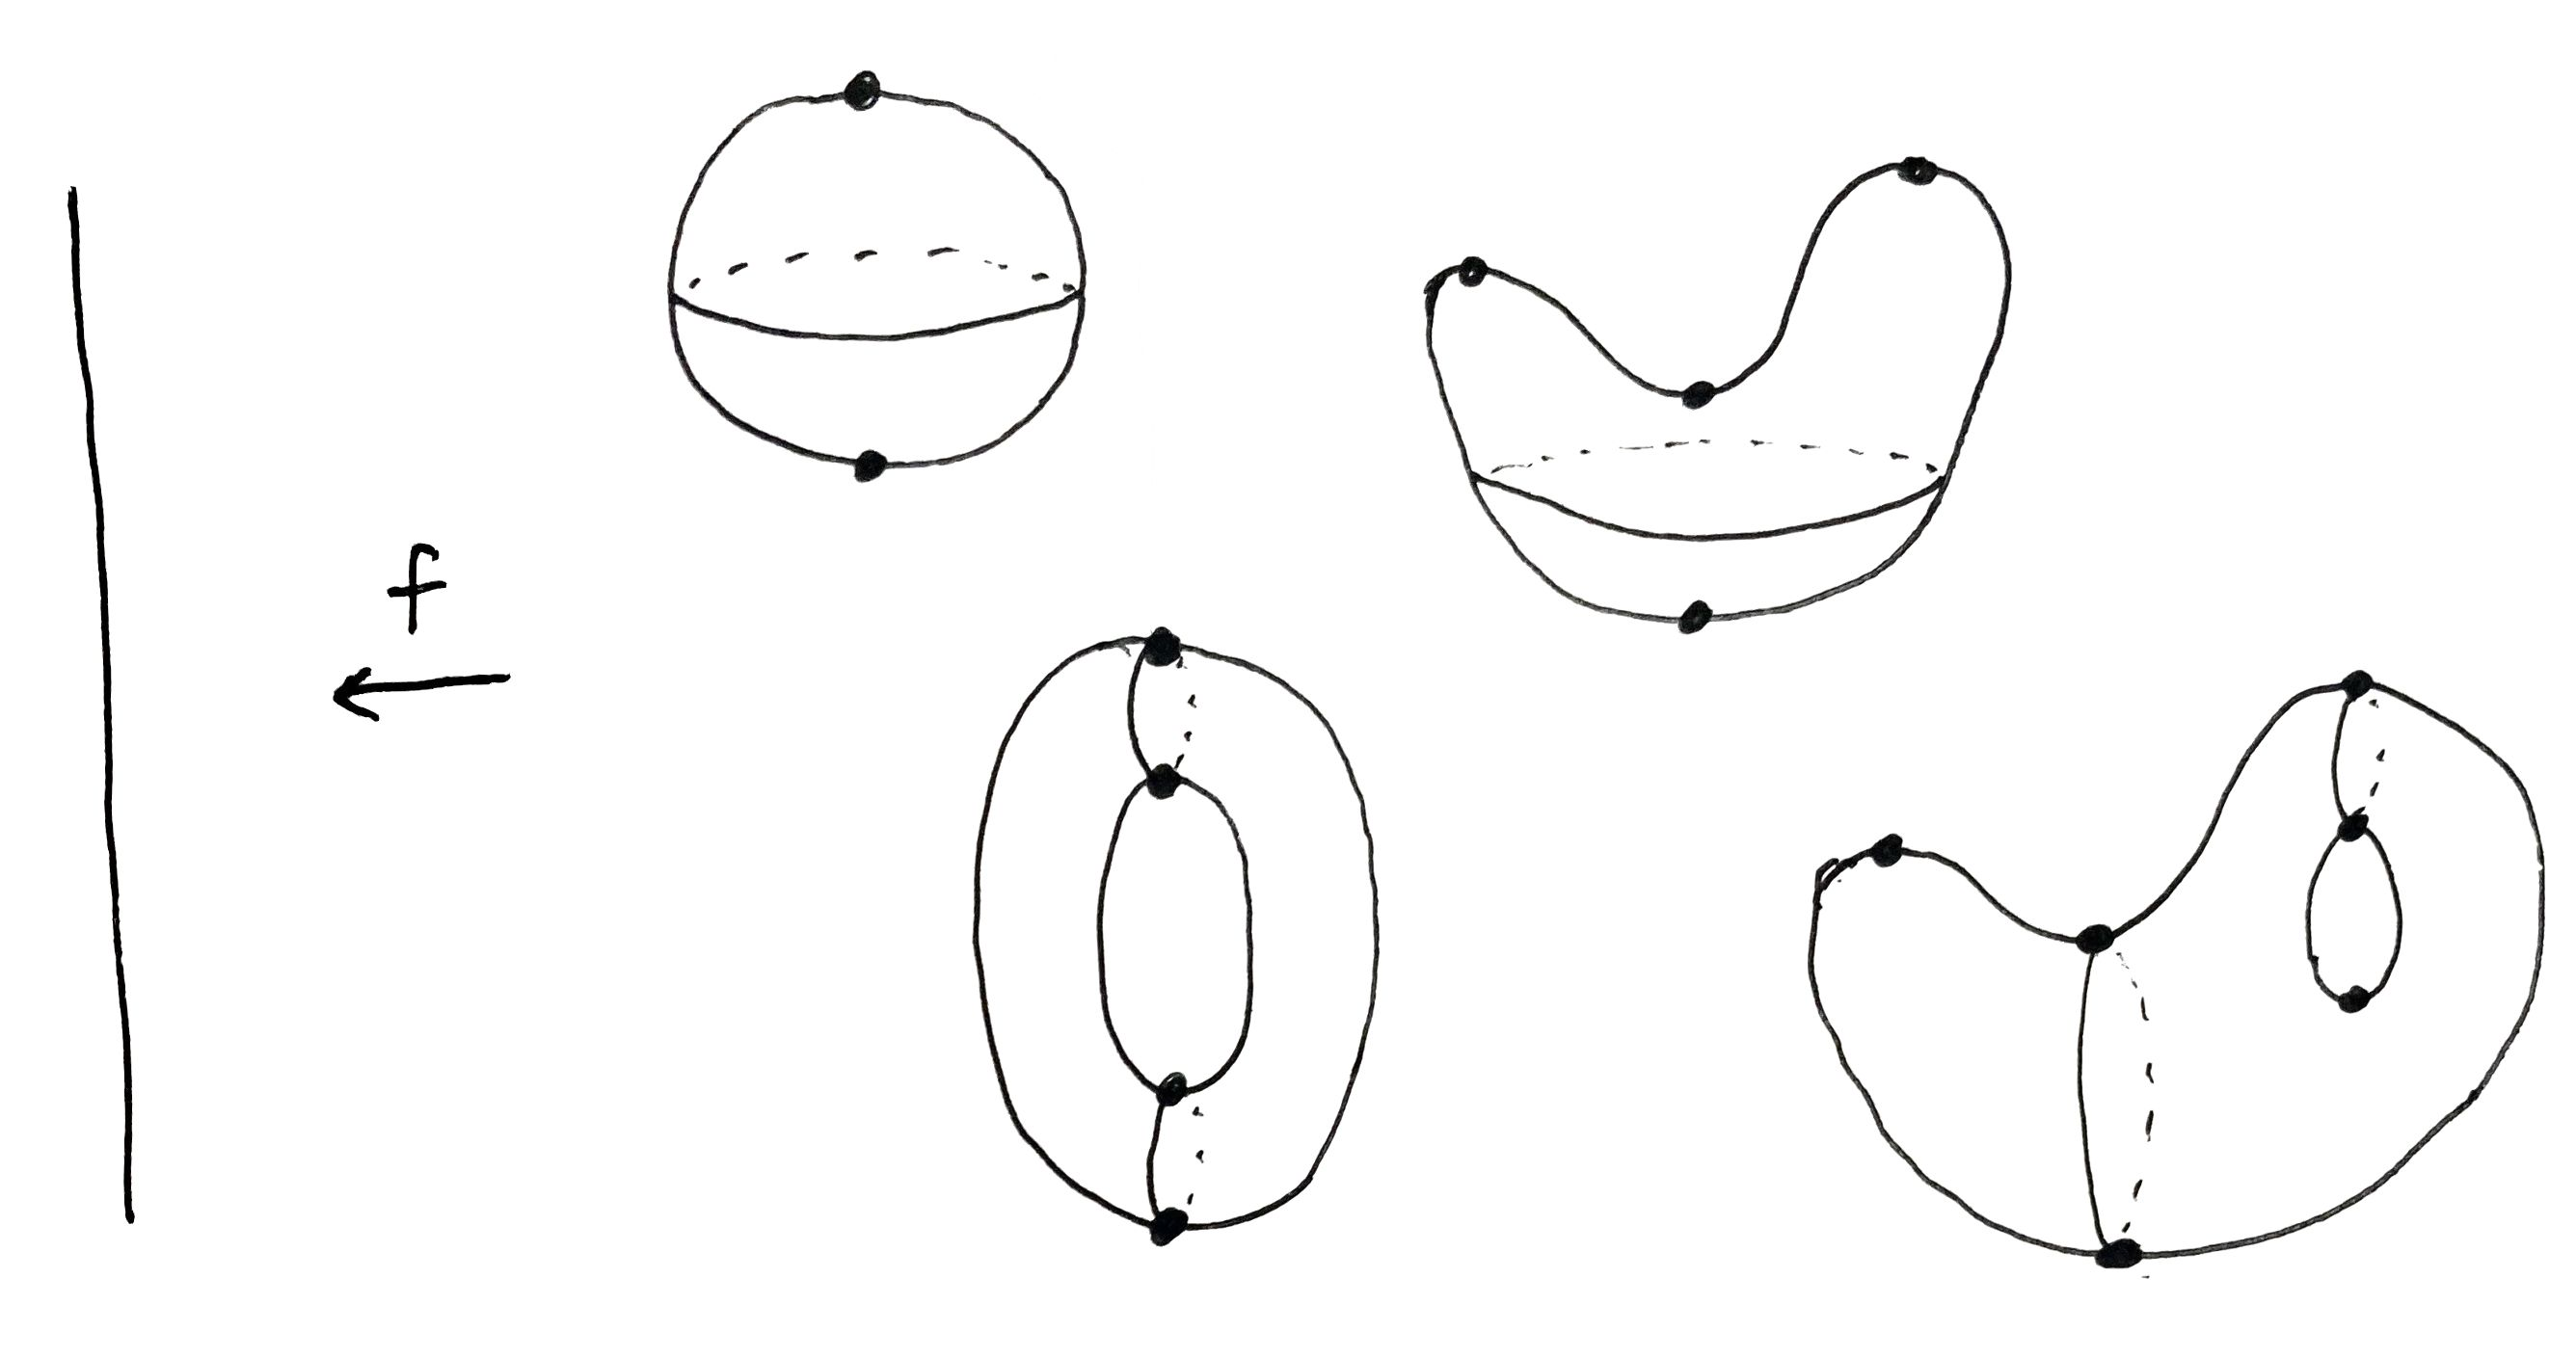
\includegraphics[scale=0.13]{morse_examples}
\end{center}

\subsection*{Plan / Overview}

\begin{itemize}
    \item Describe computation of the homology $H_k(M)$ using $f$ (Morse
        homology).

    \item Mention contemporary research in Morse theory; applying inspired ideas
        to infinite-dimensional manifolds. (For example solutions to PDE's are
        often characterized as critical points of certain functionals on
        infinite-dimensional function spaces.)
\end{itemize}

\subsection*{References}

\begin{itemize}
    \item ``Morse Theory'', Milnor
    \item ``Morse Theory and Floer Homology'', Audin and Damian
\end{itemize}
For a complete treatment of the basic theory, and applications to Riemannian
geometry (e.g. length functional on geodesics) see Milnor, but for the
homological treatment and connections to symplectic geometry see Audin and
Damian.

\subsection*{Critical points}

\begin{definition}
    A \emph{critical point} $p\in M$ of $f$ is a point where $df_p=0$ in $T_pM$.
\end{definition}

Take a metric $g$ on $M$. We define the gradient vector field $\nabla f$ by
$\langle\nabla f,X\rangle=df(X)$. Then $p$ is a critical point iff
$\nabla f(p)=0$. The flow lines of $-\nabla f$ give trajectories along which a
drop of water placed on the manifold would run down.
\begin{center}
    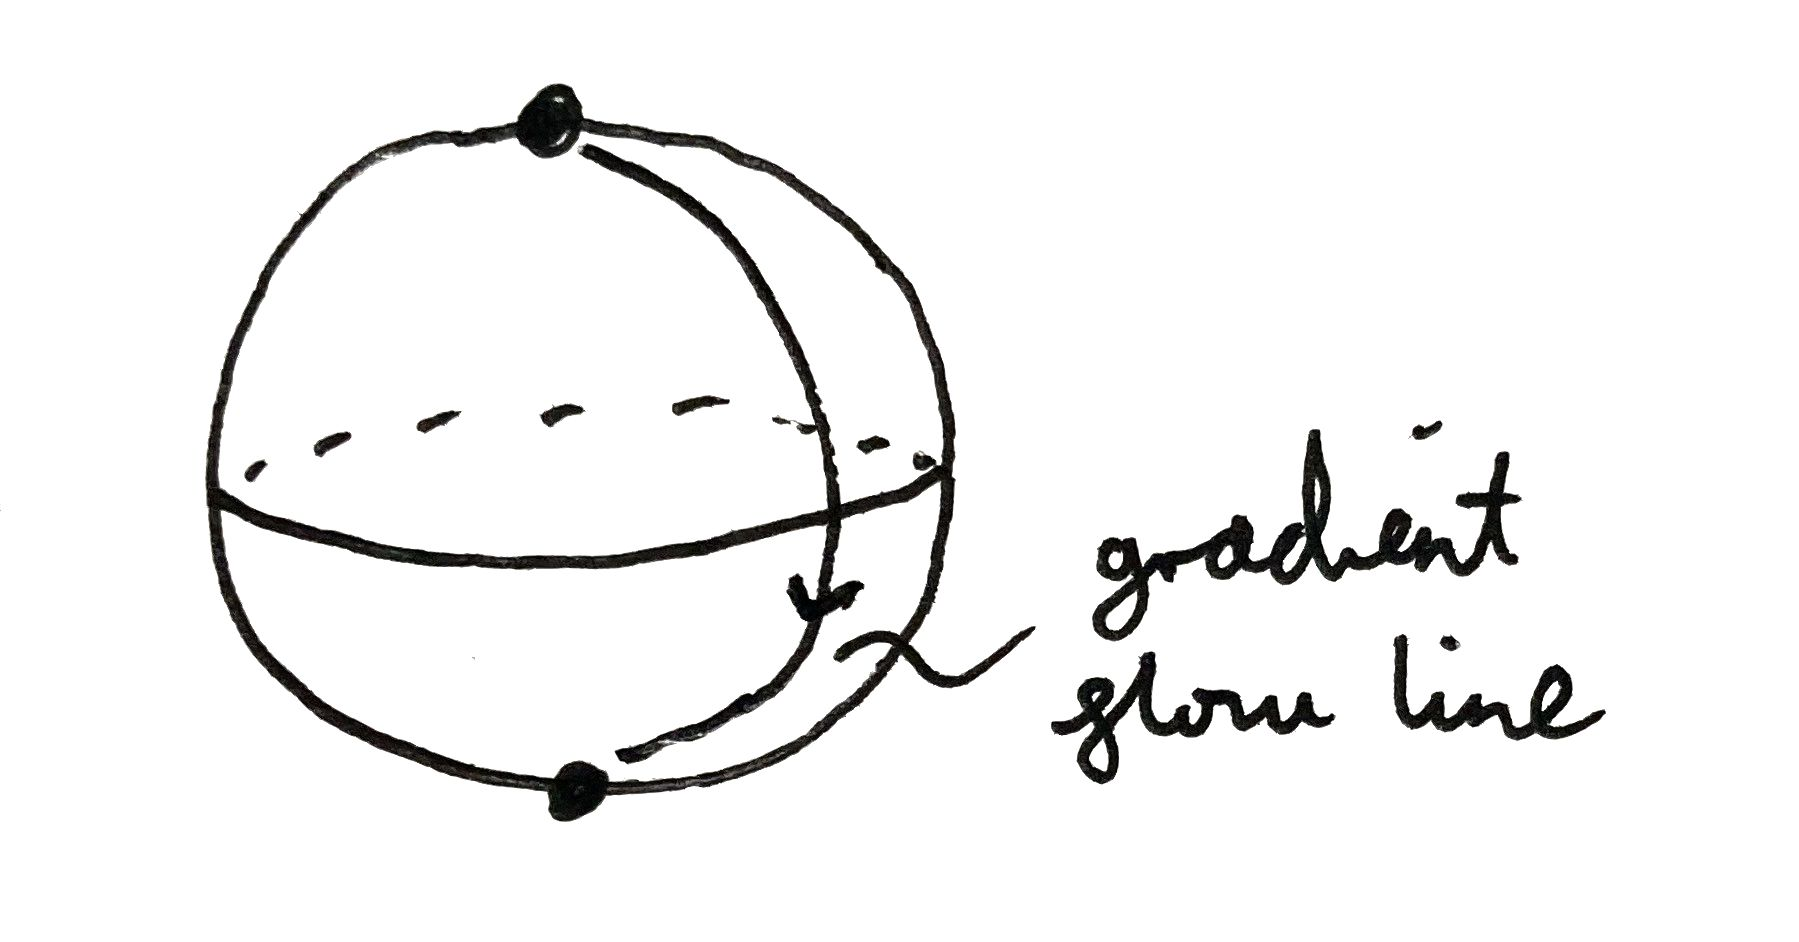
\includegraphics[scale=0.1]{morse_flow}
\end{center}
Why do we care about $\Crit(f)$? Because of the following:

\begin{proposition}
    If $f^{-1}[a,b]$ contains no critical points, then $M^a\cong_\diffeo M^b$.
\end{proposition}

\begin{proof}
    Define via bump functions
    \begin{equation*}
        \rho(x) = \begin{dcases*}
            \frac{1}{|\nabla f|^2} & on $f^{-1}[a,b]$ \\
            0 & outside some neighbourhood of $f^{-1}[a,b]$,
        \end{dcases*}
    \end{equation*}
    and consider the vector field $X=-\rho\cdot\nabla f$ with flow $\varphi_t$
    globally defined by compactness. If $\varphi_t(q)\in f^{-1}[a,b]$ for small
    $t$, then
    \begin{equation*}
        \odv{}{t}\biggr\vert_{t=0}f(\varphi_t(q))
            = \langle\nabla f,X(q)\rangle
            = -\rho(q)|\nabla f(q)|^2
            = -1.
    \end{equation*}
    Then by integrating, $\varphi_{b-a}$ maps $M^b\to M^a$ and is a
    diffeomorphism by construction.
\end{proof}

So if we want to build up the topology on $M$ from the sub-level sets $M^t$, we
need to understand how the topology of $M^t$ changes as $t$ passes through
critical values of $f$. (Think about how this applies in the main examples.)

\begin{center}
    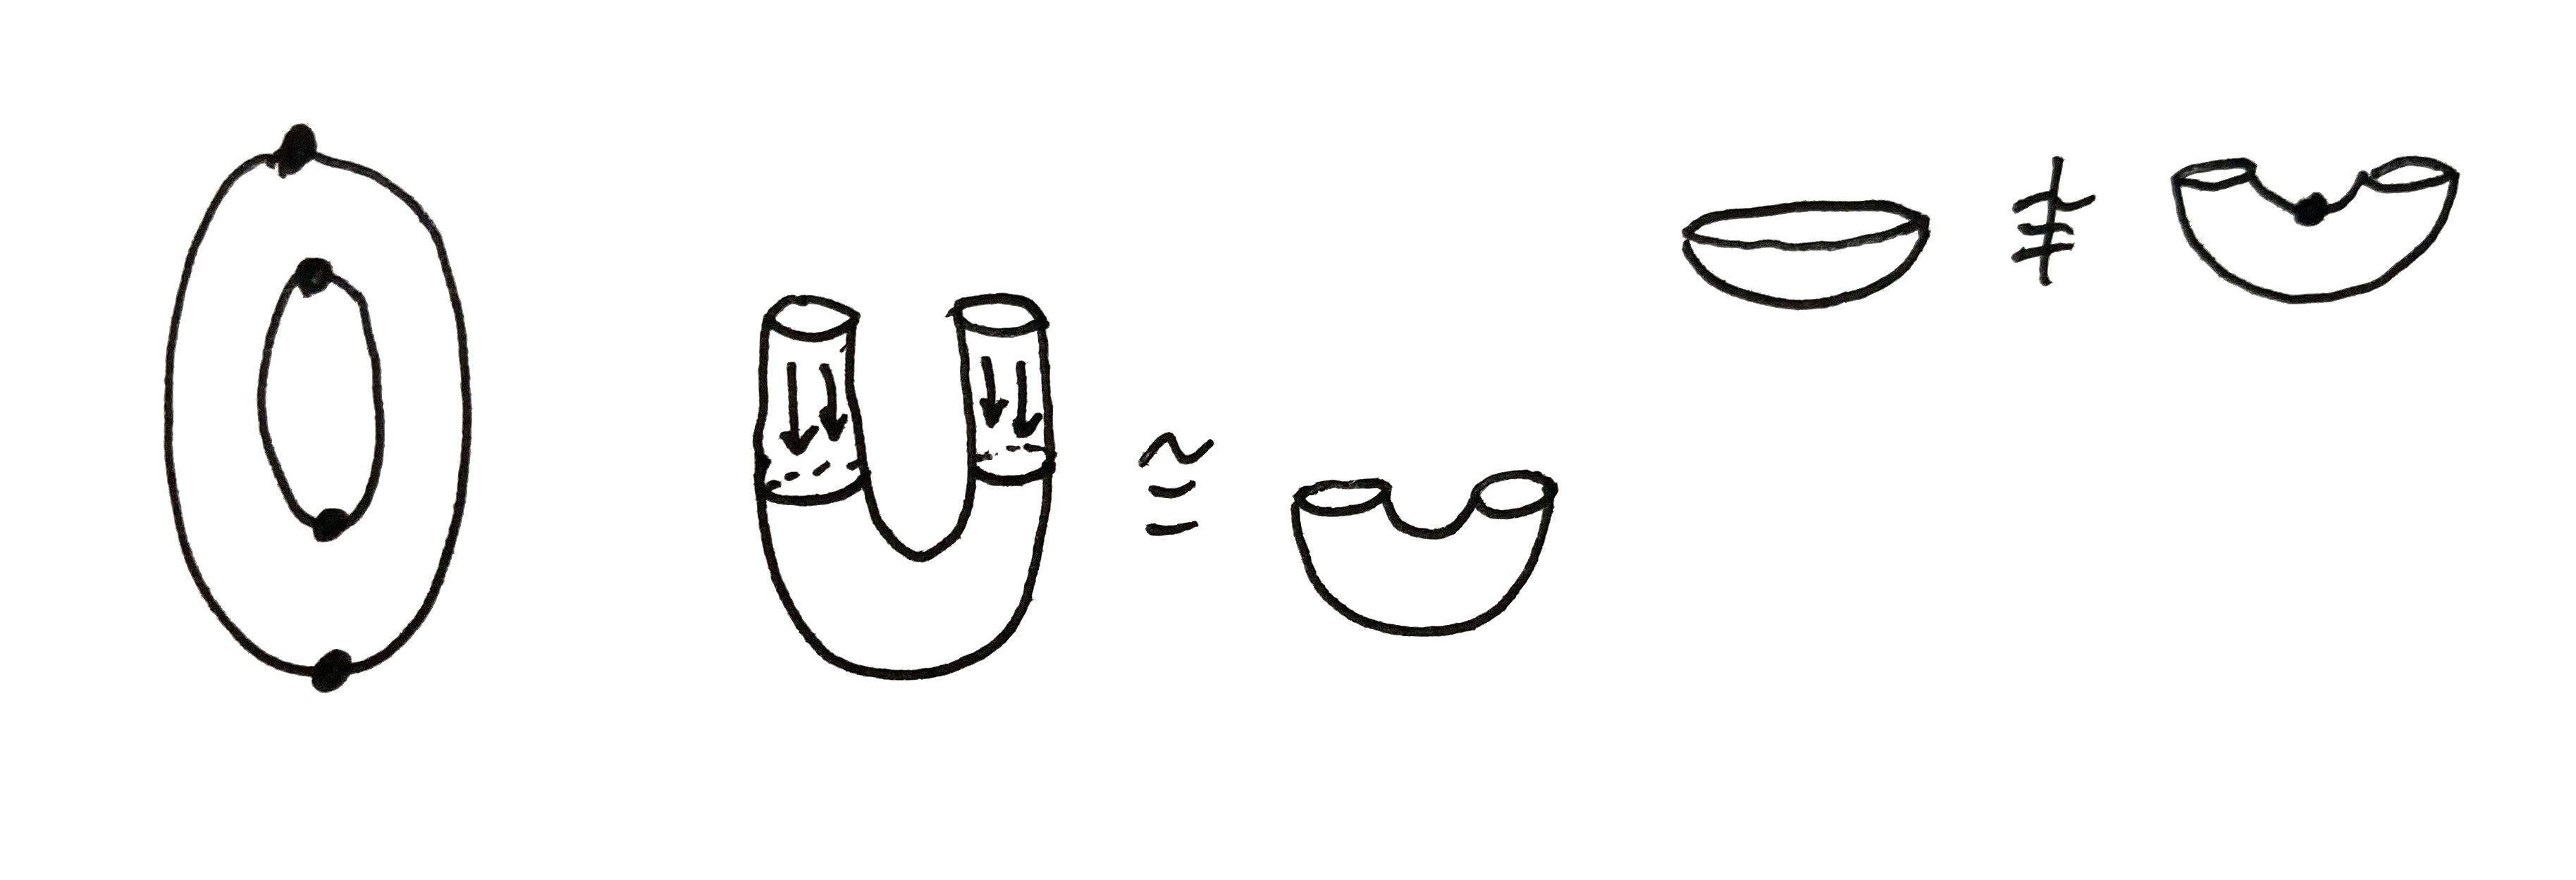
\includegraphics[scale=0.1]{morse_steps}
\end{center}

\subsection*{Morse functions}

To this end, fix a critical point $p\in\Crit(f)$, with $f(p)=c$. Suppose for
simplicity that $f^{-1}(c)\cap\Crit(f)=\{p\}$. (This is true in our main
examples, and is not a serious restriction.)

Our idea is that the interesting behaviour occurs in a neighbourhood of $p$,
where the gradient flow breaks down, and so we want $f$ to be easy to analyse
(e.g. via Taylor expansion) near $p$.

\begin{definition}
    For $p\in\Crit(f)$, the \emph{Hessian} $\Hess_p(f)$ is a bilinear form on
    $T_pM$ given by
    \begin{equation*}
        (X,Y) \mapsto X(\widetilde Y(f)),
    \end{equation*}
    where $\widetilde Y$ is any extension of $Y$ to a vector field in a
    neighbourhood of $p$. It is well-defined and symmetric, given in local
    coordinates by
    \begin{equation*}
        \begin{pmatrix}
            \pdv{f}{x_1,x_1} & \cdots & \\
            \cdots & \pdv{f}{x_i,x_j} & \cdots \\
                   & \cdots & \pdv{f}{x_n,x_n}
        \end{pmatrix}.
    \end{equation*}
\end{definition}

\begin{definition}
    A critical point $p\in\Crit(f)$ is \emph{non-degenerate} if
    $\Hess_p(f)$ is a non-degenerate bilinear form.
\end{definition}

\begin{definition}
    The function $f$ is \emph{Morse} if all its critical points are
    non-degenerate.
\end{definition}

\begin{lemma}[Morse Lemma]
    Let $p\in\Crit(f)$ be non-degenerate. Then there exists some coordinate
    system in a neighbourhood of $p$ such that
    \begin{equation*}
        f(x) = f(p)
            + x_1^2 + \cdots + x_{n-i}^2 - (x_{n-i+1}^2 + \cdots + x_n^2).
    \end{equation*}
\end{lemma}

\begin{proof}[Sketch proof]
    We have $f(x)-f(p)=\int_0^1\odv{}{t}f(tx)dt
    =\sum_ix_i\int_0^1\pdv{f}{x_i}(tx)dt=\sum_ix_ig_i(x)$, with $g_i(p)=0$.
    Applying this to each $g_i$ gives $f(x)=f(p)+\sum_{i,j}x_ix_jh_{ij}(x)$ with
    $\Hess_p(f)=(h_{ij}(p))$. We then bring this to the desired form using a
    change of variables akin to diagonalization of the bilinear form
    $\Hess_p(f)$.
\end{proof}

(See Milnor's book for a proper proof.)

\begin{definition}
    The \emph{index} of $p$ is $\ind_p(f)=i$, which is uniquely determined as
    the number of negative eigenvalues of the Hessian.
\end{definition}

Using this, we can understand how the topology of $M^c$ changes as we pass
through a non-degenerate critical point:

\begin{center}
    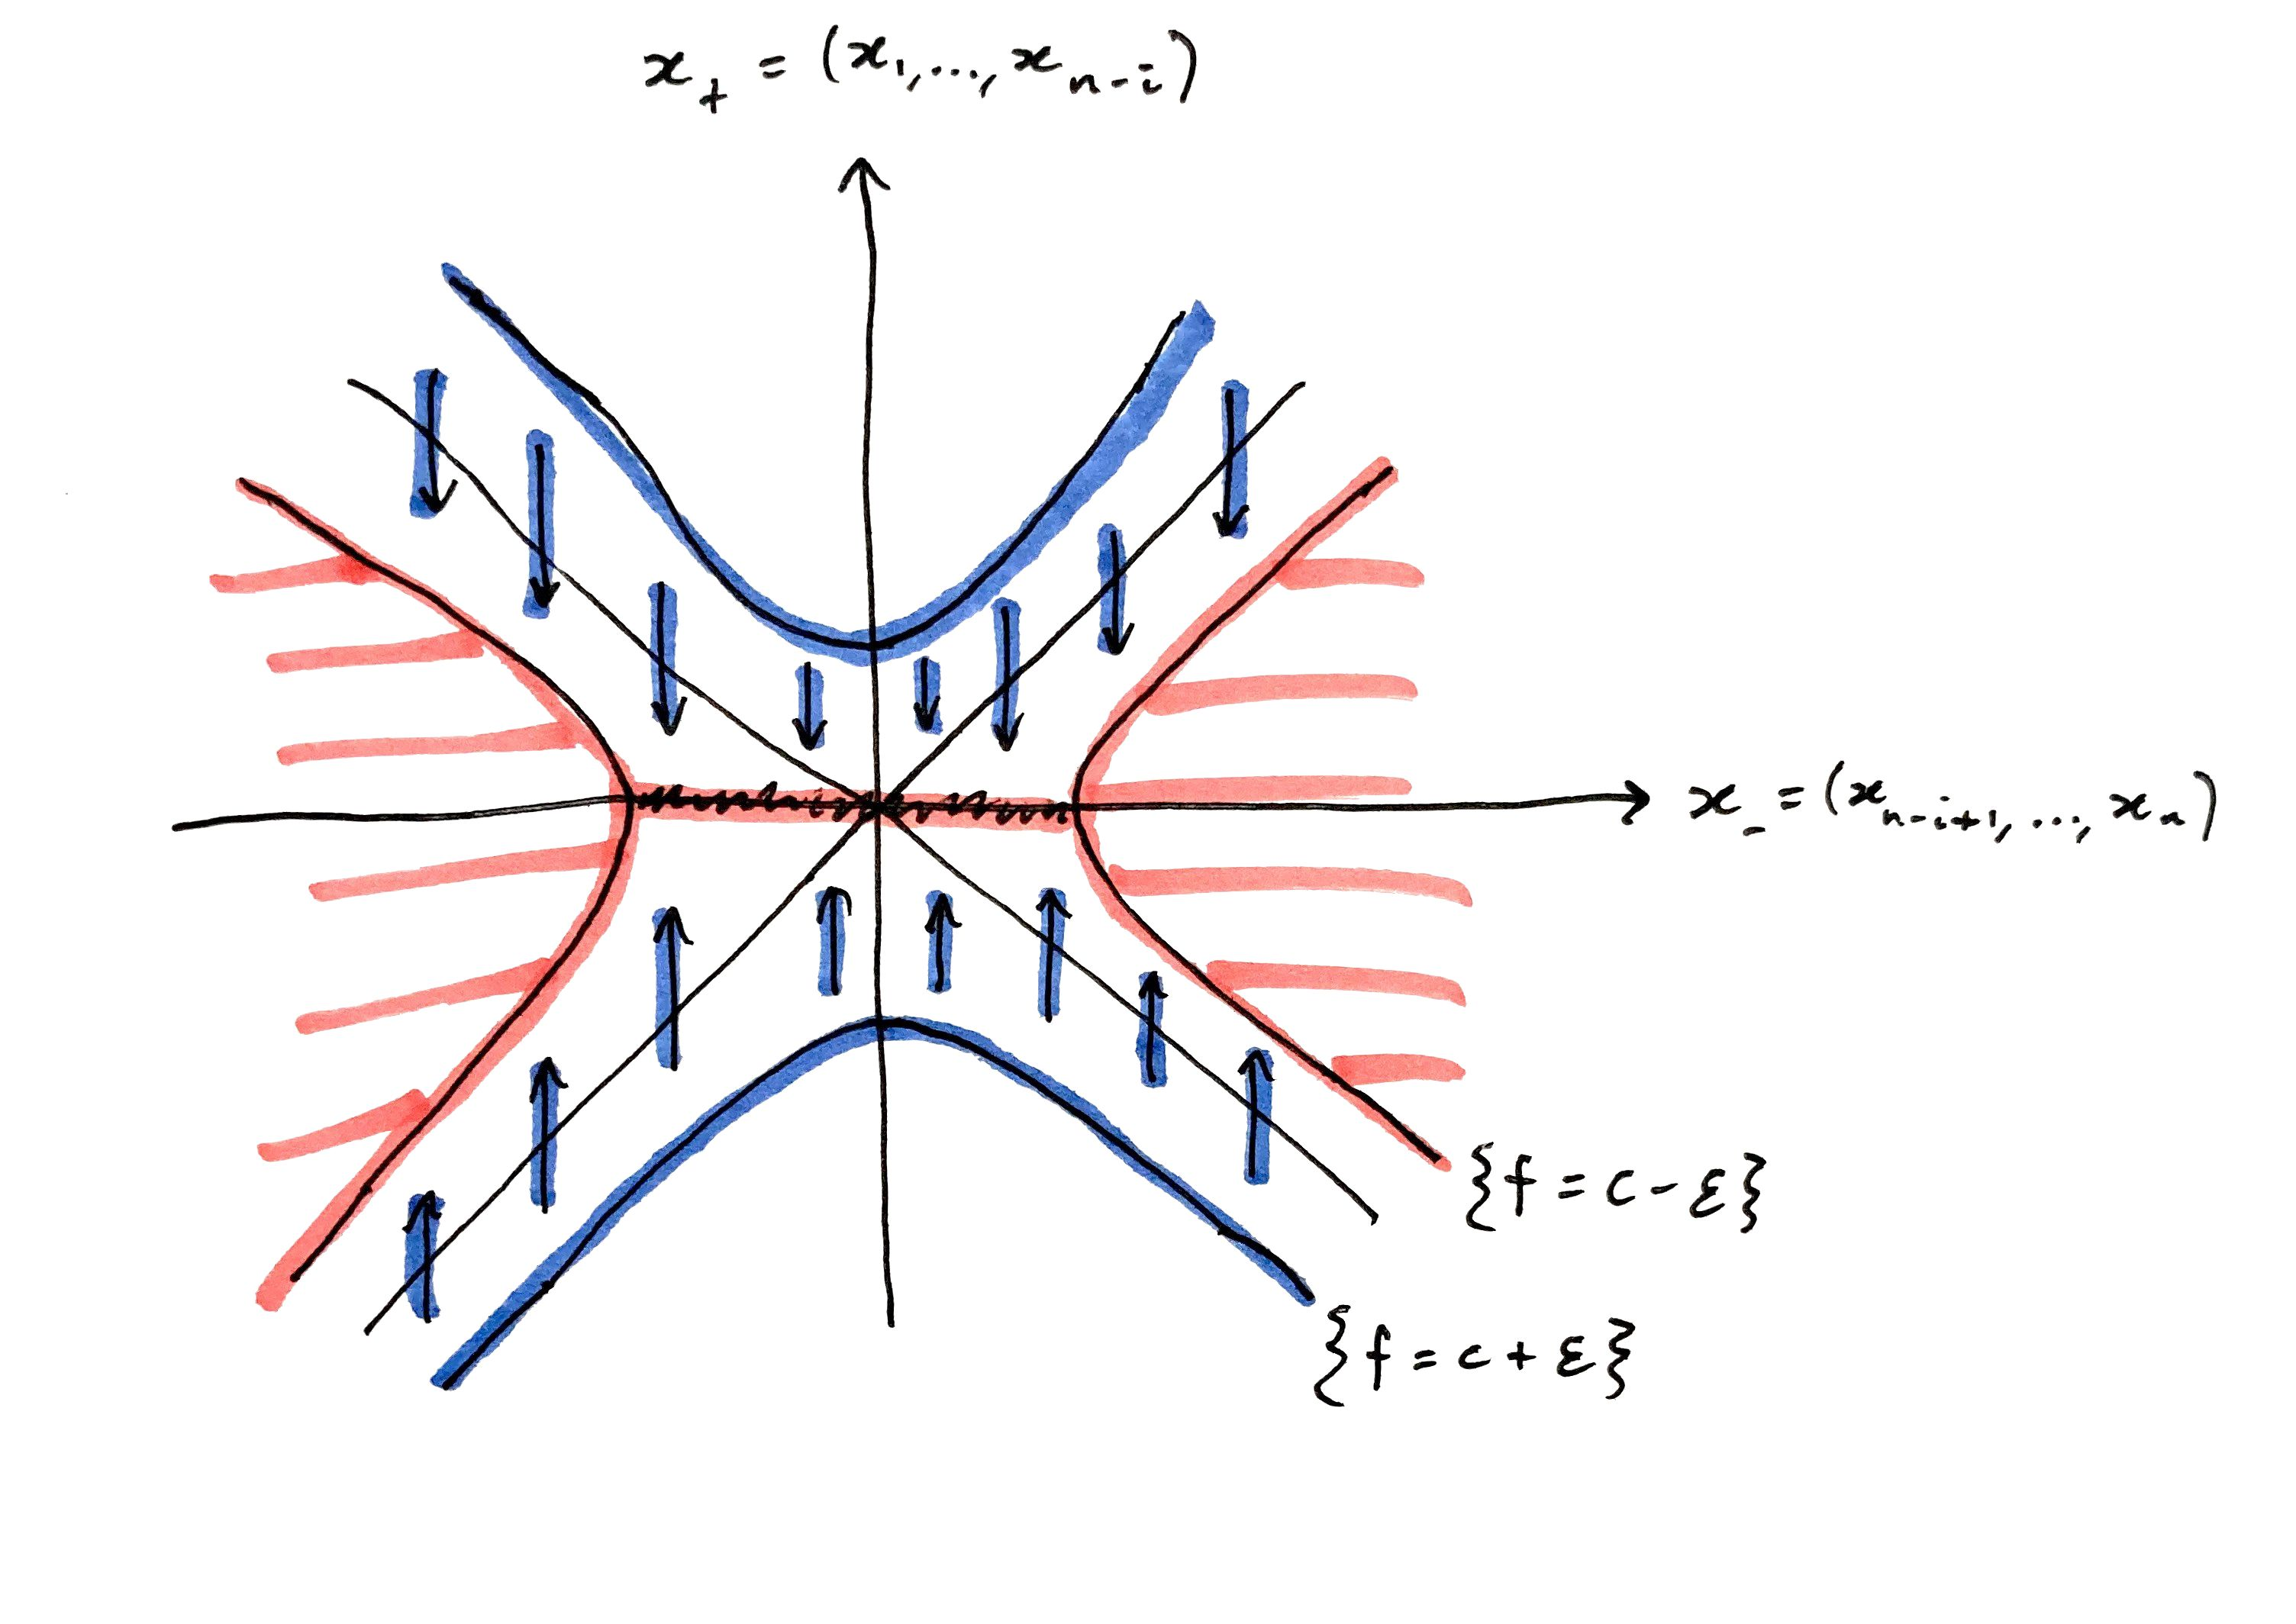
\includegraphics[scale=0.13]{morse_model}
\end{center}

By a similar argument to the gradient flow from before, we see that
$M^{c+\varepsilon}$ is obtained from $M^{c-\varepsilon}$ by attaching a
thickening of the $i$-cell where $x_+=0$.

\begin{theorem}
    Suppose that $f^{-1}[a,b]$ contains a single non-degenerate critical point.
    Then
    \begin{equation*}
        M^b \approx_\homeo M^a \cup_{S^i\times D^{n-i}}D^i\times D^{n-i}.
    \end{equation*}
    Up to homotopy equivalence $M^b$ is given by attaching an $i$-cell to $M^a$.
\end{theorem}

\begin{remark}
    The only reason we have a homeomorphism rather than a diffeomorphism is that
    the naive attachment of a thickened $i$-cell has corners and hence is not
    smooth. It is possible to choose a canonical way to smooth these corners up
    to diffeomorphism, leading to the notion of handle attachment for smooth
    manifolds, and then the theorem carries over.
\end{remark}

We can check how this works out in our main examples:

\begin{center}
    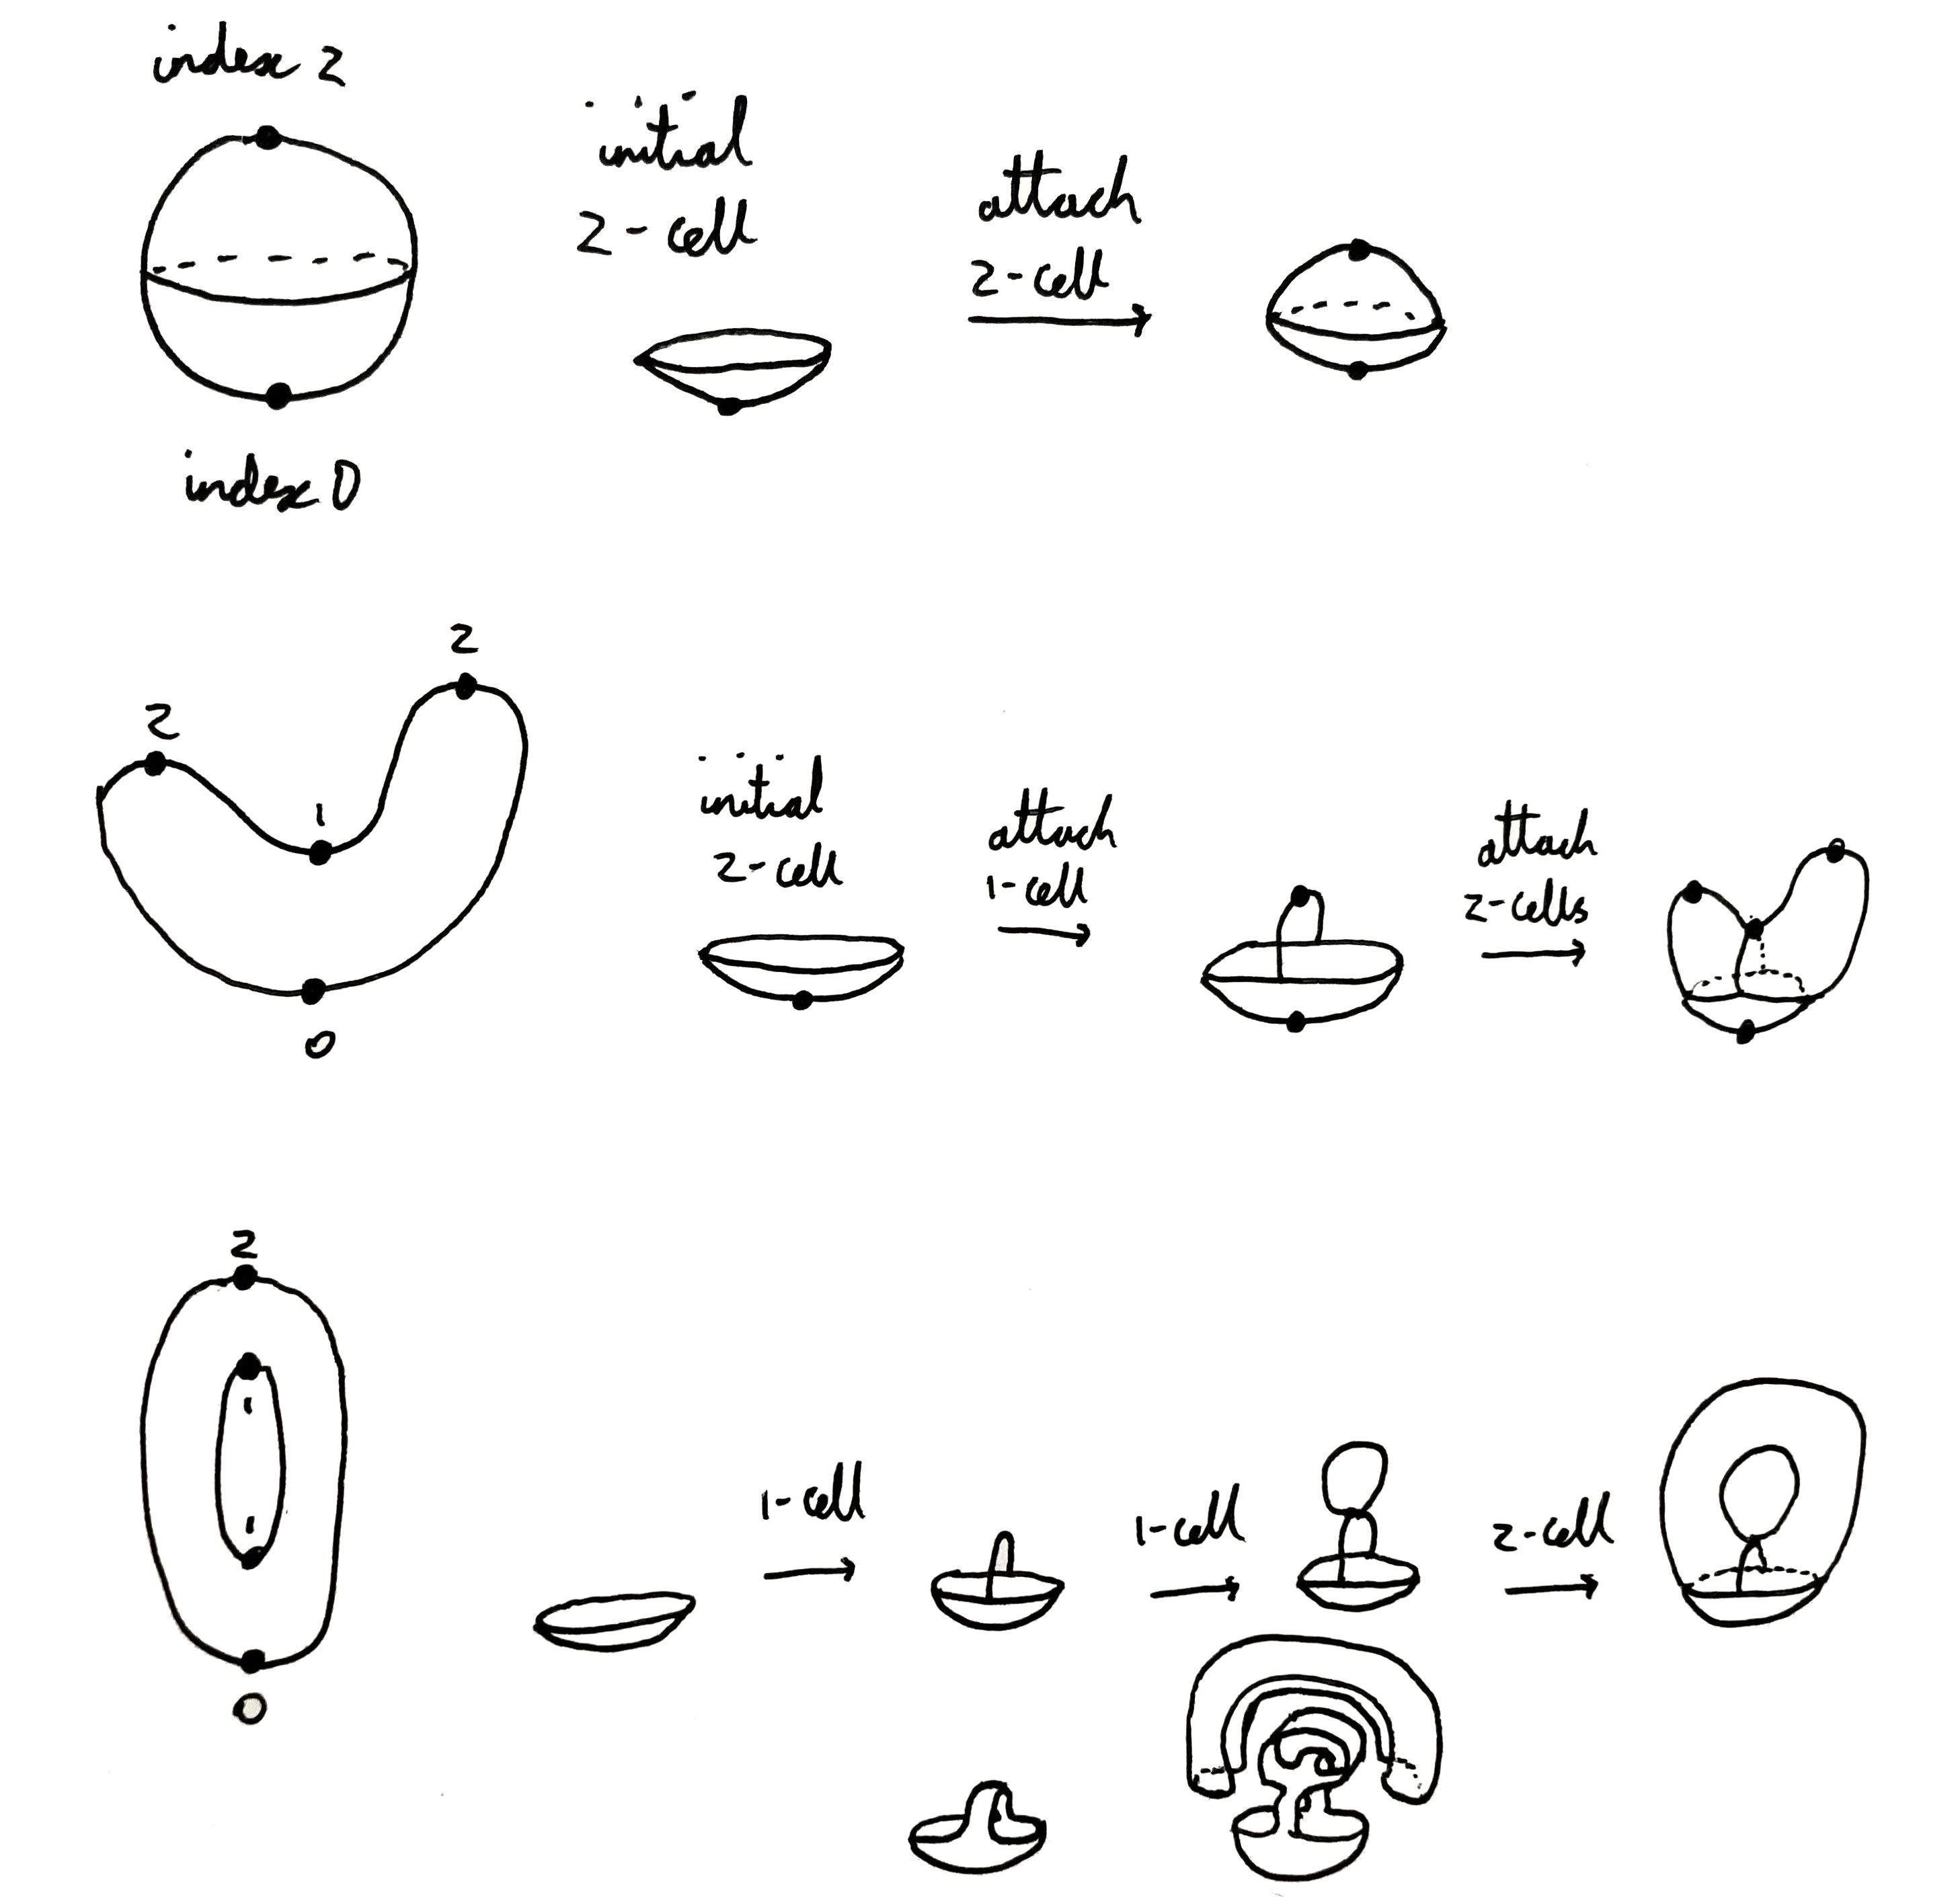
\includegraphics[scale=0.14]{morse_cells}
\end{center}

\begin{theorem}
    A generic (in the sense of Baire category) smooth function on a compact
    manifold is Morse.
\end{theorem}

\begin{remark}
    The assumption $f^{-1}(c)\cap\Crit(f)=\{p\}$ is also true generically.
\end{remark}

\begin{corollary}
    Every compact manifold is homotopy equivalent to a cell complex.
\end{corollary}

\subsection*{Morse homology}

From now on we assume $f$ is a Morse function (with distinct critical values).

To extract quantitative information about the topology from a given Morse
function, we want to understand how this cell decomposition works in more
detail. To construct the chain complex computing cellular homology we want to
know what the boundaries of the attached $i$-cells are in terms of $f$, and to
this end we want an intrinsic characterization of the cell decomposition.

\begin{definition}
    For $p\in\Crit(f)$, let $\varphi_t$ be the flow of $-\nabla f$. The
    \emph{unstable manifold} at $p$ is
    \begin{equation*}
        W^u(p) = \{x\in M:\lim_{t\to\infty}\varphi_t(x)=p\},
    \end{equation*}
    and the \emph{stable manifold} is
    \begin{equation*}
        W^s(p) = \{x\in M:\lim_{t\to-\infty}\varphi_t(x)=p\}.
    \end{equation*}
\end{definition}

For example:

\begin{center}
    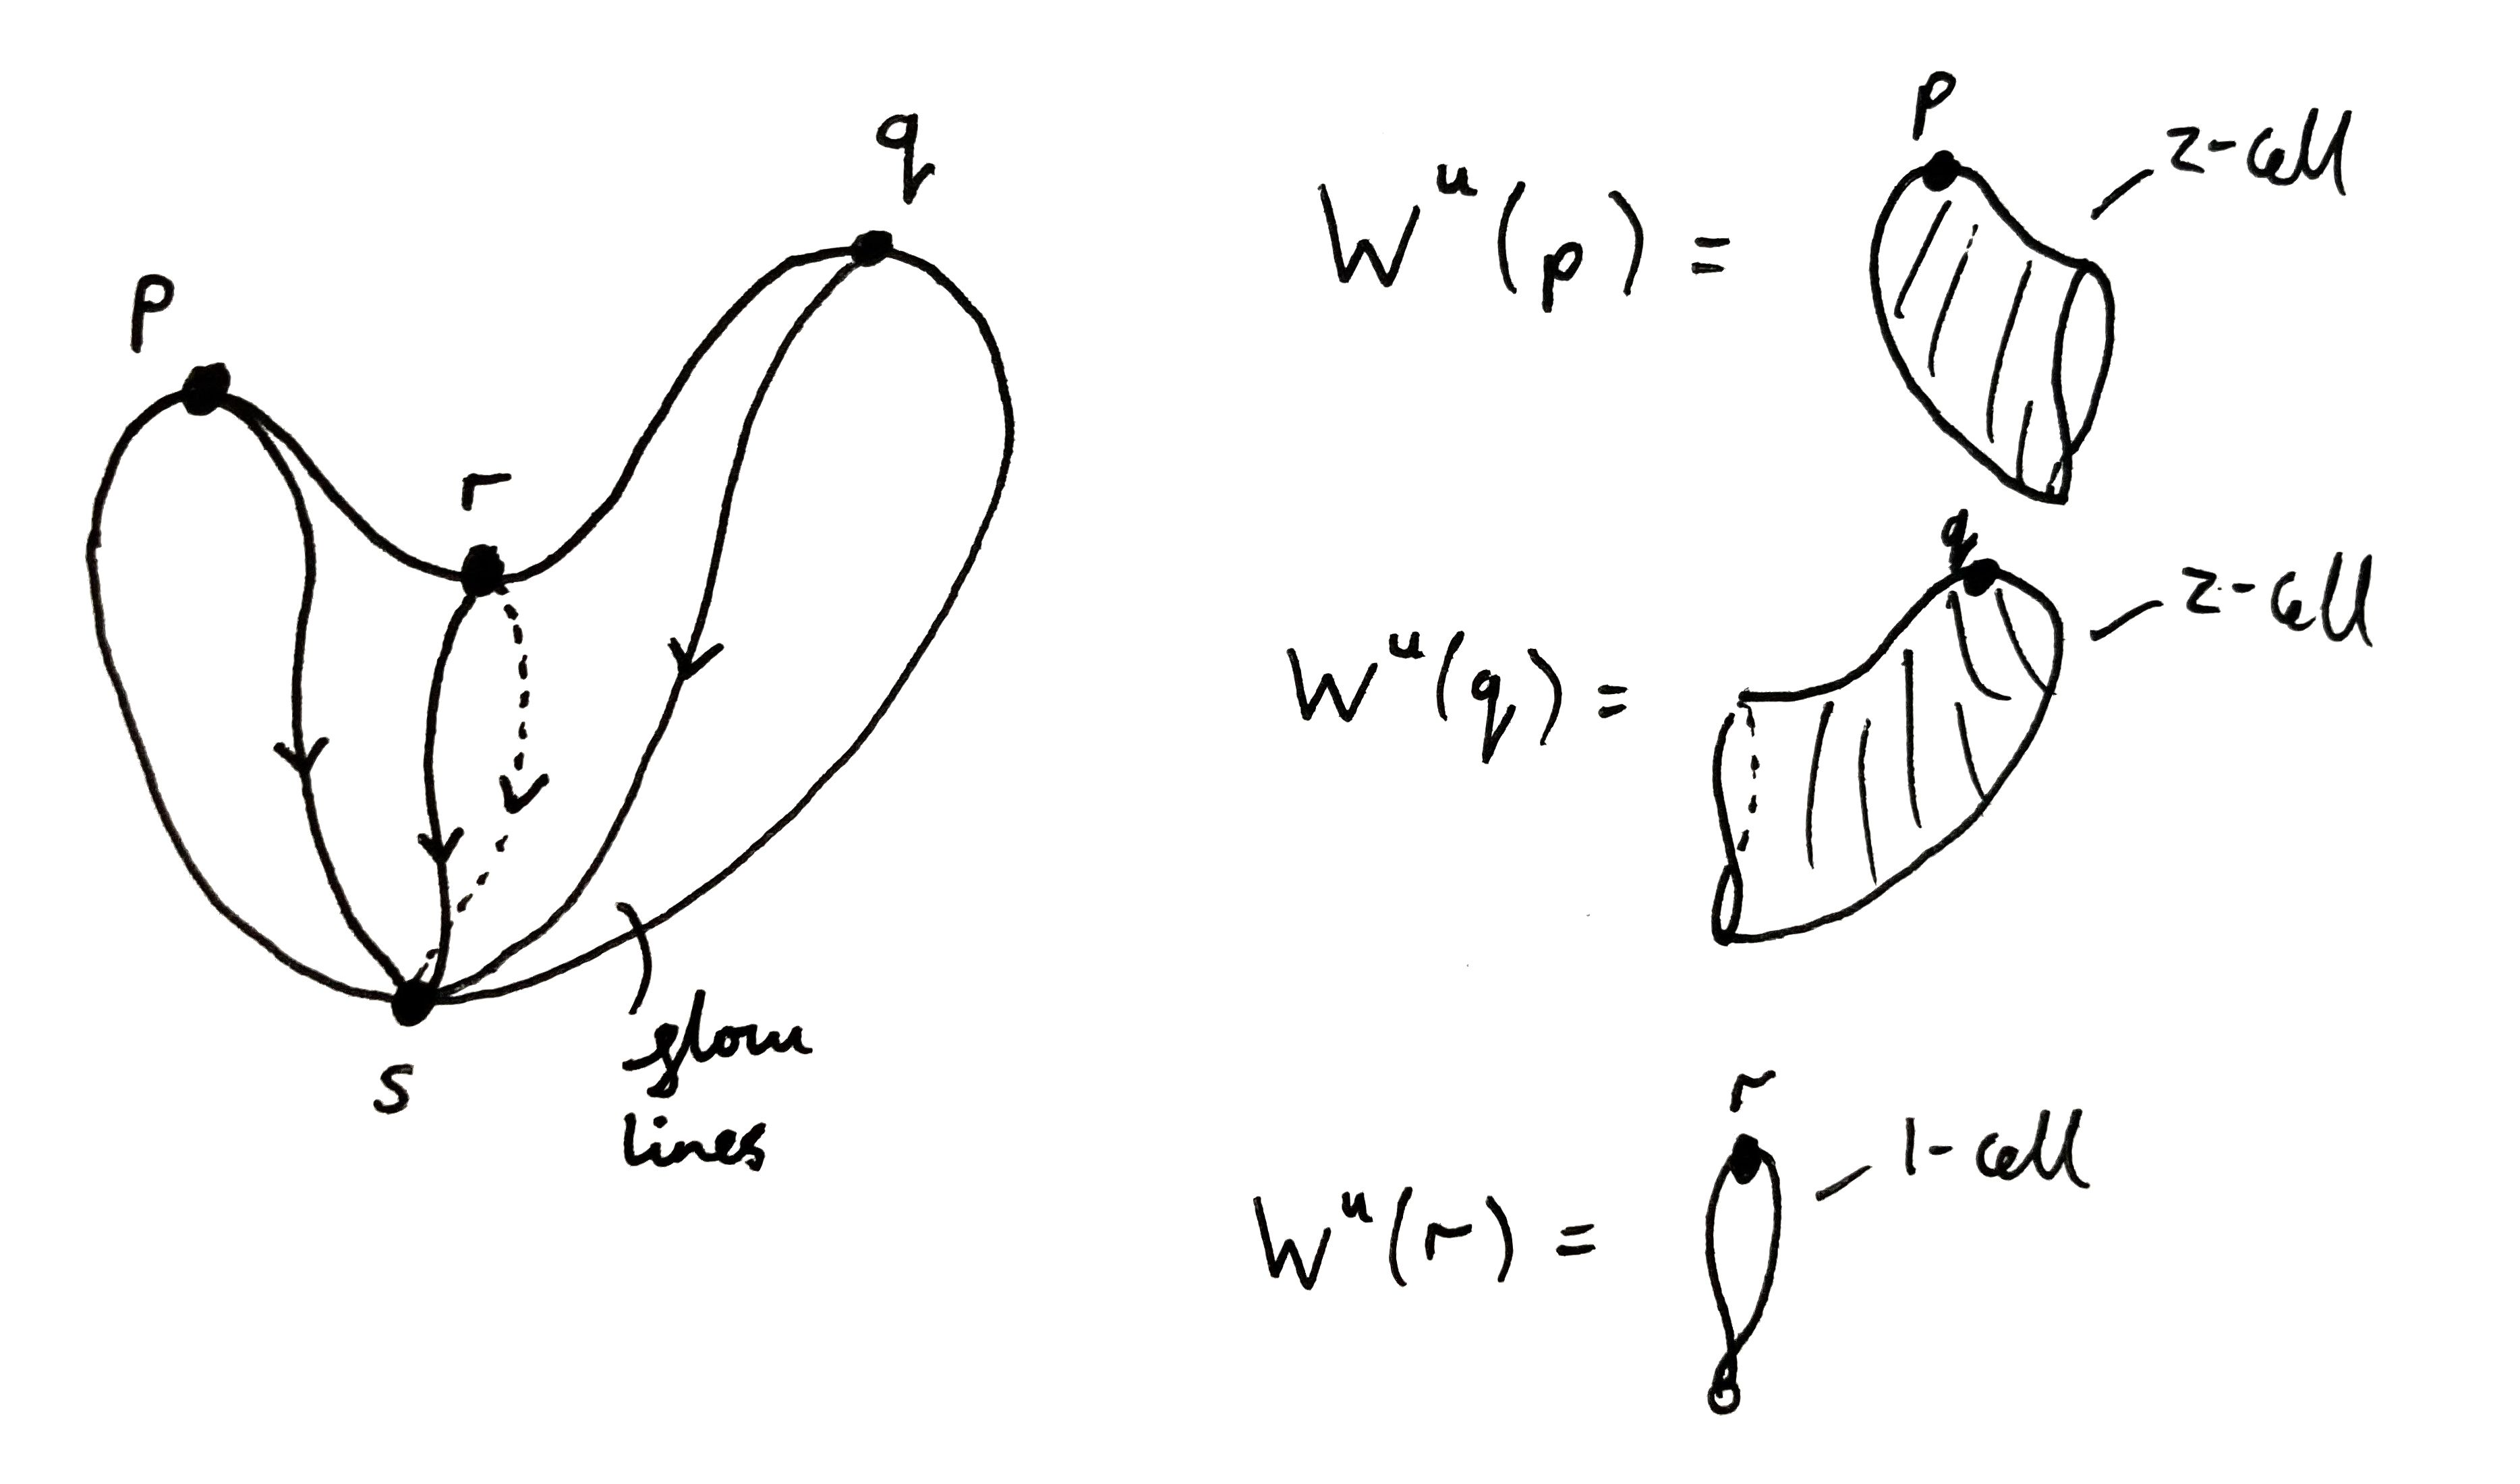
\includegraphics[scale=0.1]{morse_unstable}
\end{center}

\begin{proposition}
    For $p\in\Crit(f)$, $W^u(p)\cong\mathring D^{\ind(p)}$ is an open disc of
    dimension $\ind(p)$.
\end{proposition}

\begin{proof}[Sketch proof]
    The flow eventually brings $W^u(p)$ into a neighbourhood of $p$, and we can
    use the Morse lemma to see that in suitable coordinates it is then the
    interior of the attached $i$-cell seen previously.
\end{proof}

Similarly, the stable manifold $W^s(p)$ is a disc of dimension $n-\ind(p)$.
(There is a duality using the two Morse functions $f$ and $-f$.)

The unstable manifolds hence give a natural cell complex structure. What are the
boundary maps? Consider our example, take a flow line from $p$ to $s$ and
``deform'' it towards the boundary. It can be freely deformed until it
encounters another critical point, at which point it becomes a ``broken
trajectory''.
\begin{center}
    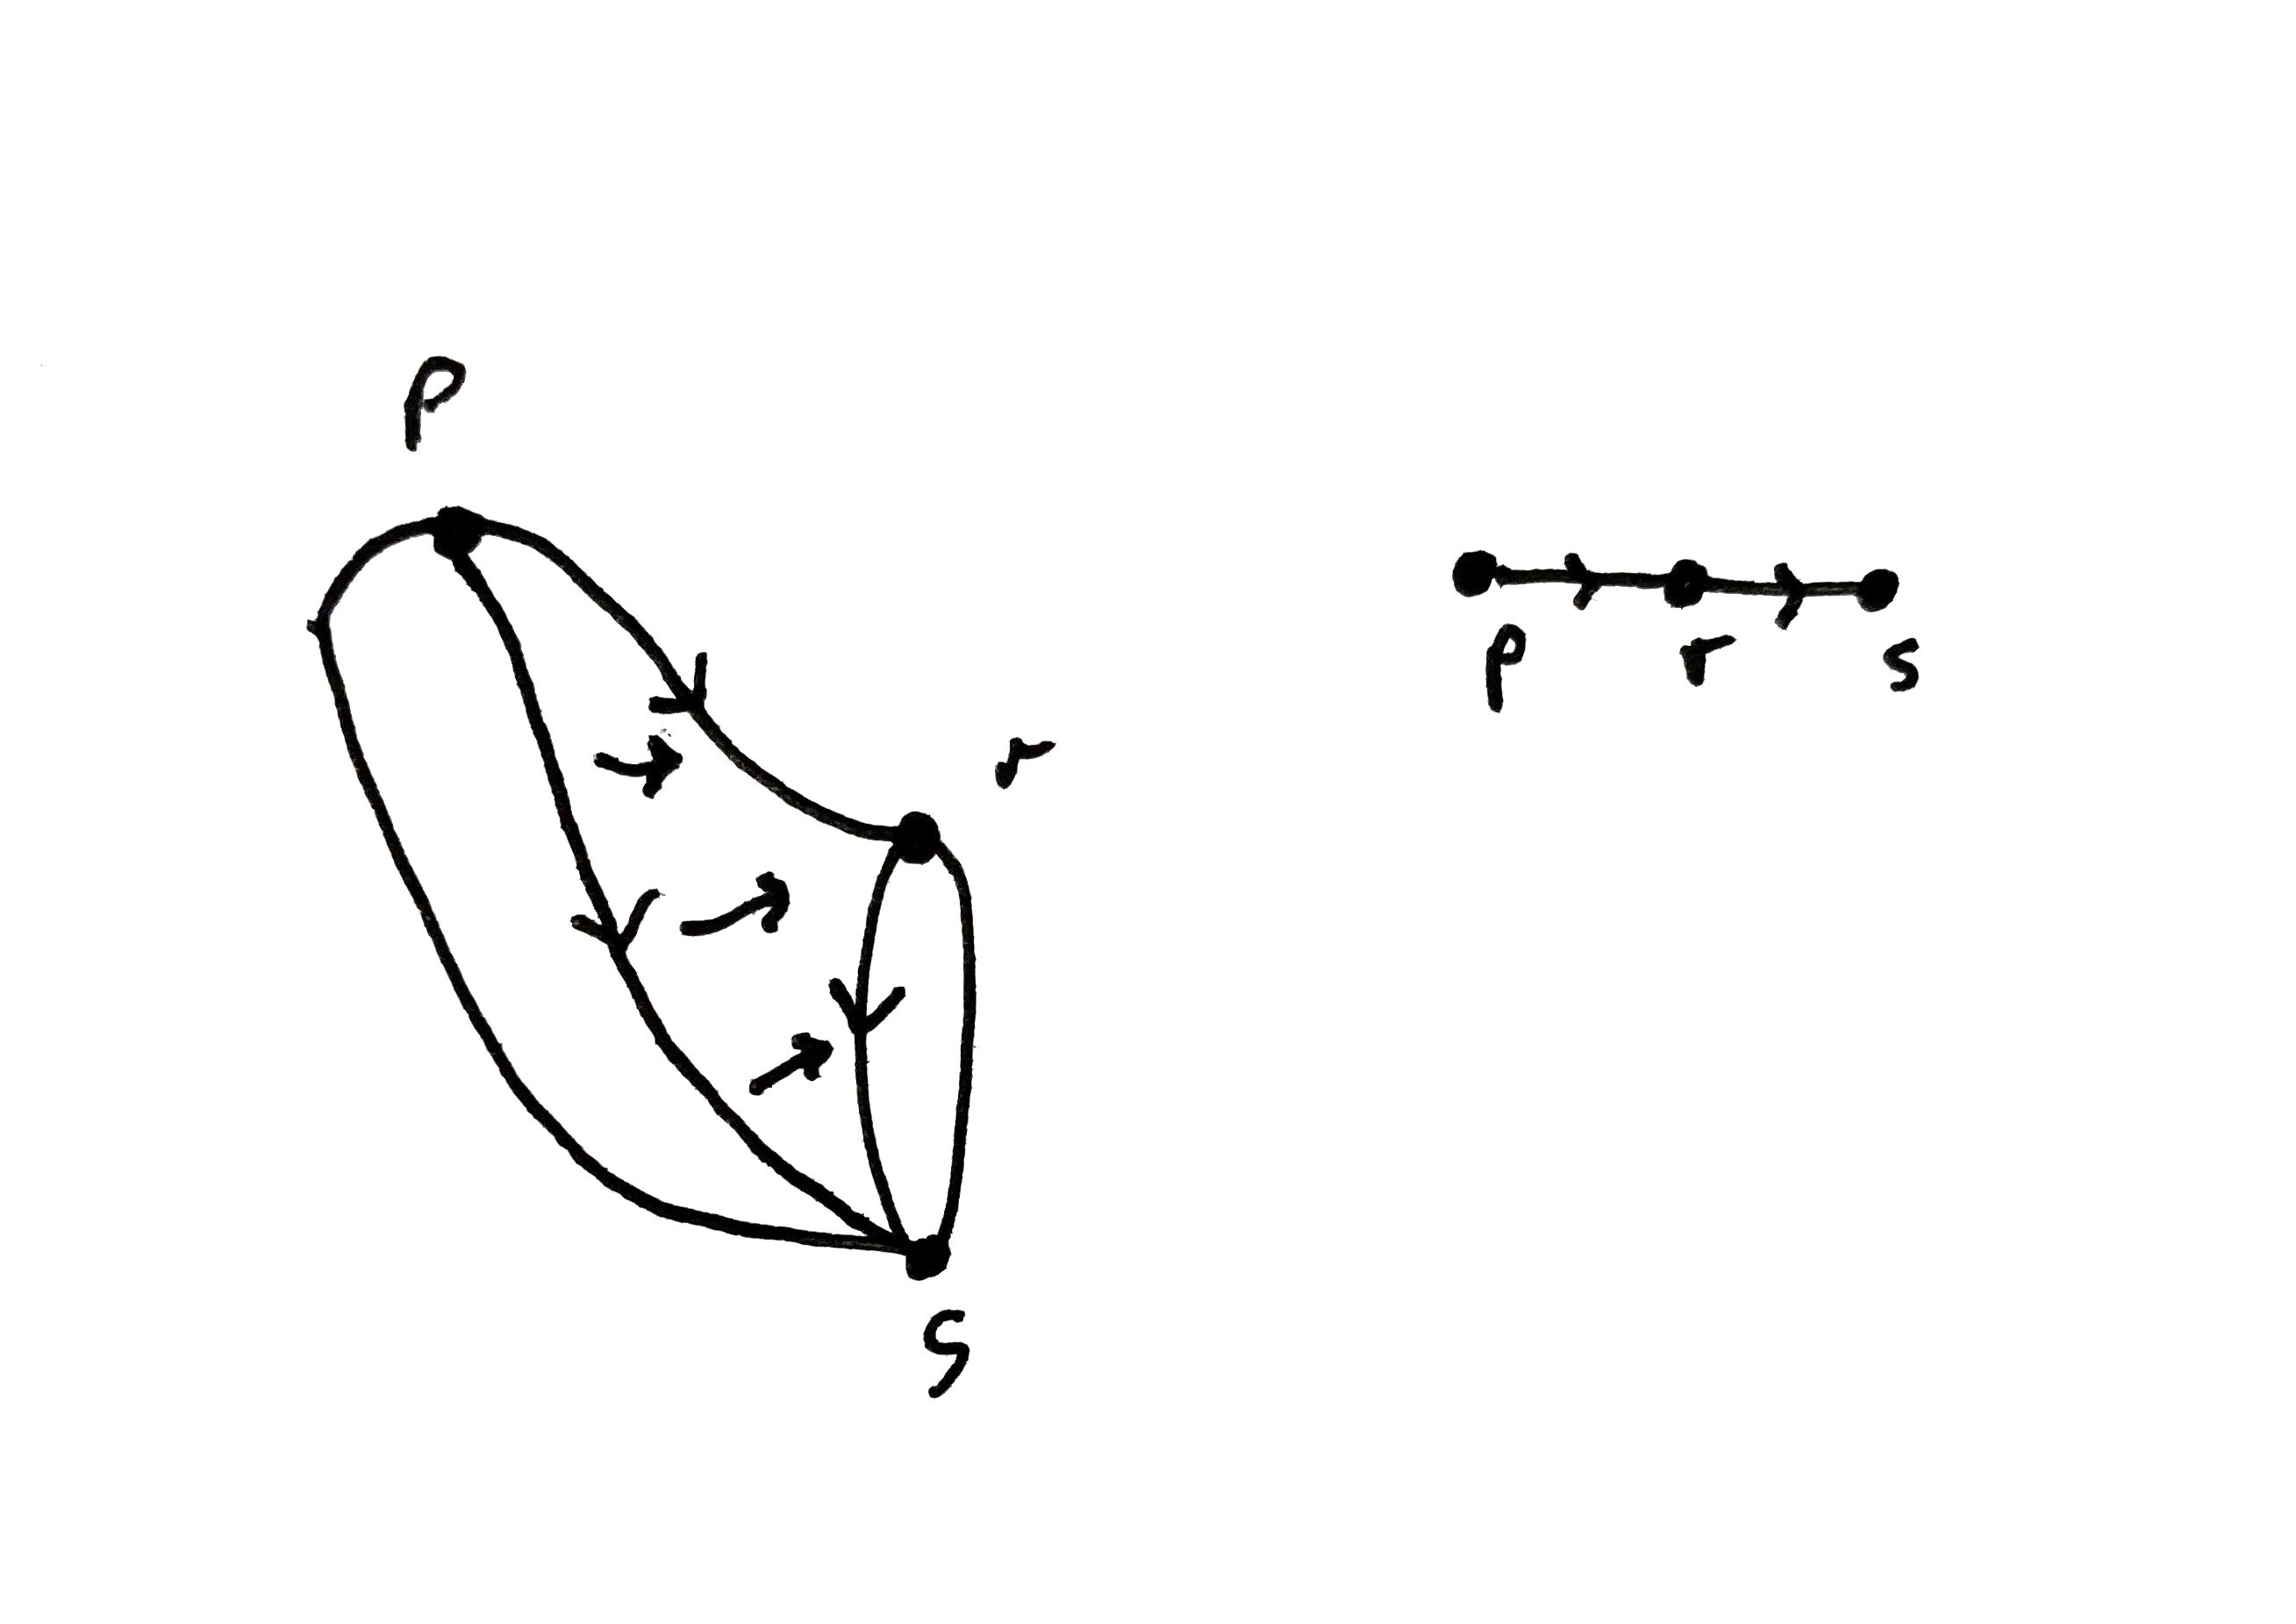
\includegraphics[scale=0.1]{morse_broken}
\end{center}

\begin{theorem}
    $\overbrace{\text{Under some condition on $f$}}
    ^{\text{If $f$ is Morse--Smale}}$, the boundary is given by
    \begin{equation*}
        \partial W^u(p) = \sum_{\ind(q)=\ind(p)-1}n_{pq}\cdot\overline W^u(q),
    \end{equation*}
    where $n_{pq}$ is the number of flow lines from $p$ to $q$, counted with
    appropriate signs.
\end{theorem}

Note that $W^u(p)$ has dimension $\ind(p)$, and $W^s(q)$ has dimension
$n-\ind(p)+1$, so if they are transverse $W^u(p)\cap W^s(q)$ has dimension 1 and
there are only finitely many flow lines from $p$ to $q$.

\begin{definition}
    The function $f$ is called \emph{Morse--Smale} if for all $p,q\in\Crit(f)$
    we have $W^s(p)\pitchfork W^u(q)$, i.e. the stable and unstable manifolds
    intersect transversely.
\end{definition}

With these $n_{pq}$'s we then get a chain complex for a Morse--Smale function
$f$, computing the cellular homology of $M$:
\begin{equation*}
    C_k = \bigoplus_{\ind(p)=k}\Z\cdot p, \qquad
    \partial p=\sum_{\substack{\ind(q)=\ind(p)-1}}n_{pq}\cdot q.
\end{equation*}

\subsection*{Morse inequalities}

\begin{theorem}
    Let $N_k=\rank C_k$. We have
    \begin{equation*}
        \sum_{i=0}^k(-1)^{k-i}N_i\ge\sum_{i=0}^k(-1)^{k-i}b_i(M),
    \end{equation*}
    with equality when $n=k$. Moreover $N_i\ge b_i(M)$.
\end{theorem}

\begin{proof}
    This is a general statement about chain complexes.
\end{proof}

\begin{remark}
    The case $n=k$ computes the Euler characteristic. From $N_i\ge b_i(M)$ we
    can deduce the existence of critical points for Morse functions from the
    topology of $M$.
\end{remark}

We can restrict more than just homology with Morse theory:

\begin{theorem}
    Suppose that $f$ is Morse with no critical points of index 1. Then $M$ is
    simply-connected.
\end{theorem}

\begin{proof}
    Note that $H_1(M)=0$ by the Morse inequalities, but this is not enough. By
    Sard's theorem, we can homotope any loop in $M$ to be transverse to all
    stable manifolds. Then it can only intersect the index 0 ones, so the loop
    is contained in a single cell, a disc of dimension at least 2, and hence
    contracts.
\end{proof}

\subsection*{Exercises}

\begin{exercise}
    Check that the following untilted torus example is not Morse--Smale:
    \begin{center}
        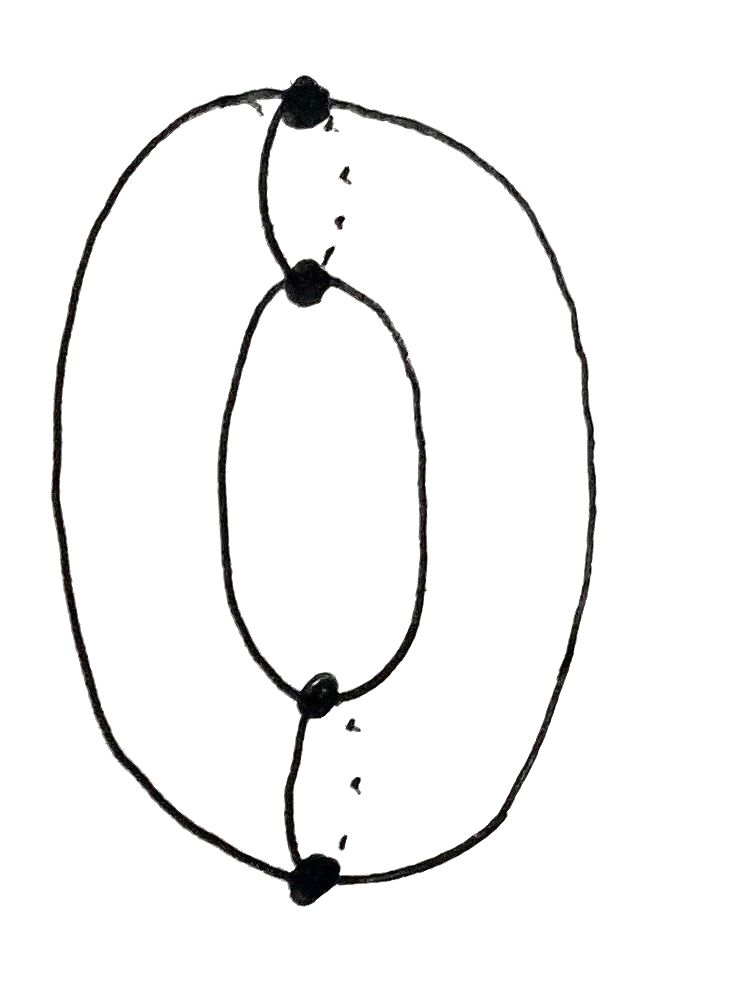
\includegraphics[scale=0.1]{morse_smale}
    \end{center}
    Tilt it slightly to fix this, and compute the Morse complex.
\end{exercise}

\begin{exercise}
    Show that the Betti numbers satisfy Poincar\'e duality
    $b_k(M)=b_{n-k}(M)$ using the Morse complex. (Recall that
    $b_k(M)=\rank H_k(M;\Z)$.)
\end{exercise}

\begin{exercise}
    Suppose $f$ is a Morse function with exactly two critical points. Show
    that $M\approx_\homeo S^n$.
\end{exercise}

\begin{exercise}
    Is it true that for any $M$ there exists a Morse function $f$ with
    $N_k=b_k(M)$?
\end{exercise}

\begin{exercise}
    Suppose $f$ is Morse, and $X=\nabla f$. Show that the index of $X$
    (i.e. the signed count of the zeros of $X$) is the Euler characteristic
    $\chi(M)$. This is the starting point for one of the proofs of the
    Poincar\'e--Hopf theorem.
\end{exercise}

\begin{exercise}
    Take $M=\CP^n$, with
    \begin{equation*}
        f([z_0:\cdots:z_n]) = \frac{\sum_jj|z_j|^2}{\sum_j|z_j|^2}.
    \end{equation*}
    Show that $f$ is Morse, and use it to compute the homology.
\end{exercise}

\subsection*{Notable applications}

\begin{enumerate}[label=\textbf{\Roman* -}]
    \item Generalized Poincar\'e conjecture: If $M$ is a manifold of dimension
        $n$ homotopy equivalent to $S^n$, then $M$ is homeomorphic to $S^n$.

        In dimensions $n\ge5$ this can be proved using Morse theory. (See
        Milnor's ``Lectures on the $h$-cobordism theorem''.)

    \item ``Morse theory'' on infinite-dimensional spaces:
        \begin{enumerate}[label=(\alph*)]
            \item Low-dimensional topology; instanton homology
                (gauge theoretical functionals).

            \item Symplectic geometry (counting closed orbits, Floer homology).

            \item Riemannian geometry:
                \begin{itemize}
                    \item Length functional on path space; critical points are
                        geodesics, index related to Jacobi fields.

                    \item Bott periodicity:
                        $\pi_i(U(\infty))=\pi_{i+2}(U(\infty))$.

                    \item Finding closed geodesics:
                        \begin{theorem}[Birkhoff]
                            For all metrics $g$ on $S^2$ there exists a
                            non-trivial closed geodesic.
                        \end{theorem}

                        \begin{proof}[``Proof'']
                            Assume Morse theory works on the loop space
                            $\Omega(S^2)$ for the length functional. Since
                            $\pi_i(\Omega(S^2))=\pi_{i+1}(S^2)$ we have
                            $\pi_1(\Omega(S^2))=\pi_2(S^2)=\Z$, so there must be
                            a critical point of index 1 by the Morse
                            inequalities.
                        \end{proof}

                    \item More generally, interactions between curvature and
                        topology:
                        \begin{itemize}
                            \item Sphere theorem: $\frac{1}{4}<K\le 1$ implies
                                $M\approx_\homeo S^n$.

                            \item Minimal surface theory (critical points of
                                area functional).
                        \end{itemize}
                \end{itemize}
        \end{enumerate}
\end{enumerate}

\subsection*{Bonus exercises}

\begin{enumerate}[label=(\arabic*)]
    \item View the torus as the square $[0,2\pi]\times[0,2\pi]$ with side
        identifications, and consider the function
        $(x,y)\mapsto\sin(x)+\sin(y)$. Compute the Morse complex.

    \item If $A$ be a self-adjoint operator on $\R^n$, then
        \begin{equation*}
            x \mapsto \frac{\langle Ax,x\rangle}{\langle x,x\rangle}
        \end{equation*}
        is invariant under $x\mapsto\lambda x$, and hence induces a function
        $f_A:\RP^n\to\R$. When is it Morse? Describe critical points and their
        indices when it is.
\end{enumerate}

\end{document}
